\documentclass[12pt,]{krantz}
\usepackage{lmodern}
\usepackage{amssymb,amsmath}
\usepackage{ifxetex,ifluatex}
\usepackage{fixltx2e} % provides \textsubscript
\ifnum 0\ifxetex 1\fi\ifluatex 1\fi=0 % if pdftex
  \usepackage[T1]{fontenc}
  \usepackage[utf8]{inputenc}
\else % if luatex or xelatex
  \ifxetex
    \usepackage{mathspec}
  \else
    \usepackage{fontspec}
  \fi
  \defaultfontfeatures{Ligatures=TeX,Scale=MatchLowercase}
    \setmonofont[Mapping=tex-ansi,Scale=0.7]{Source Code Pro}
\fi
% use upquote if available, for straight quotes in verbatim environments
\IfFileExists{upquote.sty}{\usepackage{upquote}}{}
% use microtype if available
\IfFileExists{microtype.sty}{%
\usepackage{microtype}
\UseMicrotypeSet[protrusion]{basicmath} % disable protrusion for tt fonts
}{}
\usepackage{hyperref}
\PassOptionsToPackage{usenames,dvipsnames}{color} % color is loaded by hyperref
\hypersetup{unicode=true,
            pdftitle={Panduan Lengkap Analisis Statistika Menggunakan R Commander},
            pdfauthor={Mohammad Rosidi},
            colorlinks=true,
            linkcolor=Maroon,
            citecolor=Blue,
            urlcolor=Blue,
            breaklinks=true}
\urlstyle{same}  % don't use monospace font for urls
\usepackage{natbib}
\bibliographystyle{apalike}
\usepackage{color}
\usepackage{fancyvrb}
\newcommand{\VerbBar}{|}
\newcommand{\VERB}{\Verb[commandchars=\\\{\}]}
\DefineVerbatimEnvironment{Highlighting}{Verbatim}{commandchars=\\\{\}}
% Add ',fontsize=\small' for more characters per line
\usepackage{framed}
\definecolor{shadecolor}{RGB}{248,248,248}
\newenvironment{Shaded}{\begin{snugshade}}{\end{snugshade}}
\newcommand{\AlertTok}[1]{\textcolor[rgb]{0.94,0.16,0.16}{#1}}
\newcommand{\AnnotationTok}[1]{\textcolor[rgb]{0.56,0.35,0.01}{\textbf{\textit{#1}}}}
\newcommand{\AttributeTok}[1]{\textcolor[rgb]{0.77,0.63,0.00}{#1}}
\newcommand{\BaseNTok}[1]{\textcolor[rgb]{0.00,0.00,0.81}{#1}}
\newcommand{\BuiltInTok}[1]{#1}
\newcommand{\CharTok}[1]{\textcolor[rgb]{0.31,0.60,0.02}{#1}}
\newcommand{\CommentTok}[1]{\textcolor[rgb]{0.56,0.35,0.01}{\textit{#1}}}
\newcommand{\CommentVarTok}[1]{\textcolor[rgb]{0.56,0.35,0.01}{\textbf{\textit{#1}}}}
\newcommand{\ConstantTok}[1]{\textcolor[rgb]{0.00,0.00,0.00}{#1}}
\newcommand{\ControlFlowTok}[1]{\textcolor[rgb]{0.13,0.29,0.53}{\textbf{#1}}}
\newcommand{\DataTypeTok}[1]{\textcolor[rgb]{0.13,0.29,0.53}{#1}}
\newcommand{\DecValTok}[1]{\textcolor[rgb]{0.00,0.00,0.81}{#1}}
\newcommand{\DocumentationTok}[1]{\textcolor[rgb]{0.56,0.35,0.01}{\textbf{\textit{#1}}}}
\newcommand{\ErrorTok}[1]{\textcolor[rgb]{0.64,0.00,0.00}{\textbf{#1}}}
\newcommand{\ExtensionTok}[1]{#1}
\newcommand{\FloatTok}[1]{\textcolor[rgb]{0.00,0.00,0.81}{#1}}
\newcommand{\FunctionTok}[1]{\textcolor[rgb]{0.00,0.00,0.00}{#1}}
\newcommand{\ImportTok}[1]{#1}
\newcommand{\InformationTok}[1]{\textcolor[rgb]{0.56,0.35,0.01}{\textbf{\textit{#1}}}}
\newcommand{\KeywordTok}[1]{\textcolor[rgb]{0.13,0.29,0.53}{\textbf{#1}}}
\newcommand{\NormalTok}[1]{#1}
\newcommand{\OperatorTok}[1]{\textcolor[rgb]{0.81,0.36,0.00}{\textbf{#1}}}
\newcommand{\OtherTok}[1]{\textcolor[rgb]{0.56,0.35,0.01}{#1}}
\newcommand{\PreprocessorTok}[1]{\textcolor[rgb]{0.56,0.35,0.01}{\textit{#1}}}
\newcommand{\RegionMarkerTok}[1]{#1}
\newcommand{\SpecialCharTok}[1]{\textcolor[rgb]{0.00,0.00,0.00}{#1}}
\newcommand{\SpecialStringTok}[1]{\textcolor[rgb]{0.31,0.60,0.02}{#1}}
\newcommand{\StringTok}[1]{\textcolor[rgb]{0.31,0.60,0.02}{#1}}
\newcommand{\VariableTok}[1]{\textcolor[rgb]{0.00,0.00,0.00}{#1}}
\newcommand{\VerbatimStringTok}[1]{\textcolor[rgb]{0.31,0.60,0.02}{#1}}
\newcommand{\WarningTok}[1]{\textcolor[rgb]{0.56,0.35,0.01}{\textbf{\textit{#1}}}}
\usepackage{longtable,booktabs}
\usepackage{graphicx,grffile}
\makeatletter
\def\maxwidth{\ifdim\Gin@nat@width>\linewidth\linewidth\else\Gin@nat@width\fi}
\def\maxheight{\ifdim\Gin@nat@height>\textheight\textheight\else\Gin@nat@height\fi}
\makeatother
% Scale images if necessary, so that they will not overflow the page
% margins by default, and it is still possible to overwrite the defaults
% using explicit options in \includegraphics[width, height, ...]{}
\setkeys{Gin}{width=\maxwidth,height=\maxheight,keepaspectratio}
\IfFileExists{parskip.sty}{%
\usepackage{parskip}
}{% else
\setlength{\parindent}{0pt}
\setlength{\parskip}{6pt plus 2pt minus 1pt}
}
\setlength{\emergencystretch}{3em}  % prevent overfull lines
\providecommand{\tightlist}{%
  \setlength{\itemsep}{0pt}\setlength{\parskip}{0pt}}
\setcounter{secnumdepth}{5}
% Redefines (sub)paragraphs to behave more like sections
\ifx\paragraph\undefined\else
\let\oldparagraph\paragraph
\renewcommand{\paragraph}[1]{\oldparagraph{#1}\mbox{}}
\fi
\ifx\subparagraph\undefined\else
\let\oldsubparagraph\subparagraph
\renewcommand{\subparagraph}[1]{\oldsubparagraph{#1}\mbox{}}
\fi

%%% Use protect on footnotes to avoid problems with footnotes in titles
\let\rmarkdownfootnote\footnote%
\def\footnote{\protect\rmarkdownfootnote}

%%% Change title format to be more compact
\usepackage{titling}

% Create subtitle command for use in maketitle
\providecommand{\subtitle}[1]{
  \posttitle{
    \begin{center}\large#1\end{center}
    }
}

\setlength{\droptitle}{-2em}

  \title{Panduan Lengkap Analisis Statistika Menggunakan R Commander}
    \pretitle{\vspace{\droptitle}\centering\huge}
  \posttitle{\par}
    \author{Mohammad Rosidi}
    \preauthor{\centering\large\emph}
  \postauthor{\par}
      \predate{\centering\large\emph}
  \postdate{\par}
    \date{2020-01-07}

\usepackage{booktabs}
\usepackage{longtable}
\usepackage[bf,singlelinecheck=off]{caption}

\usepackage{framed,color}
\definecolor{shadecolor}{RGB}{248,248,248}

\renewcommand{\textfraction}{0.05}
\renewcommand{\topfraction}{0.8}
\renewcommand{\bottomfraction}{0.8}
\renewcommand{\floatpagefraction}{0.75}

\renewenvironment{quote}{\begin{VF}}{\end{VF}}
\let\oldhref\href
\renewcommand{\href}[2]{#2\footnote{\url{#1}}}

\ifxetex
  \usepackage{letltxmacro}
  \setlength{\XeTeXLinkMargin}{1pt}
  \LetLtxMacro\SavedIncludeGraphics\includegraphics
  \def\includegraphics#1#{% #1 catches optional stuff (star/opt. arg.)
    \IncludeGraphicsAux{#1}%
  }%
  \newcommand*{\IncludeGraphicsAux}[2]{%
    \XeTeXLinkBox{%
      \SavedIncludeGraphics#1{#2}%
    }%
  }%
\fi

\makeatletter
\newenvironment{kframe}{%
\medskip{}
\setlength{\fboxsep}{.8em}
 \def\at@end@of@kframe{}%
 \ifinner\ifhmode%
  \def\at@end@of@kframe{\end{minipage}}%
  \begin{minipage}{\columnwidth}%
 \fi\fi%
 \def\FrameCommand##1{\hskip\@totalleftmargin \hskip-\fboxsep
 \colorbox{shadecolor}{##1}\hskip-\fboxsep
     % There is no \\@totalrightmargin, so:
     \hskip-\linewidth \hskip-\@totalleftmargin \hskip\columnwidth}%
 \MakeFramed {\advance\hsize-\width
   \@totalleftmargin\z@ \linewidth\hsize
   \@setminipage}}%
 {\par\unskip\endMakeFramed%
 \at@end@of@kframe}
\makeatother

\usepackage{makeidx}
\makeindex

\urlstyle{tt}

\usepackage{amsthm}
\makeatletter
\def\thm@space@setup{%
  \thm@preskip=8pt plus 2pt minus 4pt
  \thm@postskip=\thm@preskip
}
\makeatother

\frontmatter

\begin{document}
\maketitle

%\cleardoublepage\newpage\thispagestyle{empty}\null
%\cleardoublepage\newpage\thispagestyle{empty}\null
%\cleardoublepage\newpage
\thispagestyle{empty}
\begin{center}

\includegraphics{images/dedication.pdf}
\end{center}

\setlength{\abovedisplayskip}{-5pt}
\setlength{\abovedisplayshortskip}{-5pt}

{
\hypersetup{linkcolor=black}
\setcounter{tocdepth}{2}
\tableofcontents
}
\listoftables
\listoffigures
\hypertarget{pengantar}{%
\chapter*{Pengantar}\label{pengantar}}


\mainmatter

\hypertarget{intro}{%
\chapter{\texorpdfstring{Pengenalan \texttt{R} dan \texttt{R\ Commander}}{Pengenalan R dan R Commander}}\label{intro}}

Pada Chapter \ref{intro} pembaca akan belajar mengenai perangkat lunak \texttt{R}, \texttt{Rcmdr}, dan cara instalasi keduanya. Pembaca juga akan belajar tampilan antar muka dan fitur apa saja yang disediakan pada \texttt{Rcmdr}. Detail terkait fitur-fitur \texttt{Rcmdr} yang digunakan dalam melakukan analisis statistika akan dijelaskan pada Chapter-Chapter selanjutnya.

\hypertarget{whatR}{%
\section{\texorpdfstring{Apa Itu \texttt{R} dan \texttt{Rcmdr}?}{Apa Itu R dan Rcmdr?}}\label{whatR}}

\texttt{R} Merupakan bahasa yang digunakan dalam komputasi \textbf{statistik} yang pertama kali dikembangkan oleh \textbf{Ross Ihaka} dan \textbf{Robert Gentlement} di University of Auckland New Zealand yang merupakan akronim dari nama depan kedua pembuatnya. Sebelum \texttt{R} dikenal ada \texttt{S} yang dikembangkan oleh \textbf{John Chambers} dan rekan-rekan dari \textbf{Bell Laboratories} yang memiliki fungsi yang sama untuk komputasi statistik. Hal yang membedakan antara keduanya adalah \texttt{R} merupakan sistem komputasi yang bersifat gratis.Logo \texttt{R} dapat dilihat pada Gambar \ref{fig:Logo}.

\begin{figure}

{\centering 
\includegraphics[width=0.4\linewidth]{./images/chp1/r-icon} 

}

\caption{Logo R.}\label{fig:Logo}
\end{figure}

\texttt{Rcmdr} atau \texttt{R\ Commander} (Fox, 2005) merupakan paket yang menyediakan tampilan antar muka (GUI) yang memungkinkan pengguna untuk berinteraksi dengan \texttt{R} melalui \emph{point-and-click}. Keuntungan cara berinteraksi semacam itu membuat pengguna dapat lebih memfokuskan diri pada metode statistik yang digunakannya dibandingkan melakukan penulisan sintaks program untuk memperoleh hasil perhitungan statistik yang sama. Selain itu, sintaks yang digunakan program untuk melakukan perhitungan ditampilkan ke dalam editor yang tersedia pada jendela \texttt{Rcmdr} secara otomatis. Hal tersebut dapat mempermudah analis dalam mempelajari kode apa saja yang perlu diketikkan untuk menghasilkan hasil perhitungan statistik yang analis perlukan.

\hypertarget{install}{%
\section{\texorpdfstring{Memasang \texttt{R} dan \texttt{R\ Commander}}{Memasang R dan R Commander}}\label{install}}

Pada Chapter \ref{install} pembaca akan belajar bagaimana cara memasang \texttt{R} dan \texttt{R\ Commander} Pembaca juga akan belajar bagaimana cara menjalankan \texttt{R\ Commander} dari \texttt{R}.

Untuk memperoleh \texttt{R} pembaca dapat melakukan unduh pada situs \href{https://cran.r-project.org/}{CRAN}. Tampilan situs untuk mengunduh \texttt{R} ditampilkan pada Gambar \ref{fig:unduh}.

\begin{figure}

{\centering 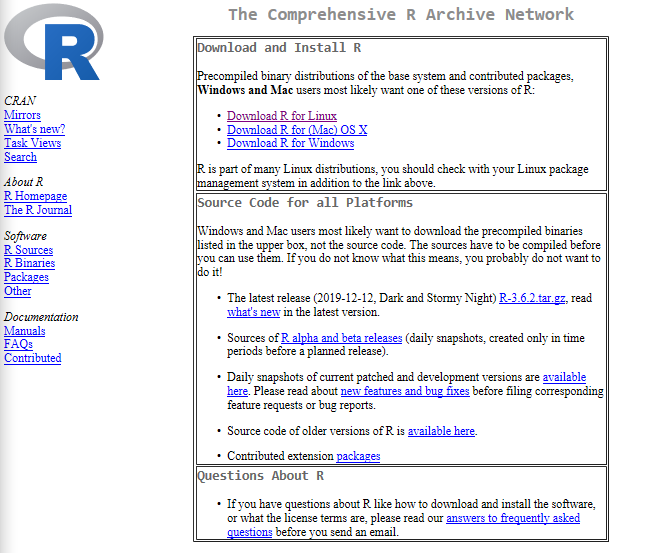
\includegraphics[width=0.8\linewidth]{./images/chp1/CRAN} 

}

\caption{Tampilan situs CRAN.}\label{fig:unduh}
\end{figure}

\hypertarget{memasang-r-pada-windows}{%
\subsection{\texorpdfstring{Memasang \texttt{R} pada Windows}{Memasang R pada Windows}}\label{memasang-r-pada-windows}}

\texttt{R\ for\ Windows} dapat diperoleh melalui tautan \href{https://cran.r-project.org/}{CRAN}. Berdasarkan halaman situs diketahui bahwa saat ini versi \texttt{R} yang tersedia adalah versi \texttt{R\ 3.6.2}. Tampilan situs tersebut dapat dilihat pada Gambar \ref{fig:rwin}.

\begin{figure}

{\centering 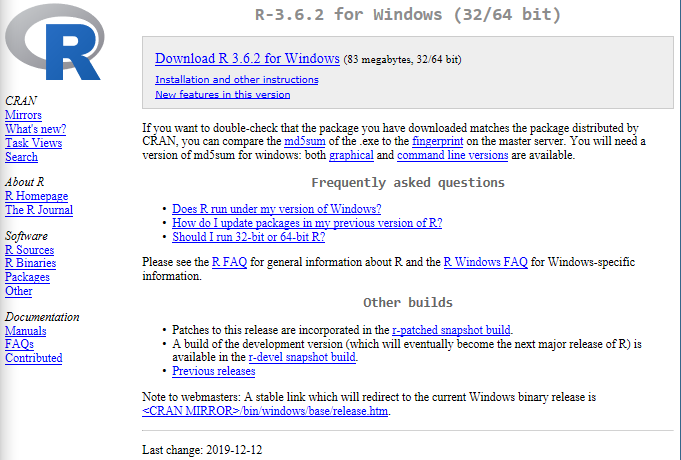
\includegraphics[width=0.8\linewidth]{./images/chp1/rwin} 

}

\caption{Tampilan halaman situs R untuk mengunduh R for windows.}\label{fig:rwin}
\end{figure}

Tahapan instalasi:

\begin{enumerate}
\def\labelenumi{\arabic{enumi}.}
\tightlist
\item
  \emph{Double click} \texttt{R\ installer} yang telah di unduh sehingga muncul jendela instalasi.
\item
  Pilih bahasa yang akan digunakan.
\item
  Pembaca hanya perlu menekan tombol \emph{next} pada jedela yang muncul untuk memasang \texttt{R} dengan konfigurasi \emph{default}.
\item
  Setelah proses instalasi selesai pembaca dapat menekan tombol \emph{finish}.
\end{enumerate}

\begin{figure}

{\centering 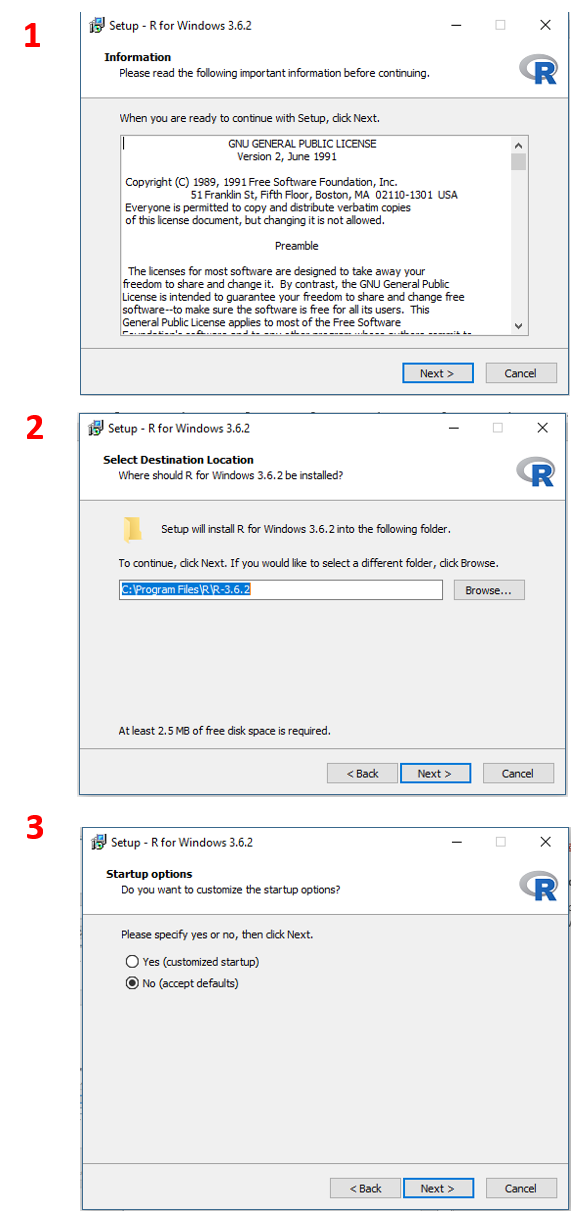
\includegraphics[width=0.7\linewidth]{./images/chp1/installrwin} 

}

\caption{Tampilan tahapan kunci proses instalasi R for Windows.}\label{fig:installrwin}
\end{figure}

Untuk lebih lengkapnya, pembaca dapat menyaksikan video yang dibuat oleh \href{https://www.youtube.com/watch?v=9-RrkJQQYqY}{Xperimental Learning}.

\hypertarget{memasang-r-pada-mac-os-x}{%
\subsection{\texorpdfstring{Memasang \texttt{R} pada Mac OS X}{Memasang R pada Mac OS X}}\label{memasang-r-pada-mac-os-x}}

Sebelum melakukan proses instalasi pastikan Mac OS X yang pembaca miliki \emph{up to date}. Untuk mengetahuinya pembaca dapat menjalakan \emph{Software Update} dari menu yang berada pada pojok kiri atas layar. Hal tersebut penting sebab \texttt{R} mengasumsikan bahwa sistem yang kita miliki telah \emph{up to date}.

\texttt{R\ for\ Mac\ OS\ X} dapat diperoleh melalui tautan \href{https://www.xquartz.org/}{XQuartz}. Selanjutnya pembaca tinggal mengunduh file yang memiliki format file \texttt{XQuartz-x.y.zz.dmg}. Tampilan situs tersebut dapat dilihat pada Gambar \ref{fig:rmac}.

\begin{figure}

{\centering 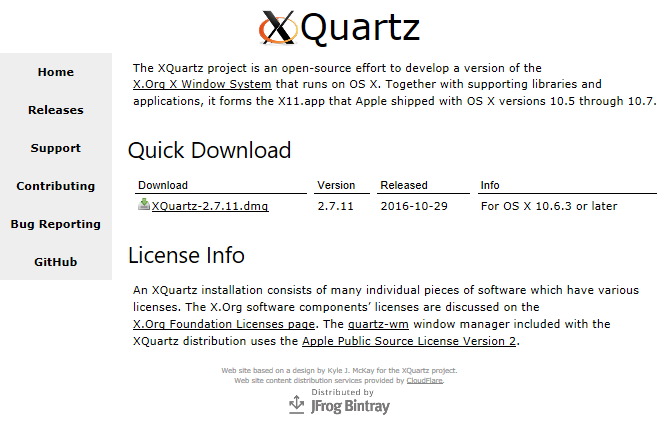
\includegraphics[width=0.8\linewidth]{./images/chp1/rmac} 

}

\caption{Tampilan halaman situs XQuartz.}\label{fig:rmac}
\end{figure}

Tahapan instalasi:

\begin{enumerate}
\def\labelenumi{\arabic{enumi}.}
\tightlist
\item
  Mengunduh \emph{disk image file} \texttt{XQuatz-x.y.zz.dmg} dimana \texttt{x.y.zz} merupakan versi dari \texttt{XQuartz}.
\item
  \emph{Double click} pada file tersebut. Jika pembaca menemukan file \texttt{XQuatz.pkg}, \emph{Double click} pada file tersebut. Lakukan klik pada tombol \emph{continue} untuk konfigurasi instalasi \emph{default}.
\item
  Setelah proses instalasi \emph{log out} dari sesi komputer pembaca sekarang atau lakukan \emph{reboot/restart} dan masuk kembali menggunakan akun Mac OS X pembaca.
\end{enumerate}

\begin{figure}

{\centering 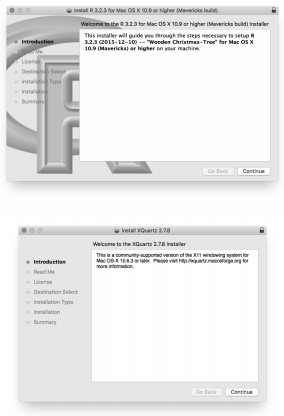
\includegraphics[width=0.7\linewidth]{./images/chp1/installrmac} 

}

\caption{Tampilan awal proses instalasi R for Mac OS X (Sumber: Fox, 2017).}\label{fig:installrmac}
\end{figure}

Alternatif metode instalasi lainnya dapat pembaca baca pada artikel yang ditulis oleh \href{https://medium.com/@GalarnykMichael/install-r-and-rstudio-on-mac-e911606ce4f4}{Galarnyk(2017)}.

\hypertarget{memasang-r-pada-linux-dan-unix}{%
\subsection{\texorpdfstring{Memasang \texttt{R} pada Linux dan Unix}{Memasang R pada Linux dan Unix}}\label{memasang-r-pada-linux-dan-unix}}

Berdasarkan situs CRAN, \texttt{R} tersedia pada sejumlah distribusi linux, seperti: Debian, RedHat, SUSE, dan Ubuntu. Jika pembaca memiliki sistem linux atau unix yang tidak \emph{compatible} berdasarkan daftar distribusi linux yang tersedia, pembaca perlu melakukan kompilasi \texttt{R} dari kode sumber. Prosedur untuk melakukan hal tersebut dijelaskan pada halaman \href{https://cran.r-project.org/doc/FAQ/RFAQ.html}{R FAQ}.

\hypertarget{installrcmdr}{%
\subsection{\texorpdfstring{Memasang \texttt{R\ Commander}}{Memasang R Commander}}\label{installrcmdr}}

Terdapat dua buah cara untuk memasang \texttt{R\ Commander} pada \texttt{R}, yaitu: melalui sintaks pada \texttt{R} \emph{Console} dan melalui menu \texttt{Packages}. Untuk melakukan instalasi menggunakan \texttt{R} \emph{Console}, jalankan sintaks berikut:

\begin{Shaded}
\begin{Highlighting}[]
\KeywordTok{install.packages}\NormalTok{(}\StringTok{"Rcmdr"}\NormalTok{)}
\end{Highlighting}
\end{Shaded}

Program selanjutnya akan memasang \texttt{R\ Commander} dan paket-paket lain yang menjadi \emph{dependency}-nya.

Untuk instalasi melalui menu \texttt{Packages}, langkah-langkah yang perlu dilakukan adalah sebagai berikut:

\begin{enumerate}
\def\labelenumi{\arabic{enumi}.}
\tightlist
\item
  Jalankan \texttt{R} dengan cara \emph{double click} pada \emph{shortcut} \texttt{R} yang ada pada desktop atau melalui menu sistem operasi yang pembaca miliki.
\item
  Klik pada \texttt{Packages/Install\ package(s)...}.
\item
  Pilih CRAN \emph{mirror} yang tersedia, klik OK. Pembaca dapat pula memilih CRAN \emph{mirror} dari Indonesia. Jika gagal pembaca dapat mencobanya dengan menggunakan CRAN \emph{mirror} dari negara lain.
\item
  Pilih paket \texttt{Rcmdr}, klik OK.
\item
  Saat pertama kali proses instalasi akan muncul dialog yang berisi apakah pembaca setuju jika \texttt{R} membuat sebuah \emph{directory} yang berisi paket \texttt{Rcmdr}.
\item
  \texttt{R} akan mengunduh paket \texttt{Rcmdr} dan \emph{dependency}-nya.
\end{enumerate}

\begin{figure}

{\centering 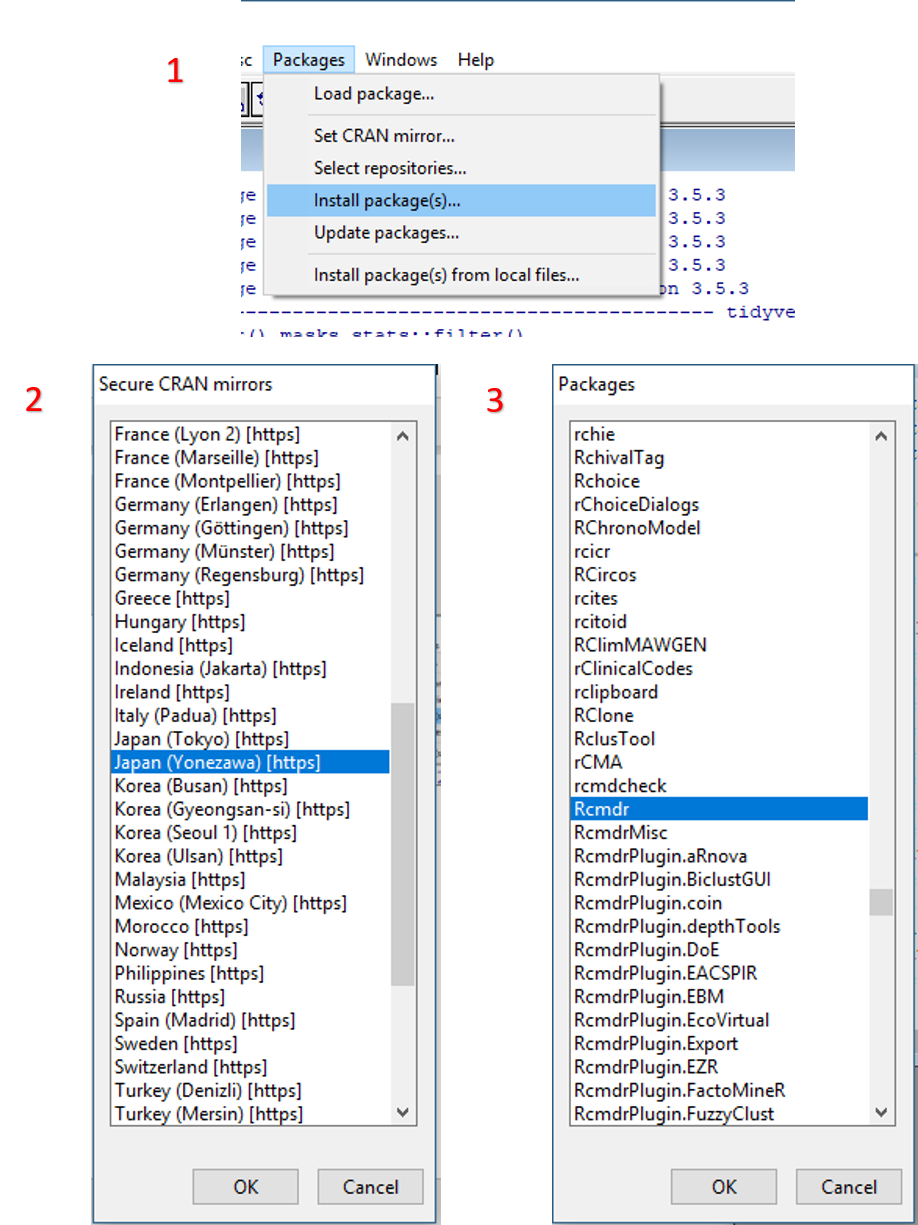
\includegraphics[width=0.7\linewidth]{./images/chp1/installrcmdr} 

}

\caption{Tampilan proses instalasi menggunakan menu Packages.}\label{fig:installrcmdr}
\end{figure}

\hypertarget{loadrcmdr}{%
\section{\texorpdfstring{Menjalankan \texttt{R} dan \texttt{R\ Commander}}{Menjalankan R dan R Commander}}\label{loadrcmdr}}

Untuk menjalankan \texttt{R\ Commander} pada \texttt{R} terdapat dua metode, yaitu: menggunakan fungsi \texttt{library()} dan melalui menu \texttt{Packages}. Penggunaan fungsi \texttt{library()} untuk memuat \texttt{Rcmdr} ditampilkan pada sintaks berikut:

\begin{Shaded}
\begin{Highlighting}[]
\KeywordTok{library}\NormalTok{(Rcmdr)}
\end{Highlighting}
\end{Shaded}

Untuk memuat \texttt{R\ Commander} menggunakan menu \texttt{Packages} dapat dilakukan melalui langkah-langkah berikut:

\begin{enumerate}
\def\labelenumi{\arabic{enumi}.}
\tightlist
\item
  Jalankan \texttt{R} dengan cara \emph{double click} pada \emph{shortcut} \texttt{R} yang ada pada desktop atau melalui menu sistem operasi yang pembaca miliki.
\item
  Klik pada \texttt{Packages/Install\ package(s)...}.
\item
  Setelah muncul jendela daftar paket yang telah terpasang, klik pada paket \texttt{Rcmdr}.
\item
  \texttt{R} akan memuat paket \texttt{Rcmdr} dan \emph{dependency}-nya.
\end{enumerate}

\begin{figure}

{\centering 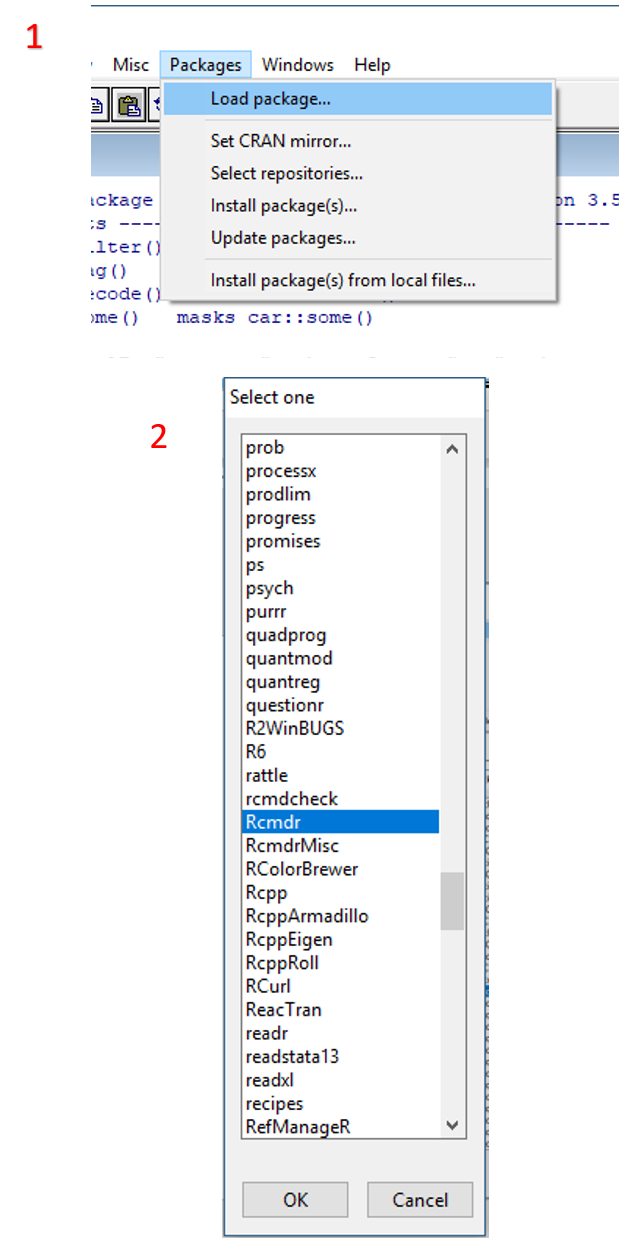
\includegraphics[width=0.7\linewidth]{./images/chp1/loadrcmdr} 

}

\caption{Tampilan proses pemuatan paket Rcmdr.}\label{fig:loadrcmdr}
\end{figure}

\hypertarget{tampilan-r-dan-r-commander}{%
\section{\texorpdfstring{Tampilan \texttt{R} dan \texttt{R\ Commander}}{Tampilan R dan R Commander}}\label{tampilan-r-dan-r-commander}}

\hypertarget{antarmuka-r}{%
\subsection{\texorpdfstring{Antarmuka \texttt{R}}{Antarmuka R}}\label{antarmuka-r}}

Tampilan \texttt{R} saat pertama kali dilankan dapat dilihat seperti pada Gambar \ref{fig:tampilanr}. Pada Gambar tersebut, jendela \texttt{R} terbagi menjadi 4 bagian, antara lain:

\begin{figure}

{\centering 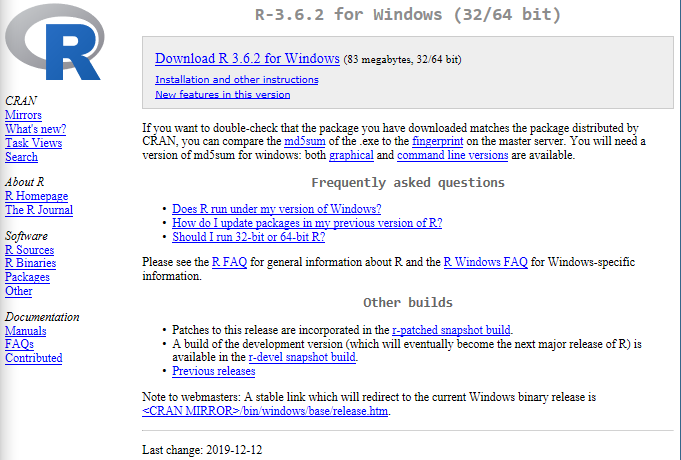
\includegraphics[width=0.8\linewidth]{./images/chp1/rwin} 

}

\caption{Tampilan antar muka jendela R for windows.}\label{fig:tampilanr}
\end{figure}

\textbf{Bagian 1}: baris menu yang terdiri atas menu:

\begin{itemize}
\tightlist
\item
  \textbf{File} : menu yang berkaitan dengan cara membuat dan menyimpan \emph{script} R, memuat dan menyimpan \emph{history} kerja, merubah direktori kerja, mencetak dan menyimpan file, dan keluar dari \texttt{R}.
\item
  \textbf{Edit} : menu yang berkaitan dengan sejumlah perintah untuk melakukan \emph{editing} seperti \emph{copy} dan \emph{paste}, memilih atau meng-\emph{highlight} sejumlah sintaks, membersihkan \emph{R console}, membuka \emph{data editor}, dan perintah untuk membuka jendela pengaturan GUI \texttt{R}.
\item
  \textbf{View} : menu yang memungkinkan pengguna melakukan pengaturan tampilan jendela \texttt{R} seperti menampilkan panel \emph{toolbar} atau menampilkan panel status.
\item
  \textbf{Misc} : menu yang menampilkan sejumlah submenu perintah dan pilihan untuk menghentikan proses komputasi, menampilkan dan menghapus seluruh objek yang telah dibuat, dan menampilkan paket-paket yang aktif.
\item
  \textbf{Packages} : menu yang digunakan untuk mengatur paket-paket yang ada di \texttt{R}, seperti: memuat paket, memasang dan menghapus paket, memperbaharui paket, dan melakukan pengaturan repository berupa lokasi paket-paket yang akan dipasang.
\item
  \textbf{Windows} : menu yang menampilkan fungsi pengaturan jendela-jendela yang ada pada \textbf{Bagian 4}.
\item
  \textbf{Help} : menu bantuan \texttt{R}.
\end{itemize}

Secara lengkap fitur yang tersedia pada baris menu ditampilkan pada diagram pohon menu berikut:

\begin{Shaded}
\begin{Highlighting}[]
\NormalTok{File}
  \OperatorTok{|-}\StringTok{ }\NormalTok{Source R code...}
  \OperatorTok{|-}\StringTok{ }\NormalTok{New script...}
  \OperatorTok{|-}\StringTok{ }\NormalTok{Open script...}
  \OperatorTok{|-}\StringTok{ }\NormalTok{Display }\KeywordTok{file}\NormalTok{(s)...}
  \OperatorTok{|-}\StringTok{ }\NormalTok{Load Workspace...}
  \OperatorTok{|-}\StringTok{ }\NormalTok{Save Workspace...}
  \OperatorTok{|-}\StringTok{ }\NormalTok{Load History...}
  \OperatorTok{|-}\StringTok{ }\NormalTok{Save History...}
  \OperatorTok{|-}\StringTok{ }\NormalTok{Change dir...}
  \OperatorTok{|-}\StringTok{ }\NormalTok{Print...}
  \OperatorTok{|-}\StringTok{ }\NormalTok{Save to File...}
  \OperatorTok{|-}\StringTok{ }\NormalTok{Exit}
\NormalTok{Edit}
  \OperatorTok{|-}\StringTok{ }\NormalTok{Copy}
  \OperatorTok{|-}\StringTok{ }\NormalTok{Paste}
  \OperatorTok{|-}\StringTok{ }\NormalTok{Paste commands only}
  \OperatorTok{|-}\StringTok{ }\NormalTok{Copy and Paste}
  \OperatorTok{|-}\StringTok{ }\NormalTok{Select all}
  \OperatorTok{|-}\StringTok{ }\NormalTok{Clear console}
  \OperatorTok{|-}\StringTok{ }\NormalTok{Data editor}
  \OperatorTok{|-}\StringTok{ }\NormalTok{GUI preferences}
\NormalTok{View}
  \OperatorTok{|-}\StringTok{ }\NormalTok{Toolbar}
  \OperatorTok{|-}\StringTok{ }\NormalTok{Statusbar}
\NormalTok{Misc}
  \OperatorTok{|-}\StringTok{ }\NormalTok{Stop current computation}
  \OperatorTok{|-}\StringTok{ }\NormalTok{Stop all computations}
  \OperatorTok{|-}\StringTok{ }\NormalTok{Buffered output}
  \OperatorTok{|-}\StringTok{ }\NormalTok{Word completion}
  \OperatorTok{|-}\StringTok{ }\NormalTok{Filename completion}
  \OperatorTok{|-}\StringTok{ }\NormalTok{List objects}
  \OperatorTok{|-}\StringTok{ }\NormalTok{Remove all objects}
  \OperatorTok{|-}\StringTok{ }\NormalTok{List search path}
\NormalTok{Packages}
  \OperatorTok{|-}\StringTok{ }\NormalTok{Load package...}
  \OperatorTok{|-}\StringTok{ }\NormalTok{Set CRAN mirror...}
  \OperatorTok{|-}\StringTok{ }\NormalTok{Select repositories...}
  \OperatorTok{|-}\StringTok{ }\NormalTok{Install }\KeywordTok{package}\NormalTok{(s)...}
  \OperatorTok{|-}\StringTok{ }\NormalTok{Update }\KeywordTok{package}\NormalTok{(s)...}
  \OperatorTok{|-}\StringTok{ }\NormalTok{Install }\KeywordTok{package}\NormalTok{(s) from local files...}
\NormalTok{Misc}
  \OperatorTok{|-}\StringTok{ }\NormalTok{Cascade}
  \OperatorTok{|-}\StringTok{ }\NormalTok{Tile Horizontally}
  \OperatorTok{|-}\StringTok{ }\NormalTok{Tile Vertically}
  \OperatorTok{|-}\StringTok{ }\NormalTok{Arrange Icons}
\NormalTok{Help}
  \OperatorTok{|-}\StringTok{ }\NormalTok{Console}
  \OperatorTok{|-}\StringTok{ }\NormalTok{FAQ on R}
  \OperatorTok{|-}\StringTok{ }\NormalTok{FAQ on R }\ControlFlowTok{for}\NormalTok{ Windosw}
  \OperatorTok{|-}\StringTok{ }\KeywordTok{Manuals}\NormalTok{ (}\ControlFlowTok{in}\NormalTok{ PDF)}
  \OperatorTok{|}\StringTok{ }\ErrorTok{|}\OperatorTok{-}\StringTok{ }\NormalTok{An Introduction tor R}
  \OperatorTok{|}\StringTok{ }\ErrorTok{|}\OperatorTok{-}\StringTok{ }\NormalTok{R reference}
  \OperatorTok{|}\StringTok{ }\ErrorTok{|}\OperatorTok{-}\StringTok{ }\NormalTok{R Data Import}\OperatorTok{/}\NormalTok{Export}
  \OperatorTok{|}\StringTok{ }\ErrorTok{|}\OperatorTok{-}\StringTok{ }\NormalTok{R Language Definition}
  \OperatorTok{|}\StringTok{ }\ErrorTok{|}\OperatorTok{-}\StringTok{ }\NormalTok{Writing R Extensions}
  \OperatorTok{|}\StringTok{ }\ErrorTok{|}\OperatorTok{-}\StringTok{ }\NormalTok{R Internals}
  \OperatorTok{|}\StringTok{ }\ErrorTok{|}\OperatorTok{-}\StringTok{ }\NormalTok{R Installation and Administration}
  \OperatorTok{|}\StringTok{ }\ErrorTok{|}\OperatorTok{-}\StringTok{ }\NormalTok{Sweave User}
  \OperatorTok{|-}\StringTok{ }\NormalTok{R }\KeywordTok{functions}\NormalTok{ (text)...}
  \OperatorTok{|-}\StringTok{ }\NormalTok{Html help}
  \OperatorTok{|-}\StringTok{ }\NormalTok{Search help...}
  \OperatorTok{|-}\StringTok{ }\NormalTok{search.r}\OperatorTok{-}\NormalTok{project.org...}
  \OperatorTok{|-}\StringTok{ }\NormalTok{Apropos...}
  \OperatorTok{|-}\StringTok{ }\NormalTok{R Project home page}
  \OperatorTok{|-}\StringTok{ }\NormalTok{CRAN home page}
  \OperatorTok{|-}\StringTok{ }\NormalTok{About}
\end{Highlighting}
\end{Shaded}

\textbf{Bagian 2} : panel yang berisikan \emph{toolbar} untuk membuka \emph{R script}, memuat dan menyimpan ruang kerja, perintah \emph{copy and paste}, menghentikan komputasi, dan mencetak hasil perhitungan pada jendela \emph{console} dan editor.

\textbf{Bagian 3} : jendela \emph{console}.

\textbf{Bagian 4} : ruang kosong lokasi jendela baru seperti \emph{console} dan grafik dimuat.

\hypertarget{antarmuka-r-commander}{%
\subsection{\texorpdfstring{Antarmuka \texttt{R\ Commander}}{Antarmuka R Commander}}\label{antarmuka-r-commander}}

Tampilan \texttt{R\ Commander} saat pertama kali dijalankan dapat dilihat seperti pada Gambar \ref{fig:tampilanrcmdr}. Pada Gambar tersebut, jendela \texttt{R\ Commander} terbagi menjadi 5 bagian, antara lain:

\begin{figure}

{\centering 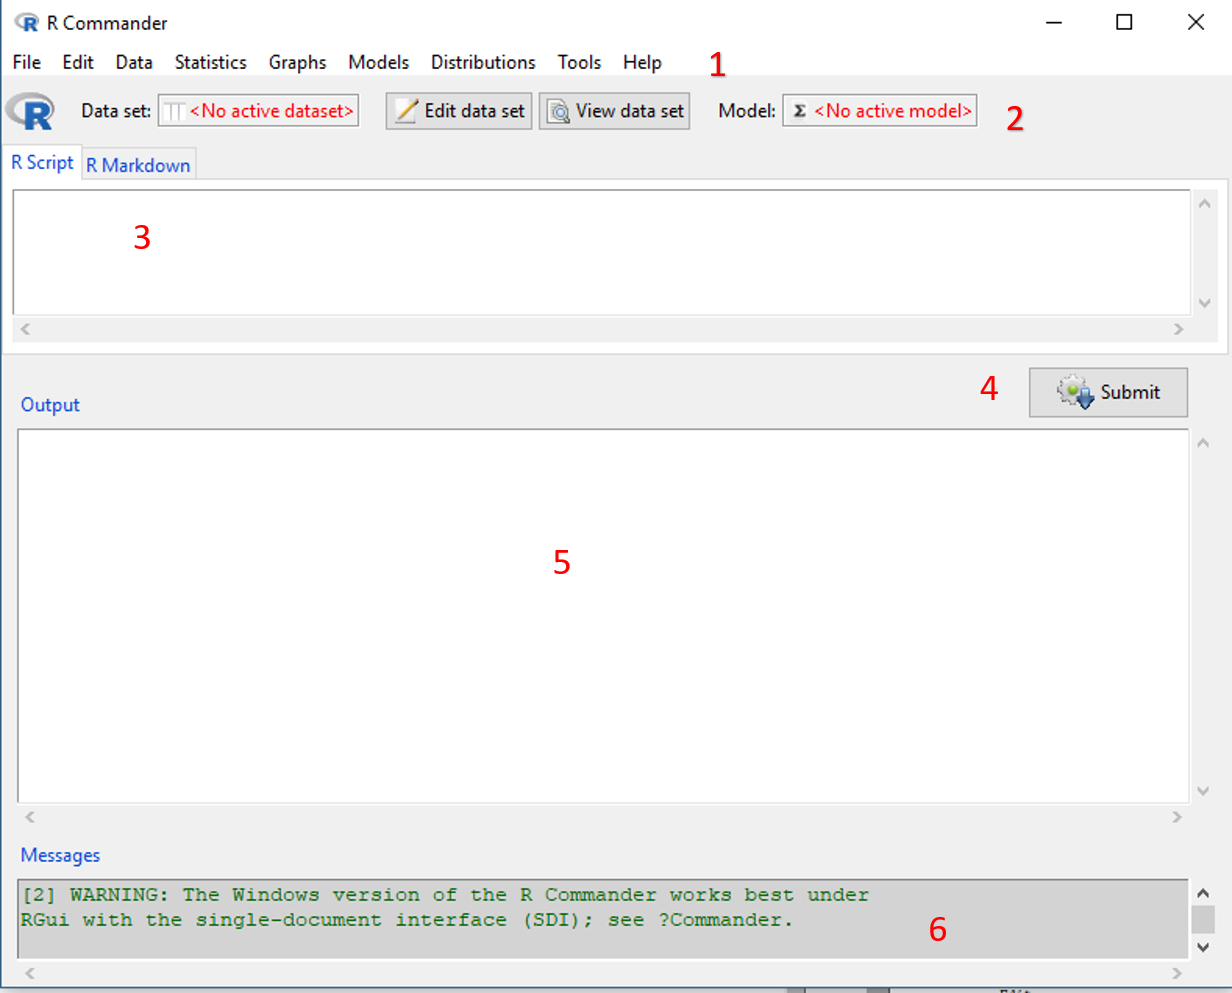
\includegraphics[width=0.8\linewidth]{./images/chp1/tampilan_rcmdr} 

}

\caption{Tampilan antar muka jendela R Commander.}\label{fig:tampilanrcmdr}
\end{figure}

\textbf{Bagian 1} : baris menu yang terdiri atas menu:

\begin{itemize}
\tightlist
\item
  \textbf{File} : menu untuk memuat dan menyimpan file \emph{script}, menyimpan \emph{output} dan ruang kerja \texttt{R}; dan keluar dari \texttt{R\ Commander} atau dari \texttt{R} dan \texttt{R\ Commander}.
\item
  \textbf{Edit} : menu (\emph{cut}, \emph{copy}, \emph{paste}, dll.) Untuk mengedit teks di berbagai panel dan tab. Mengklik kanan di salah satu panel atau tab ini juga memunculkan menu edit sesuai dengan tab yang digunakan.
\item
  \textbf{Data} : menu yang terdiri atas submenu untuk membaca dan mengolah data.
\item
  \textbf{Statistics} : menu yang terdiri atas berbagai submenu untuk melakukan berbagai analisis statistik.
\item
  \textbf{Graphs} : menu yang terdiri atas submenu yang berisikan berbagai metode visualisasi data.
\item
  \textbf{Models} : menu dan submenu yang digunakan untuk memperoleh ringkasan numerik, rentang keyakinan, uji hipotesis, diagnosa, dan grafik dari model statistik, dan menambahkan hasil diagnosa pada dataset seperti menambahkan residu atau error model pada dataset.
\item
  \textbf{Distribution} : menu yang terdiri atas submenu yang digunakan untuk memperoleh probabilitas kumulatif, densitas probabilitas, kuantil, dan grafik dari distribusi statistika standar.
\item
  \textbf{Tools} : menu yang digunakan untuk mengakses paket \texttt{R} (contoh: memuat dataset dari paket lainnya, memuat paket untuk menambahkan metode analisis statistik, dll), untuk memuat paket \texttt{Rcmdr\ plug-in}, mengatur sebagian besar opsi pada \texttt{R\ Commander}, dan untuk memasang \emph{optional auxilary software}.
\item
  \textbf{Help} : menu bantuan yang berguna untuk memperoleh informasi terkait \texttt{R\ Commander} dan paket terkait lainnya.
\end{itemize}

Secara lengkap menu dan submenu pada \texttt{R\ Commander} ditampilkan pada diagram pohon berikut:

\begin{Shaded}
\begin{Highlighting}[]
\NormalTok{File}
  \OperatorTok{|-}\StringTok{ }\NormalTok{Change working directory...}
  \OperatorTok{|-}\StringTok{ }\NormalTok{Open script file...}
  \OperatorTok{|-}\StringTok{ }\NormalTok{Save script...}
  \OperatorTok{|-}\StringTok{ }\NormalTok{Save script as...}
  \OperatorTok{|-}\StringTok{ }\NormalTok{Open R Markdown file...}
  \OperatorTok{|-}\StringTok{ }\NormalTok{Save R Markdown file...}
  \OperatorTok{|-}\StringTok{ }\NormalTok{Save R Markdown file as...}
  \OperatorTok{|-}\StringTok{ }\NormalTok{Save output...}
  \OperatorTok{|-}\StringTok{ }\NormalTok{Save output as...}
  \OperatorTok{|-}\StringTok{ }\NormalTok{Save R workspace...}
  \OperatorTok{|-}\StringTok{ }\NormalTok{Save R workspace as...}
  \OperatorTok{|-}\StringTok{ }\NormalTok{Exit}
  \OperatorTok{|}\StringTok{ }\ErrorTok{|}\OperatorTok{-}\StringTok{ }\NormalTok{From Commander}
  \OperatorTok{|}\StringTok{ }\ErrorTok{|}\OperatorTok{-}\StringTok{ }\NormalTok{From Commander and R}
\NormalTok{Edit}
  \OperatorTok{|-}\StringTok{ }\NormalTok{Edit R Markdown document}
  \OperatorTok{|-}\StringTok{ }\NormalTok{Edit knitr document}
  \OperatorTok{|-}\StringTok{ }\NormalTok{Remove last Markdown command block}
  \OperatorTok{|-}\StringTok{ }\NormalTok{Remove last knitr command block}
  \OperatorTok{|-}\StringTok{ }\NormalTok{Cut}
  \OperatorTok{|-}\StringTok{ }\NormalTok{Copy}
  \OperatorTok{|-}\StringTok{ }\NormalTok{Paste}
  \OperatorTok{|-}\StringTok{ }\NormalTok{Delete}
  \OperatorTok{|-}\StringTok{ }\NormalTok{Find}
  \OperatorTok{|-}\StringTok{ }\NormalTok{Select all}
  \OperatorTok{|-}\StringTok{ }\NormalTok{Undo}
  \OperatorTok{|-}\StringTok{ }\NormalTok{Redo}
  \OperatorTok{|-}\StringTok{ }\NormalTok{Clear window}
\NormalTok{Data}
  \OperatorTok{|-}\StringTok{ }\NormalTok{New data set...}
  \OperatorTok{|-}\StringTok{ }\NormalTok{Load data set...}
  \OperatorTok{|-}\StringTok{ }\NormalTok{Merge data sets...}
  \OperatorTok{|-}\StringTok{ }\NormalTok{Import data}
  \OperatorTok{|}\StringTok{ }\ErrorTok{|}\OperatorTok{-}\StringTok{ }\NormalTok{from text file, clipboard, or URL...}
  \OperatorTok{|}\StringTok{ }\ErrorTok{|}\OperatorTok{-}\StringTok{ }\NormalTok{from SPSS data set...}
  \OperatorTok{|}\StringTok{ }\ErrorTok{|}\OperatorTok{-}\StringTok{ }\NormalTok{from SAS xport file...}
  \OperatorTok{|}\StringTok{ }\ErrorTok{|}\OperatorTok{-}\StringTok{ }\NormalTok{from SAS b7dat file...}
  \OperatorTok{|}\StringTok{ }\ErrorTok{|}\OperatorTok{-}\StringTok{ }\NormalTok{from Minitab data set...}
  \OperatorTok{|}\StringTok{ }\ErrorTok{|}\OperatorTok{-}\StringTok{ }\NormalTok{from STATA data set...}
  \OperatorTok{|}\StringTok{ }\ErrorTok{|}\OperatorTok{-}\StringTok{ }\NormalTok{from Excel file...}
  \OperatorTok{|-}\StringTok{ }\NormalTok{Data }\ControlFlowTok{in}\NormalTok{ packages}
  \OperatorTok{|}\StringTok{ }\ErrorTok{|}\OperatorTok{-}\StringTok{ }\NormalTok{List data sets }\ControlFlowTok{in}\NormalTok{ packages}
  \OperatorTok{|}\StringTok{ }\ErrorTok{|}\OperatorTok{-}\StringTok{ }\NormalTok{Read data set from an attached package...}
  \OperatorTok{|-}\StringTok{ }\NormalTok{Active data set}
  \OperatorTok{|}\StringTok{ }\ErrorTok{|}\OperatorTok{-}\StringTok{ }\NormalTok{View data...}
  \OperatorTok{|}\StringTok{ }\ErrorTok{|}\OperatorTok{-}\StringTok{ }\NormalTok{Select active data set...}
  \OperatorTok{|}\StringTok{ }\ErrorTok{|}\OperatorTok{-}\StringTok{ }\NormalTok{Refresh active data set}
  \OperatorTok{|}\StringTok{ }\ErrorTok{|}\OperatorTok{-}\StringTok{ }\NormalTok{Help on active data }\KeywordTok{set}\NormalTok{ (}\ControlFlowTok{if}\NormalTok{ available)}
  \OperatorTok{|}\StringTok{ }\ErrorTok{|}\OperatorTok{-}\StringTok{ }\NormalTok{Variables }\ControlFlowTok{in}\NormalTok{ active data set}
  \OperatorTok{|}\StringTok{ }\ErrorTok{|}\OperatorTok{-}\StringTok{ }\NormalTok{Set case names...}
  \OperatorTok{|}\StringTok{ }\ErrorTok{|}\OperatorTok{-}\StringTok{ }\NormalTok{Subset active data set...}
  \OperatorTok{|}\StringTok{ }\ErrorTok{|}\OperatorTok{-}\StringTok{ }\NormalTok{Sort active data set...}
  \OperatorTok{|}\StringTok{ }\ErrorTok{|}\OperatorTok{-}\StringTok{ }\NormalTok{Aggregate variables }\ControlFlowTok{in}\NormalTok{ active data set...}
  \OperatorTok{|}\StringTok{ }\ErrorTok{|}\OperatorTok{-}\StringTok{ }\NormalTok{Remove }\KeywordTok{row}\NormalTok{(s) from active data set...}
  \OperatorTok{|}\StringTok{ }\ErrorTok{|}\OperatorTok{-}\StringTok{ }\NormalTok{Stack variables }\ControlFlowTok{in}\NormalTok{ active data set...}
  \OperatorTok{|}\StringTok{ }\ErrorTok{|}\OperatorTok{-}\StringTok{ }\NormalTok{Remove cases with missing data...}
  \OperatorTok{|}\StringTok{ }\ErrorTok{|}\OperatorTok{-}\StringTok{ }\NormalTok{Save active data set...}
  \OperatorTok{|}\StringTok{ }\ErrorTok{|}\OperatorTok{-}\StringTok{ }\NormalTok{Export active data set...}
  \OperatorTok{|-}\StringTok{ }\NormalTok{Manage variables }\ControlFlowTok{in}\NormalTok{ active data set}
  \OperatorTok{|}\StringTok{ }\ErrorTok{|}\OperatorTok{-}\StringTok{ }\NormalTok{Recode variable...}
  \OperatorTok{|}\StringTok{ }\ErrorTok{|}\OperatorTok{-}\StringTok{ }\NormalTok{Compute new variable...}
  \OperatorTok{|}\StringTok{ }\ErrorTok{|}\OperatorTok{-}\StringTok{ }\NormalTok{Add observation numbers to data set}
  \OperatorTok{|}\StringTok{ }\ErrorTok{|}\OperatorTok{-}\StringTok{ }\NormalTok{Standardize variables...}
  \OperatorTok{|}\StringTok{ }\ErrorTok{|}\OperatorTok{-}\StringTok{ }\NormalTok{Convert numeric variables to factors...}
  \OperatorTok{|}\StringTok{ }\ErrorTok{|}\OperatorTok{-}\StringTok{ }\NormalTok{Bin numeric variable...}
  \OperatorTok{|}\StringTok{ }\ErrorTok{|}\OperatorTok{-}\StringTok{ }\NormalTok{Reorder factor levels...}
  \OperatorTok{|}\StringTok{ }\ErrorTok{|}\OperatorTok{-}\StringTok{ }\NormalTok{Drop unused factor levels...}
  \OperatorTok{|}\StringTok{ }\ErrorTok{|}\OperatorTok{-}\StringTok{ }\NormalTok{Define contrasts }\ControlFlowTok{for}\NormalTok{ a factor...}
  \OperatorTok{|}\StringTok{ }\ErrorTok{|}\OperatorTok{-}\StringTok{ }\NormalTok{Rename variables...}
  \OperatorTok{|}\StringTok{ }\ErrorTok{|}\OperatorTok{-}\StringTok{ }\NormalTok{Delete variables from data set ...}
\NormalTok{Statistics}
  \OperatorTok{|-}\StringTok{ }\NormalTok{Summaries}
  \OperatorTok{|}\StringTok{ }\ErrorTok{|}\OperatorTok{-}\StringTok{ }\NormalTok{Active data set}
  \OperatorTok{|}\StringTok{ }\ErrorTok{|}\OperatorTok{-}\StringTok{ }\NormalTok{Numerical summaries...}
  \OperatorTok{|}\StringTok{ }\ErrorTok{|}\OperatorTok{-}\StringTok{ }\NormalTok{Frequency distributions...}
  \OperatorTok{|}\StringTok{ }\ErrorTok{|}\OperatorTok{-}\StringTok{ }\NormalTok{Count missing observations}
  \OperatorTok{|}\StringTok{ }\ErrorTok{|}\OperatorTok{-}\StringTok{ }\NormalTok{Table of statistics...}
  \OperatorTok{|}\StringTok{ }\ErrorTok{|}\OperatorTok{-}\StringTok{ }\NormalTok{Correlation matrix...}
  \OperatorTok{|}\StringTok{ }\ErrorTok{|}\OperatorTok{-}\StringTok{ }\NormalTok{Correlation test...}
  \OperatorTok{|}\StringTok{ }\ErrorTok{|}\OperatorTok{-}\StringTok{ }\NormalTok{Test of normality...}
  \OperatorTok{|}\StringTok{ }\ErrorTok{|}\OperatorTok{-}\StringTok{ }\NormalTok{Transform toward normality...}
  \OperatorTok{|-}\NormalTok{Contingency tables}
  \OperatorTok{|}\StringTok{ }\ErrorTok{|}\OperatorTok{-}\StringTok{ }\NormalTok{Two}\OperatorTok{-}\NormalTok{way table...}
  \OperatorTok{|}\StringTok{ }\ErrorTok{|}\OperatorTok{-}\StringTok{ }\NormalTok{Multi}\OperatorTok{-}\NormalTok{way table...}
  \OperatorTok{|}\StringTok{ }\ErrorTok{|}\OperatorTok{-}\StringTok{ }\NormalTok{Enter and analyze two}\OperatorTok{-}\NormalTok{way table...}
  \OperatorTok{|-}\StringTok{ }\NormalTok{Means}
  \OperatorTok{|}\StringTok{ }\ErrorTok{|}\OperatorTok{-}\StringTok{ }\NormalTok{Single}\OperatorTok{-}\NormalTok{sample t}\OperatorTok{-}\NormalTok{test...}
  \OperatorTok{|}\StringTok{ }\ErrorTok{|}\OperatorTok{-}\StringTok{ }\NormalTok{Independent samples t}\OperatorTok{-}\NormalTok{test...}
  \OperatorTok{|}\StringTok{ }\ErrorTok{|}\OperatorTok{-}\StringTok{ }\NormalTok{Paired t}\OperatorTok{-}\NormalTok{test...}
  \OperatorTok{|}\StringTok{ }\ErrorTok{|}\OperatorTok{-}\StringTok{ }\NormalTok{One}\OperatorTok{-}\NormalTok{way ANOVA...}
  \OperatorTok{|}\StringTok{ }\ErrorTok{|}\OperatorTok{-}\StringTok{ }\NormalTok{Multi}\OperatorTok{-}\NormalTok{way ANOVA...}
  \OperatorTok{|-}\StringTok{ }\NormalTok{Proportions}
  \OperatorTok{|}\StringTok{ }\ErrorTok{|}\OperatorTok{-}\StringTok{ }\NormalTok{Single}\OperatorTok{-}\NormalTok{sample proportion test...}
  \OperatorTok{|}\StringTok{ }\ErrorTok{|}\OperatorTok{-}\StringTok{ }\NormalTok{Two}\OperatorTok{-}\NormalTok{sample proportions test...}
  \OperatorTok{|-}\StringTok{ }\NormalTok{Variances}
  \OperatorTok{|}\StringTok{ }\ErrorTok{|}\OperatorTok{-}\StringTok{ }\NormalTok{Two}\OperatorTok{-}\NormalTok{variances F}\OperatorTok{-}\NormalTok{test...}
  \OperatorTok{|}\StringTok{ }\ErrorTok{|}\OperatorTok{-}\StringTok{ }\NormalTok{Bartlett}\StringTok{'s test...}
\StringTok{  | |- Levene'}\NormalTok{s test...}
  \OperatorTok{|-}\StringTok{ }\NormalTok{Nonparametric tests}
  \OperatorTok{|}\StringTok{ }\ErrorTok{|}\OperatorTok{-}\StringTok{ }\NormalTok{Two}\OperatorTok{-}\NormalTok{sample Wilcoxon test...}
  \OperatorTok{|}\StringTok{ }\ErrorTok{|}\OperatorTok{-}\StringTok{ }\NormalTok{Single}\OperatorTok{-}\NormalTok{sample Wilcoxon test...}
  \OperatorTok{|}\StringTok{ }\ErrorTok{|}\OperatorTok{-}\StringTok{ }\NormalTok{Paired}\OperatorTok{-}\NormalTok{samples Wilcoxon test...}
  \OperatorTok{|}\StringTok{ }\ErrorTok{|}\OperatorTok{-}\StringTok{ }\NormalTok{Kruskal}\OperatorTok{-}\NormalTok{Wallis test...}
  \OperatorTok{|}\StringTok{ }\ErrorTok{|}\OperatorTok{-}\StringTok{ }\NormalTok{Friedman rank}\OperatorTok{-}\NormalTok{sum test...}
  \OperatorTok{|-}\StringTok{ }\NormalTok{Dimensional analysis}
  \OperatorTok{|}\StringTok{ }\ErrorTok{|}\OperatorTok{-}\StringTok{ }\NormalTok{Scale reliability...}
  \OperatorTok{|}\StringTok{ }\ErrorTok{|}\OperatorTok{-}\StringTok{ }\NormalTok{Principal}\OperatorTok{-}\NormalTok{components analysis...}
  \OperatorTok{|}\StringTok{ }\ErrorTok{|}\OperatorTok{-}\StringTok{ }\NormalTok{Factor analysis...}
  \OperatorTok{|}\StringTok{ }\ErrorTok{|}\OperatorTok{-}\StringTok{ }\NormalTok{Confirmatory factor analysis...}
  \OperatorTok{|}\StringTok{ }\ErrorTok{|}\OperatorTok{-}\StringTok{ }\NormalTok{Cluster analysis}
  \OperatorTok{|}\StringTok{ }\ErrorTok{|}\StringTok{ }\ErrorTok{|}\OperatorTok{-}\StringTok{ }\NormalTok{k}\OperatorTok{-}\NormalTok{means cluster analysis...}
  \OperatorTok{|}\StringTok{ }\ErrorTok{|}\StringTok{ }\ErrorTok{|}\OperatorTok{-}\StringTok{ }\NormalTok{Hierarchical cluster analysis...}
  \OperatorTok{|}\StringTok{ }\ErrorTok{|}\StringTok{ }\ErrorTok{|}\OperatorTok{-}\StringTok{ }\NormalTok{Summarize hierarchical clustering...}
  \OperatorTok{|}\StringTok{ }\ErrorTok{|}\StringTok{ }\ErrorTok{|}\OperatorTok{-}\StringTok{ }\NormalTok{Add hierarchical clustering to data set...}
  \OperatorTok{|-}\StringTok{ }\NormalTok{Fit models}
  \OperatorTok{|}\StringTok{ }\ErrorTok{|}\OperatorTok{-}\StringTok{ }\NormalTok{Linear regression...}
  \OperatorTok{|}\StringTok{ }\ErrorTok{|}\OperatorTok{-}\StringTok{ }\NormalTok{Linear model...}
  \OperatorTok{|}\StringTok{ }\ErrorTok{|}\OperatorTok{-}\StringTok{ }\NormalTok{Generalized linear model...}
  \OperatorTok{|}\StringTok{ }\ErrorTok{|}\OperatorTok{-}\StringTok{ }\NormalTok{Multinomial logit model...}
  \OperatorTok{|}\StringTok{ }\ErrorTok{|}\OperatorTok{-}\StringTok{ }\NormalTok{Ordinal regression model...}
\NormalTok{Graphs}
  \OperatorTok{|-}\StringTok{ }\NormalTok{Color palette...}
  \OperatorTok{|-}\StringTok{ }\NormalTok{Index plot...}
  \OperatorTok{|-}\StringTok{ }\NormalTok{Dot plot...}
  \OperatorTok{|-}\StringTok{ }\NormalTok{Histogram...}
  \OperatorTok{|-}\StringTok{ }\NormalTok{Plot discrete numeric variable......}
  \OperatorTok{|-}\StringTok{ }\NormalTok{Density estimate...}
  \OperatorTok{|-}\StringTok{ }\NormalTok{Stem}\OperatorTok{-}\NormalTok{and}\OperatorTok{-}\NormalTok{leaf display...}
  \OperatorTok{|-}\StringTok{ }\NormalTok{Boxplot...}
  \OperatorTok{|-}\StringTok{ }\NormalTok{Quantile}\OperatorTok{-}\NormalTok{comparison plot...}
  \OperatorTok{|-}\StringTok{ }\NormalTok{Symmetry boxplot...}
  \OperatorTok{|-}\StringTok{ }\NormalTok{Scatterplot...}
  \OperatorTok{|-}\StringTok{ }\NormalTok{Scatterplot matrix...}
  \OperatorTok{|-}\StringTok{ }\NormalTok{Line graph...}
  \OperatorTok{|-}\StringTok{ }\NormalTok{XY conditioning plot...}
  \OperatorTok{|-}\StringTok{ }\NormalTok{Plot of means...}
  \OperatorTok{|-}\StringTok{ }\NormalTok{Strip chart...}
  \OperatorTok{|-}\StringTok{ }\NormalTok{Bar graph...}
  \OperatorTok{|-}\StringTok{ }\NormalTok{Pie chart...}
  \OperatorTok{|-}\StringTok{ }\NormalTok{3D graph}
  \OperatorTok{|}\StringTok{ }\ErrorTok{|}\OperatorTok{-}\StringTok{ }\NormalTok{3D scatterplot...}
  \OperatorTok{|}\StringTok{ }\ErrorTok{|}\OperatorTok{-}\StringTok{ }\NormalTok{Identify observations with mouse}
  \OperatorTok{|}\StringTok{ }\ErrorTok{|}\OperatorTok{-}\StringTok{ }\NormalTok{Save graph to file}
  \OperatorTok{|-}\StringTok{ }\NormalTok{Save graph to file}
  \OperatorTok{|}\StringTok{ }\ErrorTok{|}\OperatorTok{-}\StringTok{ }\NormalTok{as bitmap...}
  \OperatorTok{|}\StringTok{ }\ErrorTok{|}\OperatorTok{-}\StringTok{ }\NormalTok{as PDF}\OperatorTok{/}\NormalTok{Postscript}\OperatorTok{/}\NormalTok{EPS...}
  \OperatorTok{|}\StringTok{ }\ErrorTok{|}\OperatorTok{-}\StringTok{ }\NormalTok{3D RGL graph...}
\NormalTok{Models}
  \OperatorTok{|-}\StringTok{ }\NormalTok{Select active model...}
  \OperatorTok{|-}\StringTok{ }\NormalTok{Summarize model}
  \OperatorTok{|-}\StringTok{ }\NormalTok{Compare model coefficients...}
  \OperatorTok{|-}\StringTok{ }\NormalTok{Add observation statistics to data...}
  \OperatorTok{|-}\StringTok{ }\NormalTok{Akaike Information }\KeywordTok{Criterion}\NormalTok{ (AIC)}
  \OperatorTok{|-}\StringTok{ }\NormalTok{Bayesian Information }\KeywordTok{Criterion}\NormalTok{ (BIC)}
  \OperatorTok{|-}\StringTok{ }\NormalTok{Stepwise model selection...}
  \OperatorTok{|-}\StringTok{ }\NormalTok{Subset model selection...}
  \OperatorTok{|-}\StringTok{ }\NormalTok{Confidence intervals......}
  \OperatorTok{|-}\StringTok{ }\NormalTok{Bootstrap confidence intervals...}
  \OperatorTok{|-}\StringTok{ }\NormalTok{Delta method confidence interval...}
  \OperatorTok{|-}\StringTok{ }\NormalTok{Hypothesis tests}
  \OperatorTok{|}\StringTok{ }\ErrorTok{|}\OperatorTok{-}\StringTok{ }\NormalTok{ANOVA table...}
  \OperatorTok{|}\StringTok{ }\ErrorTok{|}\OperatorTok{-}\StringTok{ }\NormalTok{Compare two models...}
  \OperatorTok{|}\StringTok{ }\ErrorTok{|}\OperatorTok{-}\StringTok{ }\NormalTok{Linear hypothesis...}
  \OperatorTok{|-}\StringTok{ }\NormalTok{Numerical diagnostics}
  \OperatorTok{|}\StringTok{ }\ErrorTok{|}\OperatorTok{-}\StringTok{ }\NormalTok{Variance}\OperatorTok{-}\NormalTok{inflation factors}
  \OperatorTok{|}\StringTok{ }\ErrorTok{|}\OperatorTok{-}\StringTok{ }\NormalTok{Breusch}\OperatorTok{-}\NormalTok{Pagan test }\ControlFlowTok{for}\NormalTok{ heteroscedasticity...}
  \OperatorTok{|}\StringTok{ }\ErrorTok{|}\OperatorTok{-}\StringTok{ }\NormalTok{Durbin}\OperatorTok{-}\NormalTok{Watson test }\ControlFlowTok{for}\NormalTok{ autocorrelation...}
  \OperatorTok{|}\StringTok{ }\ErrorTok{|}\OperatorTok{-}\StringTok{ }\NormalTok{RESET test }\ControlFlowTok{for}\NormalTok{ nonlinearity...}
  \OperatorTok{|}\StringTok{ }\ErrorTok{|}\OperatorTok{-}\StringTok{ }\NormalTok{Bonferroni outlier test}
  \OperatorTok{|}\StringTok{ }\ErrorTok{|}\OperatorTok{-}\StringTok{ }\NormalTok{Response transformation...}
  \OperatorTok{|-}\StringTok{ }\NormalTok{Graphs}
  \OperatorTok{|}\StringTok{ }\ErrorTok{|}\OperatorTok{-}\StringTok{ }\NormalTok{Basic diagnostic plots}
  \OperatorTok{|}\StringTok{ }\ErrorTok{|}\OperatorTok{-}\StringTok{ }\NormalTok{Residual quantile}\OperatorTok{-}\NormalTok{comparison plot...}
  \OperatorTok{|}\StringTok{ }\ErrorTok{|}\OperatorTok{-}\StringTok{ }\NormalTok{Component}\OperatorTok{+}\NormalTok{residual plots...}
  \OperatorTok{|}\StringTok{ }\ErrorTok{|}\OperatorTok{-}\StringTok{ }\NormalTok{Added}\OperatorTok{-}\NormalTok{variable plots...}
  \OperatorTok{|}\StringTok{ }\ErrorTok{|}\OperatorTok{-}\StringTok{ }\NormalTok{Influence plot...}
  \OperatorTok{|}\StringTok{ }\ErrorTok{|}\OperatorTok{-}\StringTok{ }\NormalTok{Effect plots...}
  \OperatorTok{|}\StringTok{ }\ErrorTok{|}\OperatorTok{-}\StringTok{ }\NormalTok{Predictor effect plots...}
\NormalTok{Distributions}
  \OperatorTok{|-}\StringTok{ }\NormalTok{Set random number generator seed...}
  \OperatorTok{|-}\StringTok{ }\NormalTok{Continuous distributions}
  \OperatorTok{|}\StringTok{ }\ErrorTok{|}\OperatorTok{-}\StringTok{ }\NormalTok{Normal distribution}
  \OperatorTok{|}\StringTok{ }\ErrorTok{|}\StringTok{ }\ErrorTok{|}\OperatorTok{-}\StringTok{ }\NormalTok{Normal quantiles...}
  \OperatorTok{|}\StringTok{ }\ErrorTok{|}\StringTok{ }\ErrorTok{|}\OperatorTok{-}\StringTok{ }\NormalTok{Normal probabilities...}
  \OperatorTok{|}\StringTok{ }\ErrorTok{|}\StringTok{ }\ErrorTok{|}\OperatorTok{-}\StringTok{ }\NormalTok{Plot normal distribution...}
  \OperatorTok{|}\StringTok{ }\ErrorTok{|}\StringTok{ }\ErrorTok{|}\OperatorTok{-}\StringTok{ }\NormalTok{Sample from normal distribution...}
  \OperatorTok{|}\StringTok{ }\ErrorTok{|}\OperatorTok{-}\StringTok{ }\NormalTok{t distribution}
  \OperatorTok{|}\StringTok{ }\ErrorTok{|}\StringTok{ }\ErrorTok{|}\OperatorTok{-}\StringTok{ }\NormalTok{t quantiles...}
  \OperatorTok{|}\StringTok{ }\ErrorTok{|}\StringTok{ }\ErrorTok{|}\OperatorTok{-}\StringTok{ }\NormalTok{t probabilities...}
  \OperatorTok{|}\StringTok{ }\ErrorTok{|}\StringTok{ }\ErrorTok{|}\OperatorTok{-}\StringTok{ }\NormalTok{Plot t distribution...}
  \OperatorTok{|}\StringTok{ }\ErrorTok{|}\StringTok{ }\ErrorTok{|}\OperatorTok{-}\StringTok{ }\NormalTok{Sample from t distribution...}
  \OperatorTok{|}\StringTok{ }\ErrorTok{|}\OperatorTok{-}\StringTok{ }\NormalTok{Chi}\OperatorTok{-}\NormalTok{squared distribution}
  \OperatorTok{|}\StringTok{ }\ErrorTok{|}\StringTok{ }\ErrorTok{|}\OperatorTok{-}\StringTok{ }\NormalTok{Chi}\OperatorTok{-}\NormalTok{squared quantiles...}
  \OperatorTok{|}\StringTok{ }\ErrorTok{|}\StringTok{ }\ErrorTok{|}\OperatorTok{-}\StringTok{ }\NormalTok{Chi}\OperatorTok{-}\NormalTok{squared probabilities...}
  \OperatorTok{|}\StringTok{ }\ErrorTok{|}\StringTok{ }\ErrorTok{|}\OperatorTok{-}\StringTok{ }\NormalTok{Plot chi}\OperatorTok{-}\NormalTok{squared distribution...}
  \OperatorTok{|}\StringTok{ }\ErrorTok{|}\StringTok{ }\ErrorTok{|}\OperatorTok{-}\StringTok{ }\NormalTok{Sample from chi}\OperatorTok{-}\NormalTok{squared distribution...}
  \OperatorTok{|}\StringTok{ }\ErrorTok{|}\OperatorTok{-}\StringTok{ }\NormalTok{F distribution}
  \OperatorTok{|}\StringTok{ }\ErrorTok{|}\StringTok{ }\ErrorTok{|}\OperatorTok{-}\StringTok{ }\NormalTok{F quantiles...}
  \OperatorTok{|}\StringTok{ }\ErrorTok{|}\StringTok{ }\ErrorTok{|}\OperatorTok{-}\StringTok{ }\NormalTok{F probabilities...}
  \OperatorTok{|}\StringTok{ }\ErrorTok{|}\StringTok{ }\ErrorTok{|}\OperatorTok{-}\StringTok{ }\NormalTok{Plot F distribution...}
  \OperatorTok{|}\StringTok{ }\ErrorTok{|}\StringTok{ }\ErrorTok{|}\OperatorTok{-}\StringTok{ }\NormalTok{Sample from F distribution...}
  \OperatorTok{|}\StringTok{ }\ErrorTok{|}\OperatorTok{-}\StringTok{ }\NormalTok{Exponential distribution}
  \OperatorTok{|}\StringTok{ }\ErrorTok{|}\StringTok{ }\ErrorTok{|}\OperatorTok{-}\StringTok{ }\NormalTok{Exponential quantiles...}
  \OperatorTok{|}\StringTok{ }\ErrorTok{|}\StringTok{ }\ErrorTok{|}\OperatorTok{-}\StringTok{ }\NormalTok{Exponential probabilities...}
  \OperatorTok{|}\StringTok{ }\ErrorTok{|}\StringTok{ }\ErrorTok{|}\OperatorTok{-}\StringTok{ }\NormalTok{Plot exponential distribution...}
  \OperatorTok{|}\StringTok{ }\ErrorTok{|}\StringTok{ }\ErrorTok{|}\OperatorTok{-}\StringTok{ }\NormalTok{Sample from exponential distribution...}
  \OperatorTok{|}\StringTok{ }\ErrorTok{|}\OperatorTok{-}\StringTok{ }\NormalTok{Uniform distribution}
  \OperatorTok{|}\StringTok{ }\ErrorTok{|}\StringTok{ }\ErrorTok{|}\OperatorTok{-}\StringTok{ }\NormalTok{Uniform quantiles...}
  \OperatorTok{|}\StringTok{ }\ErrorTok{|}\StringTok{ }\ErrorTok{|}\OperatorTok{-}\StringTok{ }\NormalTok{Uniform probabilities...}
  \OperatorTok{|}\StringTok{ }\ErrorTok{|}\StringTok{ }\ErrorTok{|}\OperatorTok{-}\StringTok{ }\NormalTok{Plot uniform distribution...}
  \OperatorTok{|}\StringTok{ }\ErrorTok{|}\StringTok{ }\ErrorTok{|}\OperatorTok{-}\StringTok{ }\NormalTok{Sample from uniform distribution...}
  \OperatorTok{|}\StringTok{ }\ErrorTok{|}\OperatorTok{-}\StringTok{ }\NormalTok{Beta distribution}
  \OperatorTok{|}\StringTok{ }\ErrorTok{|}\StringTok{ }\ErrorTok{|}\OperatorTok{-}\StringTok{ }\NormalTok{Beta quantiles...}
  \OperatorTok{|}\StringTok{ }\ErrorTok{|}\StringTok{ }\ErrorTok{|}\OperatorTok{-}\StringTok{ }\NormalTok{Beta probabilities...}
  \OperatorTok{|}\StringTok{ }\ErrorTok{|}\StringTok{ }\ErrorTok{|}\OperatorTok{-}\StringTok{ }\NormalTok{Plot beta distribution...}
  \OperatorTok{|}\StringTok{ }\ErrorTok{|}\StringTok{ }\ErrorTok{|}\OperatorTok{-}\StringTok{ }\NormalTok{Sample from beta distribution...}
  \OperatorTok{|}\StringTok{ }\ErrorTok{|}\OperatorTok{-}\StringTok{ }\NormalTok{Cauchy distribution}
  \OperatorTok{|}\StringTok{ }\ErrorTok{|}\StringTok{ }\ErrorTok{|}\OperatorTok{-}\StringTok{ }\NormalTok{Cauchy quantiles...}
  \OperatorTok{|}\StringTok{ }\ErrorTok{|}\StringTok{ }\ErrorTok{|}\OperatorTok{-}\StringTok{ }\NormalTok{Cauchy probabilities...}
  \OperatorTok{|}\StringTok{ }\ErrorTok{|}\StringTok{ }\ErrorTok{|}\OperatorTok{-}\StringTok{ }\NormalTok{Plot Cauchy distribution...}
  \OperatorTok{|}\StringTok{ }\ErrorTok{|}\StringTok{ }\ErrorTok{|}\OperatorTok{-}\StringTok{ }\NormalTok{Sample from Cauchy distribution...}
  \OperatorTok{|}\StringTok{ }\ErrorTok{|}\OperatorTok{-}\StringTok{ }\NormalTok{Logistic distribution}
  \OperatorTok{|}\StringTok{ }\ErrorTok{|}\StringTok{ }\ErrorTok{|}\OperatorTok{-}\StringTok{ }\NormalTok{Logistic quantiles...}
  \OperatorTok{|}\StringTok{ }\ErrorTok{|}\StringTok{ }\ErrorTok{|}\OperatorTok{-}\StringTok{ }\NormalTok{Logistic probabilities...}
  \OperatorTok{|}\StringTok{ }\ErrorTok{|}\StringTok{ }\ErrorTok{|}\OperatorTok{-}\StringTok{ }\NormalTok{Plot logistic distribution...}
  \OperatorTok{|}\StringTok{ }\ErrorTok{|}\StringTok{ }\ErrorTok{|}\OperatorTok{-}\StringTok{ }\NormalTok{Sample from logistic distribution...}
  \OperatorTok{|}\StringTok{ }\ErrorTok{|}\OperatorTok{-}\StringTok{ }\NormalTok{Lognormal distribution}
  \OperatorTok{|}\StringTok{ }\ErrorTok{|}\StringTok{ }\ErrorTok{|}\OperatorTok{-}\StringTok{ }\NormalTok{Lognormal quantiles...}
  \OperatorTok{|}\StringTok{ }\ErrorTok{|}\StringTok{ }\ErrorTok{|}\OperatorTok{-}\StringTok{ }\NormalTok{Lognormal probabilities...}
  \OperatorTok{|}\StringTok{ }\ErrorTok{|}\StringTok{ }\ErrorTok{|}\OperatorTok{-}\StringTok{ }\NormalTok{Plot lognormal distribution...}
  \OperatorTok{|}\StringTok{ }\ErrorTok{|}\StringTok{ }\ErrorTok{|}\OperatorTok{-}\StringTok{ }\NormalTok{Sample from lognormal distribution...}
  \OperatorTok{|}\StringTok{ }\ErrorTok{|}\OperatorTok{-}\StringTok{ }\NormalTok{Gamma distribution}
  \OperatorTok{|}\StringTok{ }\ErrorTok{|}\StringTok{ }\ErrorTok{|}\OperatorTok{-}\StringTok{ }\NormalTok{Gamma quantiles...}
  \OperatorTok{|}\StringTok{ }\ErrorTok{|}\StringTok{ }\ErrorTok{|}\OperatorTok{-}\StringTok{ }\NormalTok{Gamma probabilities...}
  \OperatorTok{|}\StringTok{ }\ErrorTok{|}\StringTok{ }\ErrorTok{|}\OperatorTok{-}\StringTok{ }\NormalTok{Plot gamma distribution...}
  \OperatorTok{|}\StringTok{ }\ErrorTok{|}\StringTok{ }\ErrorTok{|}\OperatorTok{-}\StringTok{ }\NormalTok{Sample from gamma distribution...}
  \OperatorTok{|}\StringTok{ }\ErrorTok{|}\OperatorTok{-}\StringTok{ }\NormalTok{Weibull distribution}
  \OperatorTok{|}\StringTok{ }\ErrorTok{|}\StringTok{ }\ErrorTok{|}\OperatorTok{-}\StringTok{ }\NormalTok{Weibull quantiles...}
  \OperatorTok{|}\StringTok{ }\ErrorTok{|}\StringTok{ }\ErrorTok{|}\OperatorTok{-}\StringTok{ }\NormalTok{Weibull probabilities...}
  \OperatorTok{|}\StringTok{ }\ErrorTok{|}\StringTok{ }\ErrorTok{|}\OperatorTok{-}\StringTok{ }\NormalTok{Plot Weibull distribution...}
  \OperatorTok{|}\StringTok{ }\ErrorTok{|}\StringTok{ }\ErrorTok{|}\OperatorTok{-}\StringTok{ }\NormalTok{Sample from Weibull distribution...}
  \OperatorTok{|}\StringTok{ }\ErrorTok{|}\OperatorTok{-}\StringTok{ }\NormalTok{Gumbel distribution}
  \OperatorTok{|}\StringTok{ }\ErrorTok{|}\StringTok{ }\ErrorTok{|}\OperatorTok{-}\StringTok{ }\NormalTok{Gumbel quantiles...}
  \OperatorTok{|}\StringTok{ }\ErrorTok{|}\StringTok{ }\ErrorTok{|}\OperatorTok{-}\StringTok{ }\NormalTok{Gumbel probabilities...}
  \OperatorTok{|}\StringTok{ }\ErrorTok{|}\StringTok{ }\ErrorTok{|}\OperatorTok{-}\StringTok{ }\NormalTok{Plot Gumbel distribution...}
  \OperatorTok{|}\StringTok{ }\ErrorTok{|}\StringTok{ }\ErrorTok{|}\OperatorTok{-}\StringTok{ }\NormalTok{Sample from Gumbel distribution...}
  \OperatorTok{|-}\StringTok{ }\NormalTok{Discrete distributions}
  \OperatorTok{|}\StringTok{ }\ErrorTok{|}\OperatorTok{-}\StringTok{ }\NormalTok{Binomial distribution}
  \OperatorTok{|}\StringTok{ }\ErrorTok{|}\StringTok{ }\ErrorTok{|}\OperatorTok{-}\StringTok{ }\NormalTok{Binomial quantiles...}
  \OperatorTok{|}\StringTok{ }\ErrorTok{|}\StringTok{ }\ErrorTok{|}\OperatorTok{-}\StringTok{ }\NormalTok{Binomial tail probabilities...}
  \OperatorTok{|}\StringTok{ }\ErrorTok{|}\StringTok{ }\ErrorTok{|}\OperatorTok{-}\StringTok{ }\NormalTok{Binomial probabilities...}
  \OperatorTok{|}\StringTok{ }\ErrorTok{|}\StringTok{ }\ErrorTok{|}\OperatorTok{-}\StringTok{ }\NormalTok{Plot binomial distribution...}
  \OperatorTok{|}\StringTok{ }\ErrorTok{|}\StringTok{ }\ErrorTok{|}\OperatorTok{-}\StringTok{ }\NormalTok{Sample from binomial distribution...}
  \OperatorTok{|}\StringTok{ }\ErrorTok{|}\OperatorTok{-}\StringTok{ }\NormalTok{Poisson distribution}
  \OperatorTok{|}\StringTok{ }\ErrorTok{|}\StringTok{ }\ErrorTok{|}\OperatorTok{-}\StringTok{ }\NormalTok{Poisson quantiles...}
  \OperatorTok{|}\StringTok{ }\ErrorTok{|}\StringTok{ }\ErrorTok{|}\OperatorTok{-}\StringTok{ }\NormalTok{Poisson tail probabilities...}
  \OperatorTok{|}\StringTok{ }\ErrorTok{|}\StringTok{ }\ErrorTok{|}\OperatorTok{-}\StringTok{ }\NormalTok{Poisson probabilities...}
  \OperatorTok{|}\StringTok{ }\ErrorTok{|}\StringTok{ }\ErrorTok{|}\OperatorTok{-}\StringTok{ }\NormalTok{Plot Poisson distribution...}
  \OperatorTok{|}\StringTok{ }\ErrorTok{|}\StringTok{ }\ErrorTok{|}\OperatorTok{-}\StringTok{ }\NormalTok{Sample from Poisson distribution...}
  \OperatorTok{|}\StringTok{ }\ErrorTok{|}\OperatorTok{-}\StringTok{ }\NormalTok{Geometric distribution}
  \OperatorTok{|}\StringTok{ }\ErrorTok{|}\StringTok{ }\ErrorTok{|}\OperatorTok{-}\StringTok{ }\NormalTok{Geometric quantiles...}
  \OperatorTok{|}\StringTok{ }\ErrorTok{|}\StringTok{ }\ErrorTok{|}\OperatorTok{-}\StringTok{ }\NormalTok{Geometric tail probabilities...}
  \OperatorTok{|}\StringTok{ }\ErrorTok{|}\StringTok{ }\ErrorTok{|}\OperatorTok{-}\StringTok{ }\NormalTok{Geometric probabilities...}
  \OperatorTok{|}\StringTok{ }\ErrorTok{|}\StringTok{ }\ErrorTok{|}\OperatorTok{-}\StringTok{ }\NormalTok{Plot geometric distribution...}
  \OperatorTok{|}\StringTok{ }\ErrorTok{|}\StringTok{ }\ErrorTok{|}\OperatorTok{-}\StringTok{ }\NormalTok{Sample from geometric distribution...}
  \OperatorTok{|}\StringTok{ }\ErrorTok{|}\OperatorTok{-}\StringTok{ }\NormalTok{Hypergeometric distribution}
  \OperatorTok{|}\StringTok{ }\ErrorTok{|}\StringTok{ }\ErrorTok{|}\OperatorTok{-}\StringTok{ }\NormalTok{Hypergeometric quantiles...}
  \OperatorTok{|}\StringTok{ }\ErrorTok{|}\StringTok{ }\ErrorTok{|}\OperatorTok{-}\StringTok{ }\NormalTok{Hypergeometric tail probabilities...}
  \OperatorTok{|}\StringTok{ }\ErrorTok{|}\StringTok{ }\ErrorTok{|}\OperatorTok{-}\StringTok{ }\NormalTok{Hypergeometric probabilities...}
  \OperatorTok{|}\StringTok{ }\ErrorTok{|}\StringTok{ }\ErrorTok{|}\OperatorTok{-}\StringTok{ }\NormalTok{Plot hypergeometric distribution...}
  \OperatorTok{|}\StringTok{ }\ErrorTok{|}\StringTok{ }\ErrorTok{|}\OperatorTok{-}\StringTok{ }\NormalTok{Sample from hypergeometric distribution...}
  \OperatorTok{|}\StringTok{ }\ErrorTok{|}\OperatorTok{-}\StringTok{ }\NormalTok{Negative binomial distribution}
  \OperatorTok{|}\StringTok{ }\ErrorTok{|}\StringTok{ }\ErrorTok{|}\OperatorTok{-}\StringTok{ }\NormalTok{Negative binomial quantiles...}
  \OperatorTok{|}\StringTok{ }\ErrorTok{|}\StringTok{ }\ErrorTok{|}\OperatorTok{-}\StringTok{ }\NormalTok{Negative binomial tail probabilities...}
  \OperatorTok{|}\StringTok{ }\ErrorTok{|}\StringTok{ }\ErrorTok{|}\OperatorTok{-}\StringTok{ }\NormalTok{Negative binomial probabilities...}
  \OperatorTok{|}\StringTok{ }\ErrorTok{|}\StringTok{ }\ErrorTok{|}\OperatorTok{-}\StringTok{ }\NormalTok{Plot negative binomial distribution...}
  \OperatorTok{|}\StringTok{ }\ErrorTok{|}\StringTok{ }\ErrorTok{|}\OperatorTok{-}\StringTok{ }\NormalTok{Sample from negative binomial distribution...}
\NormalTok{Tools}
  \OperatorTok{|-}\StringTok{ }\NormalTok{Load }\KeywordTok{package}\NormalTok{(s)...}
  \OperatorTok{|-}\StringTok{ }\NormalTok{Load Rcmdr plug}\OperatorTok{-}\ControlFlowTok{in}\NormalTok{(s)...}
  \OperatorTok{|-}\StringTok{ }\NormalTok{Options...}
  \OperatorTok{|-}\StringTok{ }\NormalTok{Save Rcmdr options...}
  \OperatorTok{|-}\StringTok{ }\NormalTok{Manage Mac OS X app nap }\ControlFlowTok{for}\NormalTok{ R.app...}
  \OperatorTok{|-}\StringTok{ }\NormalTok{Install auxiliary software...}
\NormalTok{Help}
  \OperatorTok{|-}\StringTok{ }\NormalTok{Commander help}
  \OperatorTok{|-}\StringTok{ }\NormalTok{Introduction to the R Commander}
  \OperatorTok{|-}\StringTok{ }\NormalTok{R Commander website}
  \OperatorTok{|-}\StringTok{ }\NormalTok{About Rcmdr}
  \OperatorTok{|-}\StringTok{ }\NormalTok{Help on active data }\KeywordTok{set}\NormalTok{ (}\ControlFlowTok{if}\NormalTok{ available)}
  \OperatorTok{|-}\StringTok{ }\NormalTok{Start R help system}
  \OperatorTok{|-}\StringTok{ }\NormalTok{R website}
  \OperatorTok{|-}\StringTok{ }\NormalTok{Using R Markdown}
\end{Highlighting}
\end{Shaded}

Item pada menu akan tidak aktif (tulisan berwarna abu-abu) apabila tidak ada sesuai dengan konteks tertentu, misal: tidak ada dataset aktif maka sebagian besar submenu \texttt{Statistics} akan tidak aktif. Contoh lainnya adalah tidak adanya data kategori pada dataset aktir maka submenu tabel kontingensi tidak akan aktif.

\textbf{Bagian 2}: baris \emph{toolbar} berupa tombol yang dapat digunakan untuk berinteraksi dengan objek data atau model yang ada. Tombol-tombol tersebut terdiri atas:

\begin{itemize}
\tightlist
\item
  \textbf{Data set} : menampilkan nama dataset yang aktif dan memilih dataset yang akan diaktifkan.
\item
  \textbf{Edit data set} : digunakan untuk melakukan proses \emph{editing pada dataset} seperti: merubah nilai baris dan kolom, merubah nama kolom, merubah nama baris, dan menambahkan atau menghapus observasi.
\item
  \textbf{View data set} : melihat observasi pada dataset aktif.
\item
  \textbf{Model} : menampilkan dan memilih model statistik yang telah dibuat.
\end{itemize}

\textbf{Bagian 3}: 2 buah tab lembar kerja yang terdiri atas:

\begin{itemize}
\tightlist
\item
  \textbf{R Script} : menampilkan \emph{script} perintah yang digunakan untuk menghasilkan output. Pembaca dapat melakukan proses \emph{editing} pada \emph{script} tersebut dan menjalankanya kembali untuk menambah kompleksitas pada luaran yanng dihasilkan.
\item
  \textbf{R Markdown} : membuat dokumentasi dari analisis yang telah dilakukan.
\end{itemize}

\textbf{Bagian 4}: Tombol submit. Untuk menjalankan kembali \emph{R Script} yang telah dibuat, pembaca dapat meng-\emph{highlight} \emph{script} atau sintaks yang hendak diperoleh kembali hasilnya dan tekan tombol \texttt{Submit}.

\textbf{Bagian 5}: \emph{Output box}. Kotak ini berfungsi untuk menampilkan hasil perhitungan berdasarkan sintaks yang dimasukkan atau di-\emph{submit}.

\textbf{Bagian 6}: \emph{Messages box}. Menampilkan sejumlah pesan terkait operasi yang dilakukan. Pesan dapat berupa \emph{error}, \emph{warnings}, dan \emph{note}.

\hypertarget{datamanage}{%
\chapter{Manajemen Data}\label{datamanage}}

Pada Chapter \ref{datamanage}, penulis akan menjelaskan kepada pembaca bagaimana cara menyiapkan data sebelum dilakukan analisa pada \texttt{R\ Commander}. Adapun yang akan dijelaskan pada Chapter \ref{datamanage}, antara lain:

\begin{itemize}
\tightlist
\item
  Operator operasi yang digunakan pada \texttt{R},
\item
  Jenis dan struktur data yang ada pada \texttt{R},
\item
  Konsep \emph{tidy data},
\item
  Input data pada \texttt{R\ Commander},
\item
  Membaca data dari file eksternal,
\item
  Membaca data dari paket,
\item
  Menyimpan dan memuat data,
\item
  Memodifikasi Variabel pada data, dan
\item
  Memanipulasi Dataset.
\end{itemize}

\hypertarget{opop}{%
\section{\texorpdfstring{Operator Operasi Pada \texttt{R}}{Operator Operasi Pada R}}\label{opop}}

Terdapat sejumlah operator operasi yang penting untuk pembaca ketahui, antara lain:

\begin{itemize}
\tightlist
\item
  Operator aritmatika,
\item
  Operator perbandingan, dan
\item
  Operator logika.
\end{itemize}

\hypertarget{aritmatikop}{%
\subsection{Operator Aritmatika}\label{aritmatikop}}

Proses perhitungan akan ditangani oleh fungsi khusus. \texttt{R} akan memahami urutannya secara benar. Kecuali kita secara eksplisit menetapkan yang lain. Sebagai contoh tuliskan dan jalankan sintaks berikut pada Console \texttt{R} (tekan enter) maupun \texttt{R\ Commander} (tekan tombol submit):

\begin{Shaded}
\begin{Highlighting}[]
\DecValTok{2}\OperatorTok{+}\DecValTok{4}\OperatorTok{*}\DecValTok{2}
\end{Highlighting}
\end{Shaded}

\begin{verbatim}
## [1] 10
\end{verbatim}

Bandingkan dengan sintaks berikut:

\begin{Shaded}
\begin{Highlighting}[]
\NormalTok{(}\DecValTok{2}\OperatorTok{+}\DecValTok{4}\NormalTok{)}\OperatorTok{*}\DecValTok{2}
\end{Highlighting}
\end{Shaded}

\begin{verbatim}
## [1] 12
\end{verbatim}

\begin{quote}
\textbf{TIPS!}:\texttt{R} dapat digunakan sebagai kalkulator
\end{quote}

Berdasarkan kedua hasil tersebut dapat disimpulkan bahwa ketika kita tidak menetapkan urutan perhitungan menggunakan tanda kurung, \texttt{R} akan secara otomatis akan menghitung terlebih dahulu perkalian atau pembangian.

Operator aritmatika yang disediakan \texttt{R} disajikan pada Tabel \ref{tab:oparitmatika}:

\begin{longtable}[]{@{}ll@{}}
\caption{\label{tab:oparitmatika} Operator Aritmatika \texttt{R}.}\tabularnewline
\toprule
\begin{minipage}[b]{0.14\columnwidth}\raggedright
\textbf{Simbol}\strut
\end{minipage} & \begin{minipage}[b]{0.80\columnwidth}\raggedright
\textbf{Keterangan}\strut
\end{minipage}\tabularnewline
\midrule
\endfirsthead
\toprule
\begin{minipage}[b]{0.14\columnwidth}\raggedright
\textbf{Simbol}\strut
\end{minipage} & \begin{minipage}[b]{0.80\columnwidth}\raggedright
\textbf{Keterangan}\strut
\end{minipage}\tabularnewline
\midrule
\endhead
\begin{minipage}[t]{0.14\columnwidth}\raggedright
\texttt{+}\strut
\end{minipage} & \begin{minipage}[t]{0.80\columnwidth}\raggedright
\emph{Addition}, untuk operasi penjumlahan\strut
\end{minipage}\tabularnewline
\begin{minipage}[t]{0.14\columnwidth}\raggedright
\texttt{-}\strut
\end{minipage} & \begin{minipage}[t]{0.80\columnwidth}\raggedright
\emph{Substraction}, untuk operasi pengurangan\strut
\end{minipage}\tabularnewline
\begin{minipage}[t]{0.14\columnwidth}\raggedright
\texttt{*}\strut
\end{minipage} & \begin{minipage}[t]{0.80\columnwidth}\raggedright
\emph{Multiplication}, untuk operasi pembagian\strut
\end{minipage}\tabularnewline
\begin{minipage}[t]{0.14\columnwidth}\raggedright
\texttt{/}\strut
\end{minipage} & \begin{minipage}[t]{0.80\columnwidth}\raggedright
\emph{Division}, untuk operasi pembagian\strut
\end{minipage}\tabularnewline
\begin{minipage}[t]{0.14\columnwidth}\raggedright
\texttt{\^{}}\strut
\end{minipage} & \begin{minipage}[t]{0.80\columnwidth}\raggedright
\emph{Eksponentiation}, untuk operasi pemangkatan\strut
\end{minipage}\tabularnewline
\begin{minipage}[t]{0.14\columnwidth}\raggedright
\texttt{\%\%}\strut
\end{minipage} & \begin{minipage}[t]{0.80\columnwidth}\raggedright
\emph{Modulus}, Untuk mencari sisa pembagian\strut
\end{minipage}\tabularnewline
\begin{minipage}[t]{0.14\columnwidth}\raggedright
\texttt{\%/\%}\strut
\end{minipage} & \begin{minipage}[t]{0.80\columnwidth}\raggedright
\emph{Integer}, Untuk mencari bilangan bulat hasil pembagian saja dan tanpa sisa pembagian\strut
\end{minipage}\tabularnewline
\bottomrule
\end{longtable}

Untuk lebih memahaminya berikut contoh sintaks penerapan operator tersebut.

\begin{Shaded}
\begin{Highlighting}[]
\CommentTok{# Addition}
\DecValTok{5}\OperatorTok{+}\DecValTok{3}
\end{Highlighting}
\end{Shaded}

\begin{verbatim}
## [1] 8
\end{verbatim}

\begin{Shaded}
\begin{Highlighting}[]
\CommentTok{# Substraction}
\DecValTok{5-3}
\end{Highlighting}
\end{Shaded}

\begin{verbatim}
## [1] 2
\end{verbatim}

\begin{Shaded}
\begin{Highlighting}[]
\CommentTok{# Multiplication}
\DecValTok{5}\OperatorTok{*}\DecValTok{3}
\end{Highlighting}
\end{Shaded}

\begin{verbatim}
## [1] 15
\end{verbatim}

\begin{Shaded}
\begin{Highlighting}[]
\CommentTok{# Division}
\DecValTok{5}\OperatorTok{/}\DecValTok{3}
\end{Highlighting}
\end{Shaded}

\begin{verbatim}
## [1] 1.667
\end{verbatim}

\begin{Shaded}
\begin{Highlighting}[]
\CommentTok{# Eksponetiation}
\DecValTok{5}\OperatorTok{^}\DecValTok{3}
\end{Highlighting}
\end{Shaded}

\begin{verbatim}
## [1] 125
\end{verbatim}

\begin{Shaded}
\begin{Highlighting}[]
\CommentTok{# Modulus}
\DecValTok{5}\OperatorTok\DecValTok{3}
\end{Highlighting}
\end{Shaded}

\begin{verbatim}
## [1] 2
\end{verbatim}

\begin{Shaded}
\begin{Highlighting}[]
\CommentTok{# Integer}
\DecValTok{5}\OperatorTok\DecValTok{3}
\end{Highlighting}
\end{Shaded}

\begin{verbatim}
## [1] 1
\end{verbatim}

Penggunaan operator aritmatika perlu mempertimbangkan hierarki prioritas operasinya. Pada contoh sebelumnya kita telah belajar bahwa operasi aritmatika akan dikerjakan terlebih dahulu dari yang ada di dalam tanda kurung lalu setelah itu akan diikuti oleh operasi lainnya. Secara lengkap, hierarki prioritas operasi aritmatika dirangkum pada Tabel \ref{tab:hieraritop}:

\begin{longtable}[]{@{}lll@{}}
\caption{\label{tab:hieraritop} Hierarki prioritas operasi operator aritmatika.}\tabularnewline
\toprule
\textbf{Prioritas} & \textbf{Operator} & \textbf{Keterangan}\tabularnewline
\midrule
\endfirsthead
\toprule
\textbf{Prioritas} & \textbf{Operator} & \textbf{Keterangan}\tabularnewline
\midrule
\endhead
1 & \texttt{+},\texttt{-} & unari (tanda +,-)\tabularnewline
2 & \texttt{\^{}} &\tabularnewline
3 & \texttt{*},\texttt{/},\texttt{\%\%},\texttt{\%/\%} &\tabularnewline
4 & \texttt{+},\texttt{-} & binari\tabularnewline
\bottomrule
\end{longtable}

Berdasarkan Tabel \ref{tab:hieraritop}, pembaca dapat memprediksi output dari operasi berikut:

\begin{Shaded}
\begin{Highlighting}[]
\DecValTok{-2}\OperatorTok{+}\NormalTok{(}\DecValTok{3}\OperatorTok{^}\DecValTok{2}\OperatorTok{*}\DecValTok{2}\NormalTok{)}\OperatorTok{/}\DecValTok{3}
\end{Highlighting}
\end{Shaded}

Operasi tersebut akan menghasilkan nilai 4 dengan urutan pengerjaan sebagai berikut:

\begin{enumerate}
\def\labelenumi{\arabic{enumi}.}
\tightlist
\item
  Pemberian tanda negatif pada angka 2
\item
  Operasi dalam tanda kurung dengan urutan eksponensiasi (\texttt{3\^{}2}) diikuti perkalian (\texttt{9*2})
\item
  Operasi pembagian terhadap nilai dalam kurung dengan angka 3 (\texttt{18/3})
\item
  Operasi penjumlahan (\texttt{-2+6})
\end{enumerate}

\hypertarget{operator-perbandingan}{%
\subsection{Operator Perbandingan}\label{operator-perbandingan}}

Operator relasi digunakan untuk membandingkan satu objek dengan objek lainnya. Operator yang disediakan \texttt{R} disajikan pada Tabel \ref{tab:oprelasi}.

\begin{longtable}[]{@{}lll@{}}
\caption{\label{tab:oprelasi} Operator Relasi \texttt{R}.}\tabularnewline
\toprule
\begin{minipage}[b]{0.11\columnwidth}\raggedright
\textbf{Simbol}\strut
\end{minipage} & \begin{minipage}[b]{0.17\columnwidth}\raggedright
\textbf{Keterangan}\strut
\end{minipage} & \begin{minipage}[b]{0.64\columnwidth}\raggedright
\textbf{Deskripsi}\strut
\end{minipage}\tabularnewline
\midrule
\endfirsthead
\toprule
\begin{minipage}[b]{0.11\columnwidth}\raggedright
\textbf{Simbol}\strut
\end{minipage} & \begin{minipage}[b]{0.17\columnwidth}\raggedright
\textbf{Keterangan}\strut
\end{minipage} & \begin{minipage}[b]{0.64\columnwidth}\raggedright
\textbf{Deskripsi}\strut
\end{minipage}\tabularnewline
\midrule
\endhead
\begin{minipage}[t]{0.11\columnwidth}\raggedright
\texttt{==}\strut
\end{minipage} & \begin{minipage}[t]{0.17\columnwidth}\raggedright
sama dengan\strut
\end{minipage} & \begin{minipage}[t]{0.64\columnwidth}\raggedright
bernilai \texttt{TRUE} jika kedua objek bernilai sama\strut
\end{minipage}\tabularnewline
\begin{minipage}[t]{0.11\columnwidth}\raggedright
\texttt{!=}\strut
\end{minipage} & \begin{minipage}[t]{0.17\columnwidth}\raggedright
tidak sama denga\strut
\end{minipage} & \begin{minipage}[t]{0.64\columnwidth}\raggedright
bernilai \texttt{TRUE} jika kedua objek tidak bernilai sama\strut
\end{minipage}\tabularnewline
\begin{minipage}[t]{0.11\columnwidth}\raggedright
\texttt{\textgreater{}}\strut
\end{minipage} & \begin{minipage}[t]{0.17\columnwidth}\raggedright
lebih besar dari\strut
\end{minipage} & \begin{minipage}[t]{0.64\columnwidth}\raggedright
bernilai \texttt{TRUE} jika nilai objek kanan lebih besar dari nilai objek kiri\strut
\end{minipage}\tabularnewline
\begin{minipage}[t]{0.11\columnwidth}\raggedright
\texttt{\textless{}}\strut
\end{minipage} & \begin{minipage}[t]{0.17\columnwidth}\raggedright
lebih kecil dari\strut
\end{minipage} & \begin{minipage}[t]{0.64\columnwidth}\raggedright
bernilai \texttt{TRUE} jika nilai objek kanan lebih kecil dari nilai objek kiri\strut
\end{minipage}\tabularnewline
\begin{minipage}[t]{0.11\columnwidth}\raggedright
\texttt{\textgreater{}=}\strut
\end{minipage} & \begin{minipage}[t]{0.17\columnwidth}\raggedright
lebih besar sama dengan\strut
\end{minipage} & \begin{minipage}[t]{0.64\columnwidth}\raggedright
bernilai \texttt{TRUE} jika nilai objek kanan lebih besar atau sama dengan dari nilai objek kiri\strut
\end{minipage}\tabularnewline
\begin{minipage}[t]{0.11\columnwidth}\raggedright
\texttt{\textless{}=}\strut
\end{minipage} & \begin{minipage}[t]{0.17\columnwidth}\raggedright
lebih kecil sama dengan\strut
\end{minipage} & \begin{minipage}[t]{0.64\columnwidth}\raggedright
bernilai \texttt{TRUE} jika nilai objek kanan lebih kecil atau sama dengan dari nilai objek kiri\strut
\end{minipage}\tabularnewline
\bottomrule
\end{longtable}

Berikut adalah penerapan operator pada tabel tersebut:

\begin{Shaded}
\begin{Highlighting}[]
\NormalTok{x <-}\StringTok{ }\DecValTok{34}
\NormalTok{y <-}\StringTok{ }\DecValTok{35}

\CommentTok{# Operator >}
\NormalTok{x }\OperatorTok{>}\StringTok{ }\NormalTok{y}
\end{Highlighting}
\end{Shaded}

\begin{verbatim}
## [1] FALSE
\end{verbatim}

\begin{Shaded}
\begin{Highlighting}[]
\CommentTok{# Operator <}
\NormalTok{x }\OperatorTok{<}\StringTok{ }\NormalTok{y}
\end{Highlighting}
\end{Shaded}

\begin{verbatim}
## [1] TRUE
\end{verbatim}

\begin{Shaded}
\begin{Highlighting}[]
\CommentTok{# operator ==}
\NormalTok{x }\OperatorTok{==}\StringTok{ }\NormalTok{y}
\end{Highlighting}
\end{Shaded}

\begin{verbatim}
## [1] FALSE
\end{verbatim}

\begin{Shaded}
\begin{Highlighting}[]
\CommentTok{# Operator >=}
\NormalTok{x }\OperatorTok{>=}\StringTok{ }\NormalTok{y}
\end{Highlighting}
\end{Shaded}

\begin{verbatim}
## [1] FALSE
\end{verbatim}

\begin{Shaded}
\begin{Highlighting}[]
\CommentTok{# Operator <=}
\NormalTok{x }\OperatorTok{<=}\StringTok{ }\NormalTok{y}
\end{Highlighting}
\end{Shaded}

\begin{verbatim}
## [1] TRUE
\end{verbatim}

\begin{Shaded}
\begin{Highlighting}[]
\CommentTok{# Operator !=}
\NormalTok{x }\OperatorTok{!=}\StringTok{ }\NormalTok{y}
\end{Highlighting}
\end{Shaded}

\begin{verbatim}
## [1] TRUE
\end{verbatim}

Operator perbandingan memiliki hierarki prioritas yang lebih rendah dibandingkan dengan operator aritmatika. Pembaharuan Tabel \ref{tab:hieraritop} dilakukan dengan menambahkan operator perbandingan ditampilkan pada Tabel \ref{tab:hierperbandtop}.

\begin{longtable}[]{@{}lll@{}}
\caption{\label{tab:hierperbandtop} Hierarki prioritas operasi dengan penambahan operator perbandingan.}\tabularnewline
\toprule
\textbf{Prioritas} & \textbf{Operator} & \textbf{Keterangan}\tabularnewline
\midrule
\endfirsthead
\toprule
\textbf{Prioritas} & \textbf{Operator} & \textbf{Keterangan}\tabularnewline
\midrule
\endhead
1 & \texttt{+},\texttt{-} & unari (tanda +,-)\tabularnewline
2 & \texttt{\^{}} &\tabularnewline
3 & \texttt{*},\texttt{/},\texttt{\%\%},\texttt{\%/\%} &\tabularnewline
4 & \texttt{+},\texttt{-} & binari\tabularnewline
5 & \texttt{\textless{}},\texttt{\textless{}=},\texttt{\textgreater{}},\texttt{\textgreater{}=} &\tabularnewline
6 & \texttt{==},\texttt{!=} &\tabularnewline
\bottomrule
\end{longtable}

\hypertarget{operator-logika}{%
\subsection{Operator Logika}\label{operator-logika}}

Operator logika hanya berlaku pada vektor dengan tipe logical, numeric, atau complex. Semua angka bernilai 1 akan dianggap bernilai logika \texttt{TRUE}. Operator logika yang disediakan \texttt{R} dapat dilihat pada Tabel \ref{tab:oplogika}.

\begin{longtable}[]{@{}ll@{}}
\caption{\label{tab:oplogika} Operator logika \texttt{R}.}\tabularnewline
\toprule
\textbf{Simbol} & \textbf{Keterangan}\tabularnewline
\midrule
\endfirsthead
\toprule
\textbf{Simbol} & \textbf{Keterangan}\tabularnewline
\midrule
\endhead
\texttt{\&\&} & Operator logika AND\tabularnewline
\texttt{\textbar{}\textbar{}} & Operator logika OR\tabularnewline
\texttt{!} & Opeartor logika NOT\tabularnewline
\texttt{\&} & Operator logika AND element wise\tabularnewline
\texttt{\textbar{}} & Operator logika OR element wise\tabularnewline
\bottomrule
\end{longtable}

Penerapannya terdapat pada sintaks berikut:

\begin{Shaded}
\begin{Highlighting}[]
\NormalTok{v <-}\StringTok{ }\KeywordTok{c}\NormalTok{(}\OtherTok{TRUE}\NormalTok{,}\OtherTok{TRUE}\NormalTok{, }\OtherTok{FALSE}\NormalTok{)}
\NormalTok{t <-}\StringTok{ }\KeywordTok{c}\NormalTok{(}\OtherTok{FALSE}\NormalTok{,}\OtherTok{FALSE}\NormalTok{,}\OtherTok{FALSE}\NormalTok{)}

\CommentTok{# Operator &&}
\KeywordTok{print}\NormalTok{(v}\OperatorTok{&&}\NormalTok{t)}
\end{Highlighting}
\end{Shaded}

\begin{verbatim}
## [1] FALSE
\end{verbatim}

\begin{Shaded}
\begin{Highlighting}[]
\CommentTok{# Operator ||}
\KeywordTok{print}\NormalTok{(v}\OperatorTok{||}\NormalTok{t)}
\end{Highlighting}
\end{Shaded}

\begin{verbatim}
## [1] TRUE
\end{verbatim}

\begin{Shaded}
\begin{Highlighting}[]
\CommentTok{# Operator !}
\KeywordTok{print}\NormalTok{(}\OperatorTok{!}\NormalTok{v)}
\end{Highlighting}
\end{Shaded}

\begin{verbatim}
## [1] FALSE FALSE  TRUE
\end{verbatim}

\begin{Shaded}
\begin{Highlighting}[]
\CommentTok{# operator &}
\KeywordTok{print}\NormalTok{(v}\OperatorTok{&}\NormalTok{t)}
\end{Highlighting}
\end{Shaded}

\begin{verbatim}
## [1] FALSE FALSE FALSE
\end{verbatim}

\begin{Shaded}
\begin{Highlighting}[]
\CommentTok{# Operator |}
\KeywordTok{print}\NormalTok{(v}\OperatorTok{|}\NormalTok{t)}
\end{Highlighting}
\end{Shaded}

\begin{verbatim}
## [1]  TRUE  TRUE FALSE
\end{verbatim}

operator \texttt{\&} dan \texttt{\textbar{}} akan mengecek logika tiap elemen pada vektor secara berpesangan (sesuai urutan dari kiri ke kanan). Operator \texttt{\%\%} dan \texttt{\textbar{}\textbar{}} hanya mengecek dari kiri ke kanan pada observasi pertama. Misal saat menggunakan \&\& jika observasi pertama \texttt{TRUE} maka observasi pertama pada vektor lainnya akan dicek, namun jika observasi pertama \texttt{FALSE} maka proses akan segera dihentikan dan menghasilkan \texttt{FALSE}.

\hypertarget{tipe-dan-struktur-data}{%
\section{Tipe dan Struktur Data}\label{tipe-dan-struktur-data}}

Data pada \texttt{R} dapat dikelompokan berdasarkan beberapa tipe. Tipe data pada \texttt{R} disajikan pada Tabel \ref{tab:tipedata}.

\begin{longtable}[]{@{}lll@{}}
\caption{\label{tab:tipedata} Tipe data \texttt{R}.}\tabularnewline
\toprule
\begin{minipage}[b]{0.11\columnwidth}\raggedright
\textbf{Tipe Data}\strut
\end{minipage} & \begin{minipage}[b]{0.19\columnwidth}\raggedright
\textbf{Contoh}\strut
\end{minipage} & \begin{minipage}[b]{0.61\columnwidth}\raggedright
\textbf{Keterangan}\strut
\end{minipage}\tabularnewline
\midrule
\endfirsthead
\toprule
\begin{minipage}[b]{0.11\columnwidth}\raggedright
\textbf{Tipe Data}\strut
\end{minipage} & \begin{minipage}[b]{0.19\columnwidth}\raggedright
\textbf{Contoh}\strut
\end{minipage} & \begin{minipage}[b]{0.61\columnwidth}\raggedright
\textbf{Keterangan}\strut
\end{minipage}\tabularnewline
\midrule
\endhead
\begin{minipage}[t]{0.11\columnwidth}\raggedright
Logical\strut
\end{minipage} & \begin{minipage}[t]{0.19\columnwidth}\raggedright
TRUE, FALSE\strut
\end{minipage} & \begin{minipage}[t]{0.61\columnwidth}\raggedright
Nilai Boolean\strut
\end{minipage}\tabularnewline
\begin{minipage}[t]{0.11\columnwidth}\raggedright
Numeric\strut
\end{minipage} & \begin{minipage}[t]{0.19\columnwidth}\raggedright
12.3, 5, 999\strut
\end{minipage} & \begin{minipage}[t]{0.61\columnwidth}\raggedright
Segala jenis angka\strut
\end{minipage}\tabularnewline
\begin{minipage}[t]{0.11\columnwidth}\raggedright
Integer\strut
\end{minipage} & \begin{minipage}[t]{0.19\columnwidth}\raggedright
23L, 97L, 3L\strut
\end{minipage} & \begin{minipage}[t]{0.61\columnwidth}\raggedright
Bilangan integer (bilangan bulat)\strut
\end{minipage}\tabularnewline
\begin{minipage}[t]{0.11\columnwidth}\raggedright
Complex\strut
\end{minipage} & \begin{minipage}[t]{0.19\columnwidth}\raggedright
2i, 3i, 9i\strut
\end{minipage} & \begin{minipage}[t]{0.61\columnwidth}\raggedright
Bilangan kompleks\strut
\end{minipage}\tabularnewline
\begin{minipage}[t]{0.11\columnwidth}\raggedright
Character\strut
\end{minipage} & \begin{minipage}[t]{0.19\columnwidth}\raggedright
`a', ``b'', ``123''\strut
\end{minipage} & \begin{minipage}[t]{0.61\columnwidth}\raggedright
Karakter dan string\strut
\end{minipage}\tabularnewline
\begin{minipage}[t]{0.11\columnwidth}\raggedright
Factor\strut
\end{minipage} & \begin{minipage}[t]{0.19\columnwidth}\raggedright
1, 0, ``Merah''\strut
\end{minipage} & \begin{minipage}[t]{0.61\columnwidth}\raggedright
Dapat berupa numerik atau string (namun pada proses akan terbaca sebagai angka)\strut
\end{minipage}\tabularnewline
\begin{minipage}[t]{0.11\columnwidth}\raggedright
Raw\strut
\end{minipage} & \begin{minipage}[t]{0.19\columnwidth}\raggedright
Identik dengan ``hello''\strut
\end{minipage} & \begin{minipage}[t]{0.61\columnwidth}\raggedright
Segala jenis data yang disimpan sebagai raw bytes\strut
\end{minipage}\tabularnewline
\bottomrule
\end{longtable}

Sintaks berikut adalah contoh dari tipe data pada \texttt{R}. Untuk mengetahui tipa data suatu objek kita dapat menggunakan perintah \texttt{class()}

\begin{Shaded}
\begin{Highlighting}[]
\CommentTok{# Logical}
\NormalTok{apel <-}\StringTok{ }\OtherTok{TRUE}
\KeywordTok{class}\NormalTok{(apel)}
\end{Highlighting}
\end{Shaded}

\begin{verbatim}
## [1] "logical"
\end{verbatim}

\begin{Shaded}
\begin{Highlighting}[]
\CommentTok{# Numeric}
\NormalTok{x <-}\StringTok{ }\FloatTok{2.3}
\KeywordTok{class}\NormalTok{(x)}
\end{Highlighting}
\end{Shaded}

\begin{verbatim}
## [1] "numeric"
\end{verbatim}

\begin{Shaded}
\begin{Highlighting}[]
\CommentTok{# Integer}
\NormalTok{y <-}\StringTok{ }\NormalTok{2L}
\KeywordTok{class}\NormalTok{(y)}
\end{Highlighting}
\end{Shaded}

\begin{verbatim}
## [1] "integer"
\end{verbatim}

\begin{Shaded}
\begin{Highlighting}[]
\CommentTok{# Compleks}
\NormalTok{z <-}\StringTok{ }\DecValTok{5}\OperatorTok{+}\NormalTok{2i}
\KeywordTok{class}\NormalTok{(z)}
\end{Highlighting}
\end{Shaded}

\begin{verbatim}
## [1] "complex"
\end{verbatim}

\begin{Shaded}
\begin{Highlighting}[]
\CommentTok{# string}
\NormalTok{w <-}\StringTok{ "saya"}
\KeywordTok{class}\NormalTok{(w)}
\end{Highlighting}
\end{Shaded}

\begin{verbatim}
## [1] "character"
\end{verbatim}

\begin{Shaded}
\begin{Highlighting}[]
\CommentTok{# Raw}
\NormalTok{xy <-}\StringTok{ }\KeywordTok{charToRaw}\NormalTok{(}\StringTok{"hello world"}\NormalTok{)}
\KeywordTok{class}\NormalTok{(xy)}
\end{Highlighting}
\end{Shaded}

\begin{verbatim}
## [1] "raw"
\end{verbatim}

Keenam jenis data tersebut disebut sebagai tipe data atomik. Hal ini disebabkan karena hanya dapat menangani satu tipe data saja. Misalnya hanya numeric atau hanya integer.

Selain menggunakan fungsi \texttt{class()}, kita dapat pula menggunakan fungsi \texttt{is\_numeric()}, \texttt{is.character()}, \texttt{is.logical()}, dan sebagainya berdasarkan jenis data apa yang ingin kita cek. Berbeda dengan fungsi \texttt{class()}, ouput yang dihasilkan pada fungsi seperti \texttt{is\_numeric()} adalah nilai Boolean sehingga fungsi ini hanya digunakan untuk mengecek apakah jenis data pada objek sama seperti yang kita pikirkan. Sebagai contoh disajikan pada sintaks berikut:

Struktur data diklasifikasikan berdasarkan dimensi data dan tipe data di dalamnya (homogen atau heterogen). Klasifikasi jenis data disajikan pada Tabel \ref{tab:strukturdata}.

\begin{longtable}[]{@{}lll@{}}
\caption{\label{tab:strukturdata} Struktur data \texttt{R}.}\tabularnewline
\toprule
\textbf{Dimensi} & \textbf{Homogen} & \textbf{Heterogen}\tabularnewline
\midrule
\endfirsthead
\toprule
\textbf{Dimensi} & \textbf{Homogen} & \textbf{Heterogen}\tabularnewline
\midrule
\endhead
1d & Atomik vektor & List\tabularnewline
2d & Matriks & Dataframe\tabularnewline
nd & Array &\tabularnewline
\bottomrule
\end{longtable}

Berdasarkan Tabel tersebut dapat kita lihat bahwa objek terbagi atas dua buah struktur data yaitu homogen dan heterogen. Objek dengan struktur data homogen hanya dapat menyimpan satu tipe atau jenis data saja (numerik saja atau factor saja), sedangkan objek dengan struktur data heterogen akan dapat menyimpan berbagai jenis data.

\hypertarget{tidydata}{%
\section{\texorpdfstring{Konsep \emph{Tidy Data}}{Konsep Tidy Data}}\label{tidydata}}

Sebelum memulai analisa terhadap data yang kita miliki, umumnya kita akan merapikan data yang akan kita gunakan. Tujuannya adalah agar data yang akan digunakan sudah siap untuk dilakukan analisa dengan software tertentu seperti \texttt{R} atau \texttt{R\ Commander}, dimana pada dataset perlu jelas antara variabel dan nilai (\emph{value}), serta untuk mempermudah dalah memperoleh informasi pada data. Sebelum kita melakukan analisa di dataset tersebut, kita harus tahu terlebih dahulu apa saja syarat suatu dataset dikatakan rapi (\emph{tidy}). Berikut adalah syaratnya:

\begin{itemize}
\tightlist
\item
  Setiap variabel harus memiliki kolomnya sendiri
\item
  Setiap observasi harus memiliki barisnya sendiri
\item
  Setiap nilai berada pada sel tersendiri
\end{itemize}

Ketiga syarat tersebut saling berhubungan sehingga jika salah satu syarat tersebut tidak terpenuhi, maka dataset belum bisa dikatakan \emph{tidy}. Ketiga syarat tersebut dapat divisualisasikan melalui Gambar \ref{fig:tidy}.

\begin{figure}

{\centering 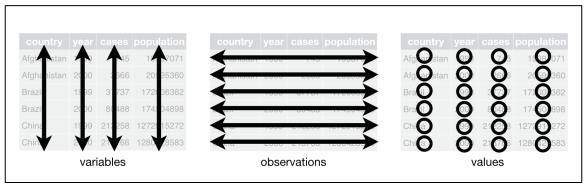
\includegraphics[width=0.7\linewidth]{./images/chp2/tidy} 

}

\caption{Visualisasi 3 rule tidy data (Sumber: Grolemund dan Wickham, 2017).}\label{fig:tidy}
\end{figure}

\hypertarget{input-data-pada-r-commander}{%
\section{\texorpdfstring{Input Data pada \texttt{R\ Commander}}{Input Data pada R Commander}}\label{input-data-pada-r-commander}}

Input data dapat dilakukan secara langsung pada \texttt{R\ Commander}. Input data secara langsung umumnya dilakukan jika jumlah data yag kita miliki relatif kecil. Untuk melakukanya jalakan tahapan berikut:

\begin{enumerate}
\def\labelenumi{\arabic{enumi}.}
\tightlist
\item
  Pada menu, klik \texttt{Data/New\ data\ set...}. Klik \texttt{OK},
\item
  Pada jedela yang muncul, ketikkan nama dataset yang kita inginkan. Klik \texttt{OK}
\item
  Pada jendela \texttt{Data\ Editor:Nama\_Dataset}, ketikkan data yang kita miliki.
\item
  Untuk menambah baris klik tombol \texttt{Add\ row}, sedangkan untuk menambah kolom klik tombol \texttt{Add\ column}.
\item
  Untuk mengubah nama kolom, klik pada bagian nama kolom dan ketikkan nama kolom yang diinginkan.
\item
  Secara \emph{default} \emph{rowname} akan dinamai urutan observasi. Namun, kita dapat memberikan nama pada masing-masing kolom dengan cara meng-klik nama baris pada tiap barisnya.
\item
  Untuk mengecek dataset yang telah kita buat, klik \emph{toolbar} \texttt{View\ data\ set}.
\end{enumerate}

Visualisasi tahapan tersebut ditampilkan pada Gambar \ref{fig:inputdata}.

\begin{figure}

{\centering 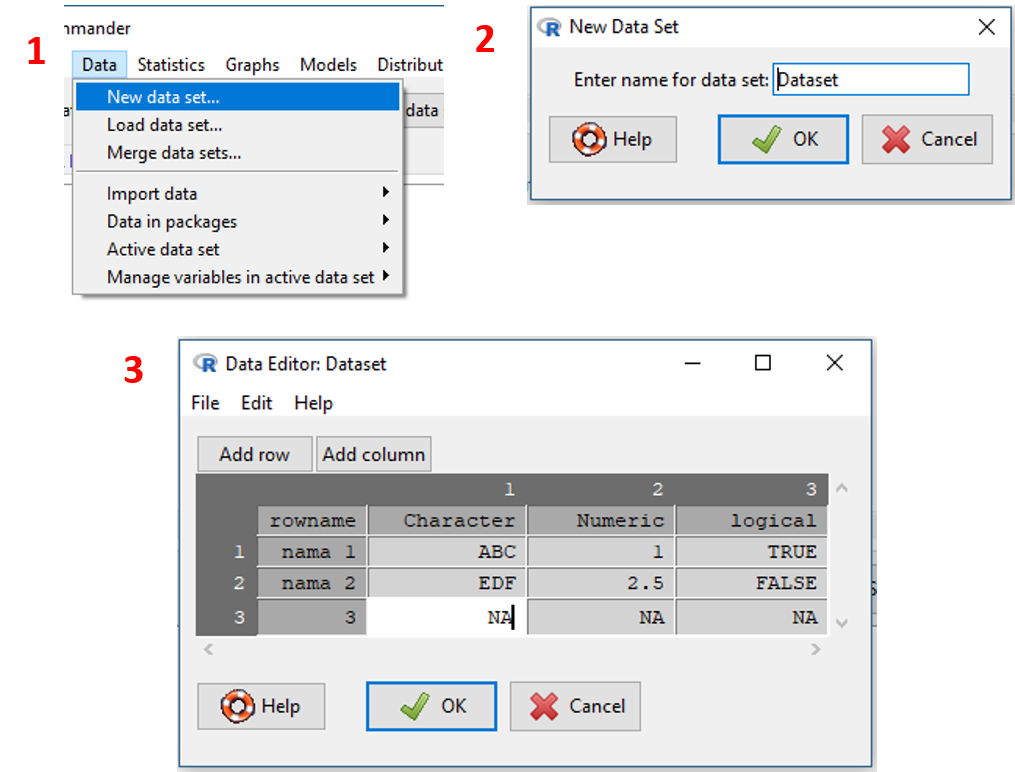
\includegraphics[width=0.7\linewidth]{./images/chp2/input_data} 

}

\caption{Visualisasi tahapan input dataset pada R Commander.}\label{fig:inputdata}
\end{figure}

Terdapat beberapa hal yang perlu diperhatikan pada proses input data, antara lain:

\begin{itemize}
\tightlist
\item
  Dalam pemberian \emph{rownames}. Jika \emph{rownames} mengandung spasi, input \emph{rownames} disertai tanda \emph{quote} (contoh:\texttt{"Nama\ Baris"}). Jika tidak ingin menggunakan spasi pada \emph{rownames}, gunakan tanda titik atau koma sebagai pemisah kata (contoh:\texttt{Nama.Baris} atau \texttt{Nama\_Baris}).
\item
  Pastikan \emph{rownames} bersifat unik (tidak ada duplikasi nama).
\item
  Pembaca dapat menggunakan tombol pada pada \emph{keyboard} untuk bernavigasi pada \emph{data editor} atau gunakan klik kiri pada sel yang ingin dituju.
\item
  Jenis data pada kolom akan secara otomatis ditentukan oleh seluruh data yang ada pada kolomnya. Jika data berupa angka, program secara otomatis mengkonversinya menjadi data \texttt{numeric}. Jika data berupa campuran angka atau karakter, secara otomatis program mengkonversinya menjadi \texttt{Character}.
\item
  Pembaca dapat memperluas area sel dengan cara menggeser sisi sel atau dengan cara memperluas melalui menggeser ujung jendela editor.
\item
  Dataset yang telah dibuat dapat diedit kembali dengan cara klik \emph{toolbar} \texttt{Edit\ data\ set}.
\end{itemize}

\hypertarget{impeks}{%
\section{Membaca Data dari File Eksternal}\label{impeks}}

Pada Chapter \ref{impeks}, pembaca akan mempelajari bagaimana cara melakukan import data dari berbagai sumber seperti \emph{plain text}, \emph{spreadsheets}, SPSS, STATA, SAS, dan Minitab. Sebelum melakukan hal tersebut terdapat beberapa hal yang perlu pembaca perhatikan, antara lain:

\begin{itemize}
\tightlist
\item
  Pastikan data berada dalam format \emph{tidy data} (lihat Chapter \ref{tidydata}), dan
\item
  Pastikan \emph{missing value} berada pada notasi yang konsisten.
\end{itemize}

Data yang berasal dari berbagai sumber akan memberikan format notasi \emph{missing value} yang berbeda-beda, misalnya data yag berasal dari database akan memberikan notasi \texttt{NULL} terhadap \emph{missing value}, sedangkan data yang berasal dari \emph{spreadsheet} akan memberikan notasi \emph{missing value} berdasarkan operasi yang dilakukan pada datanya (contoh: \texttt{\#VALUE!} untuk hasil operasi 2 buah objek berbeda tipe datanya). \texttt{RCommander} tidak dapat menangani kondisi di mana pada satu kolom data terdapat lebih dari 1 notasi \emph{missing value}. Untuk mengatasi hal tersebut, pembaca perlu menyeragamkan notasi \emph{missing value} pada data (contoh: mengubahnya menjadi notasi \texttt{NA} atau dikosongkan jika data bersumber dari \emph{spreadsheet}).

Pada Chapter \ref{impeks}, pembaca akan diberikan contoh bagaimana melakukan import data yang disajikan pada Tabel \ref{tab:mtcars}.

\begin{table}

\caption{\label{tab:mtcars}Sepuluh Observasi pertama dataset mtcars}
\centering
\begin{tabular}[t]{r|r|r|r|r|r|r|r|r|r|r}
\hline
mpg & cyl & disp & hp & drat & wt & qsec & vs & am & gear & carb\\
\hline
21.0 & 6 & 160.0 & 110 & 3.90 & 2.620 & 16.46 & 0 & 1 & 4 & 4\\
\hline
21.0 & 6 & 160.0 & 110 & 3.90 & 2.875 & 17.02 & 0 & 1 & 4 & 4\\
\hline
22.8 & 4 & 108.0 & 93 & 3.85 & 2.320 & 18.61 & 1 & 1 & 4 & 1\\
\hline
21.4 & 6 & 258.0 & 110 & 3.08 & 3.215 & 19.44 & 1 & 0 & 3 & 1\\
\hline
18.7 & 8 & 360.0 & 175 & 3.15 & 3.440 & 17.02 & 0 & 0 & 3 & 2\\
\hline
18.1 & 6 & 225.0 & 105 & 2.76 & 3.460 & 20.22 & 1 & 0 & 3 & 1\\
\hline
14.3 & 8 & 360.0 & 245 & 3.21 & 3.570 & 15.84 & 0 & 0 & 3 & 4\\
\hline
24.4 & 4 & 146.7 & 62 & 3.69 & 3.190 & 20.00 & 1 & 0 & 4 & 2\\
\hline
22.8 & 4 & 140.8 & 95 & 3.92 & 3.150 & 22.90 & 1 & 0 & 4 & 2\\
\hline
19.2 & 6 & 167.6 & 123 & 3.92 & 3.440 & 18.30 & 1 & 0 & 4 & 4\\
\hline
\end{tabular}
\end{table}

Adapun penjelasan terkait Tabel \ref{tab:mtcars} ditampilkan pada Tabel \ref{tab:mtcars2}

\begin{longtable}[]{@{}ll@{}}
\caption{\label{tab:mtcars2} Penjelasan variabel dataset mtcars.}\tabularnewline
\toprule
\textbf{Variabel} & \textbf{Keterangan}\tabularnewline
\midrule
\endfirsthead
\toprule
\textbf{Variabel} & \textbf{Keterangan}\tabularnewline
\midrule
\endhead
\texttt{mpg} & Mil/(US) galon\tabularnewline
\texttt{cyl} & Jumlah silinder\tabularnewline
\texttt{disp} & \emph{Displacement} (cu.in)\tabularnewline
\texttt{hp} & \emph{Gross horsepower}\tabularnewline
\texttt{drat} & Rasio gandar belakang\tabularnewline
\texttt{wt} & Berat (1000 lb)\tabularnewline
\texttt{qsec} & Watu tempuh 1/4 mil\tabularnewline
\texttt{vs} & Mesin (0=\emph{V-shape}, 1=\emph{straight})\tabularnewline
\texttt{am} & Transmisi (0=otomatis, 1=manual)\tabularnewline
\texttt{gear} & Jumlah \emph{gear} depan\tabularnewline
\texttt{carb} & Jumlah karburator\tabularnewline
\bottomrule
\end{longtable}

\hypertarget{membaca-data-dari-sumber-plain-text}{%
\subsection{\texorpdfstring{Membaca Data dari Sumber \emph{Plain Text}}{Membaca Data dari Sumber Plain Text}}\label{membaca-data-dari-sumber-plain-text}}

Terdapat 3 buah metode untuk membaca data dari \emph{plain text}. Metode tersebut dibagi berdasarkan lokasi file \emph{plain text} tersebut berada.

\textbf{Membaca file yang berada pada sistem lokal}

\begin{enumerate}
\def\labelenumi{\arabic{enumi}.}
\tightlist
\item
  Pada menu \texttt{Data}, klik \texttt{Data/Import\ data/from\ text\ file,clipboard,or\ URL...}.
\item
  Pada jendela yang muncul, isikan spesifikasi file (lihat Tabel \ref{tab:readpltext}) dan nama objek dataset yang diinginkan. Pada bagian \texttt{Location\ of\ Data\ File} pilih \texttt{Local\ file\ system}. Klik \texttt{OK}.
\item
  Pada jendela \texttt{Windows\ Explorer} yang muncul, pilih file yang hendak dibaca. Klik \texttt{Open}.
\item
  Untuk melihat dataset yang berhasil dibuat, klik pada \emph{toolbar} \texttt{View\ data\ set}.
\end{enumerate}

Visualisasi tahapan tersebut ditampilkan pada Gambar \ref{fig:implocal}.

\begin{figure}

{\centering 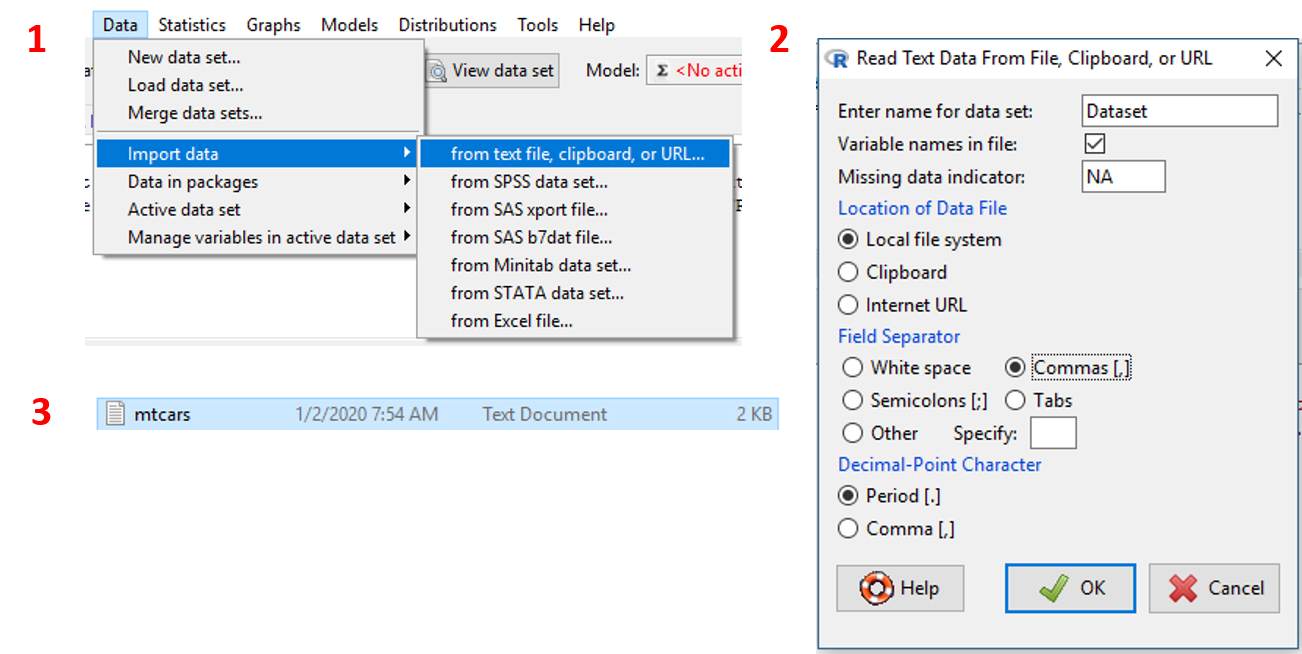
\includegraphics[width=0.7\linewidth]{./images/chp2/implocal} 

}

\caption{Visualisasi tahapan membaca file plain text dari sistem lokal.}\label{fig:implocal}
\end{figure}

\textbf{Membaca file yang berada pada \emph{clipboard}}

\begin{enumerate}
\def\labelenumi{\arabic{enumi}.}
\tightlist
\item
  \emph{Higlight} tabel dataset yang pembaca miliki dan \emph{copy} dataset tersebut. Dataset tersebut selanjutnya akan tersimpan pada \emph{clipboard}.
\item
  Pada menu \texttt{Data}, klik \texttt{Data/Import\ data/from\ text\ file,clipboard,or\ URL...}.
\item
  Pada jendela yang muncul, isikan spesifikasi file (lihat Tabel \ref{tab:readpltext}) dan nama objek dataset yang diinginkan. Pada bagian \texttt{Location\ of\ Data\ File} pilih \texttt{clipboard} .Klik \texttt{OK}.
\item
  Dataset akan secara otomatis dibuat oleh program dengan mengambil data yang tersimpan pada \emph{clipboard}.
\item
  Untuk melihat dataset yang berhasil dibuat, klik pada \emph{toolbar} \texttt{View\ data\ set}.
\end{enumerate}

\textbf{Membaca file yang berada pada URL}

\begin{enumerate}
\def\labelenumi{\arabic{enumi}.}
\tightlist
\item
  \emph{Copy} halaman URL lokasi dataset berada.
\item
  Pada menu \texttt{Data}, klik \texttt{Data/Import\ data/from\ text\ file,clipboard,or\ URL...}.
\item
  Pada jendela yang muncul, isikan spesifikasi file (lihat Tabel \ref{tab:readpltext}) dan nama objek dataset yang diinginkan. Pada bagian \texttt{Location\ of\ Data\ File} pilih \texttt{Internet\ URL}. Klik \texttt{OK}.
\item
  Pada jendela yang muncul tempelkan (\emph{pasting}) halaman URL yang telah di \emph{copy} sebelumnya.
\item
  Untuk melihat dataset yang berhasil dibuat, klik pada \emph{toolbar} \texttt{View\ data\ set}.
\end{enumerate}

Visualisasi tahapan tersebut ditampilkan pada Gambar \ref{fig:impurl}.

\begin{figure}

{\centering 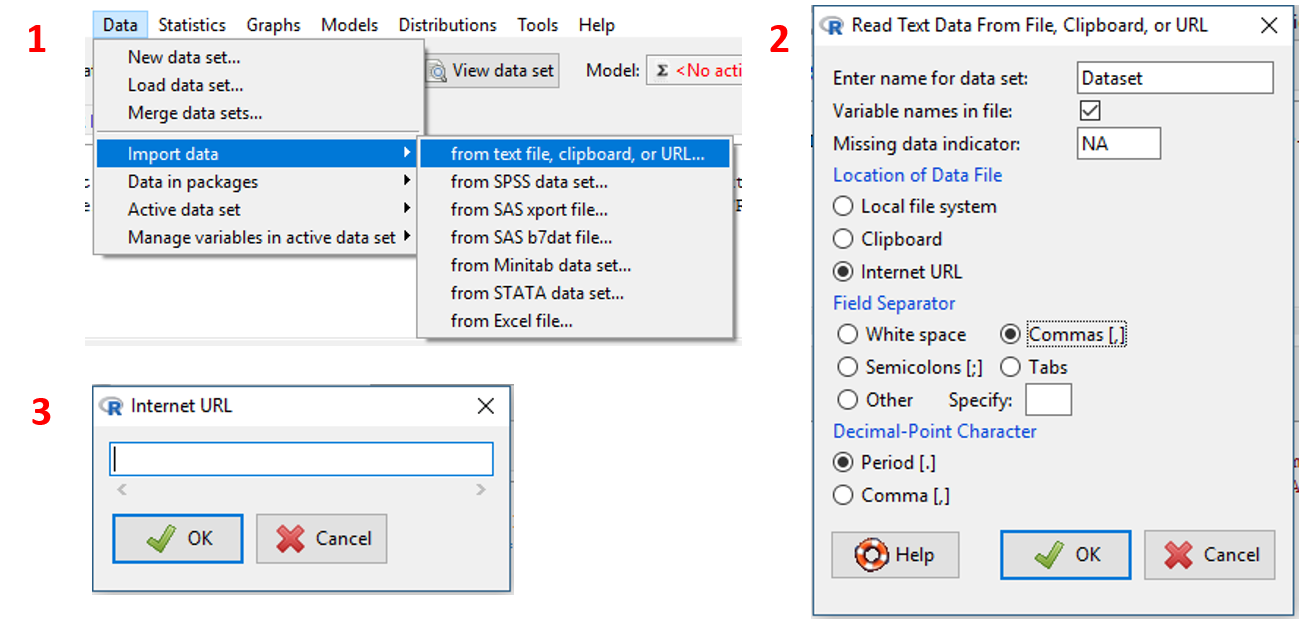
\includegraphics[width=0.7\linewidth]{./images/chp2/impurl} 

}

\caption{Visualisasi tahapan membaca file plain text dari internet URL.}\label{fig:impurl}
\end{figure}

Sintaks yang muncul pada \texttt{R\ Console} saat proses telah dilakukan adalah sebagai berikut:

\begin{Shaded}
\begin{Highlighting}[]
\CommentTok{# sistem lokal}
\NormalTok{Dataset <-}\StringTok{ }\KeywordTok{read.table}\NormalTok{(}\StringTok{"D:/mtcars.txt"}\NormalTok{, }\DataTypeTok{header=}\OtherTok{TRUE}\NormalTok{, }
                      \DataTypeTok{sep=}\StringTok{""}\NormalTok{, }\DataTypeTok{na.strings=}\StringTok{"NA"}\NormalTok{, }\DataTypeTok{dec=}\StringTok{"."}\NormalTok{,}
                      \DataTypeTok{strip.white=}\OtherTok{TRUE}\NormalTok{)}
\CommentTok{# clipboard}
\NormalTok{Dataset <-}\StringTok{ }\KeywordTok{read.table}\NormalTok{(}\StringTok{"clipboard"}\NormalTok{, }\DataTypeTok{header=}\OtherTok{TRUE}\NormalTok{, }
                      \DataTypeTok{sep=}\StringTok{""}\NormalTok{, }\DataTypeTok{na.strings=}\StringTok{"NA"}\NormalTok{,}
                      \DataTypeTok{dec=}\StringTok{"."}\NormalTok{, }\DataTypeTok{strip.white=}\OtherTok{TRUE}\NormalTok{)}
\CommentTok{# URL}
\NormalTok{Dataset <-}\StringTok{ }\KeywordTok{read.table}\NormalTok{(}\StringTok{"www.abcde.com/mtcars.txt"}\NormalTok{, }
                      \DataTypeTok{header=}\OtherTok{TRUE}\NormalTok{, }\DataTypeTok{sep=}\StringTok{""}\NormalTok{,}\DataTypeTok{na.strings=}\StringTok{"NA"}\NormalTok{, }
                      \DataTypeTok{dec=}\StringTok{"."}\NormalTok{, }\DataTypeTok{strip.white=}\OtherTok{TRUE}\NormalTok{)}
\end{Highlighting}
\end{Shaded}

\begin{longtable}[]{@{}llll@{}}
\caption{\label{tab:readpltext} Penjelasan terkait item pada jendela Read Text Data From File, Clipboard, or URL.}\tabularnewline
\toprule
\begin{minipage}[b]{0.04\columnwidth}\raggedright
\textbf{No.}\strut
\end{minipage} & \begin{minipage}[b]{0.17\columnwidth}\raggedright
\textbf{Item}\strut
\end{minipage} & \begin{minipage}[b]{0.10\columnwidth}\raggedright
\textbf{Jenis Input}\strut
\end{minipage} & \begin{minipage}[b]{0.58\columnwidth}\raggedright
\textbf{Keterangan}\strut
\end{minipage}\tabularnewline
\midrule
\endfirsthead
\toprule
\begin{minipage}[b]{0.04\columnwidth}\raggedright
\textbf{No.}\strut
\end{minipage} & \begin{minipage}[b]{0.17\columnwidth}\raggedright
\textbf{Item}\strut
\end{minipage} & \begin{minipage}[b]{0.10\columnwidth}\raggedright
\textbf{Jenis Input}\strut
\end{minipage} & \begin{minipage}[b]{0.58\columnwidth}\raggedright
\textbf{Keterangan}\strut
\end{minipage}\tabularnewline
\midrule
\endhead
\begin{minipage}[t]{0.04\columnwidth}\raggedright
1.\strut
\end{minipage} & \begin{minipage}[t]{0.17\columnwidth}\raggedright
\texttt{Enter\ name\ for\ data\ set}\strut
\end{minipage} & \begin{minipage}[t]{0.10\columnwidth}\raggedright
\emph{text input}\strut
\end{minipage} & \begin{minipage}[t]{0.58\columnwidth}\raggedright
Input nama dataset yang diinginkan sebagai output\strut
\end{minipage}\tabularnewline
\begin{minipage}[t]{0.04\columnwidth}\raggedright
2.\strut
\end{minipage} & \begin{minipage}[t]{0.17\columnwidth}\raggedright
\texttt{Variable\ name\ in\ file}\strut
\end{minipage} & \begin{minipage}[t]{0.10\columnwidth}\raggedright
\emph{Check box}\strut
\end{minipage} & \begin{minipage}[t]{0.58\columnwidth}\raggedright
Jika di centang, program membaca baris pertama tabel sebagai nama kolom\strut
\end{minipage}\tabularnewline
\begin{minipage}[t]{0.04\columnwidth}\raggedright
3.\strut
\end{minipage} & \begin{minipage}[t]{0.17\columnwidth}\raggedright
\texttt{Missing\ value\ indikator}\strut
\end{minipage} & \begin{minipage}[t]{0.10\columnwidth}\raggedright
\emph{text input}\strut
\end{minipage} & \begin{minipage}[t]{0.58\columnwidth}\raggedright
Karakter yang mengidikasikan missing value dalam file (misal: \emph{White space}, NA, NaN, dll)\strut
\end{minipage}\tabularnewline
\begin{minipage}[t]{0.04\columnwidth}\raggedright
4.\strut
\end{minipage} & \begin{minipage}[t]{0.17\columnwidth}\raggedright
\texttt{Location\ of\ Data\ File}\strut
\end{minipage} & \begin{minipage}[t]{0.10\columnwidth}\raggedright
\emph{radio button}\strut
\end{minipage} & \begin{minipage}[t]{0.58\columnwidth}\raggedright
Lokasi file yang akan dibaca berada\strut
\end{minipage}\tabularnewline
\begin{minipage}[t]{0.04\columnwidth}\raggedright
5.\strut
\end{minipage} & \begin{minipage}[t]{0.17\columnwidth}\raggedright
\texttt{Field\ Separator}\strut
\end{minipage} & \begin{minipage}[t]{0.10\columnwidth}\raggedright
\emph{radio button}\strut
\end{minipage} & \begin{minipage}[t]{0.58\columnwidth}\raggedright
Pemisah antar kolom data yang digunakan\strut
\end{minipage}\tabularnewline
\begin{minipage}[t]{0.04\columnwidth}\raggedright
6.\strut
\end{minipage} & \begin{minipage}[t]{0.17\columnwidth}\raggedright
\texttt{Decimal-Point\ Character}\strut
\end{minipage} & \begin{minipage}[t]{0.10\columnwidth}\raggedright
\emph{radio button}\strut
\end{minipage} & \begin{minipage}[t]{0.58\columnwidth}\raggedright
Karakter yang digunakan sebagai penunjuk \emph{decimal-point}\strut
\end{minipage}\tabularnewline
\bottomrule
\end{longtable}

\hypertarget{membaca-data-dari-sumber-spreadsheet-dan-lainnya}{%
\subsection{\texorpdfstring{Membaca Data dari Sumber \emph{Spreadsheet} dan Lainnya}{Membaca Data dari Sumber Spreadsheet dan Lainnya}}\label{membaca-data-dari-sumber-spreadsheet-dan-lainnya}}

Format data lain yang dapat dibaca oleg \texttt{R\ Commander} adalah \texttt{xlsx} (Excel) ,\texttt{.dta} (STATA), \texttt{.sav} (SPSS), \texttt{.sas7bdat} dan \texttt{.xport} (SAS), serta \texttt{.mtp} (minitab). Cara membaca data dengan format tersebut cukup sederhana dilakukan pada \texttt{R\ Commander}. Pembaca hanya perlu menuju menu \texttt{Data/Import\ data} dan memilih sumber data yang ingin dibaca. Pada jendela yang muncul (kecuali format \texttt{.xport}) pembaca diminta untuk melakukan sejumlah konfigurasi seperti apakah \emph{rownames} terletak pada kolom pertama, apakah perlu mengubah jenis data karakter menjadi faktor, dll. Pada kondisi dimana pembaca diminta untuk mengkonversi karakter menjadi faktor, penulis menyarankan untuk tidak melakukannya saat awal membaca data sebab akan menyulitkan pada saat melakukan analisis data selanjutnya. Konversi karakter menjadi faktor dilakukan pada sejumlah variabel yang memang ingin diubah menjadi faktor (bisa numerik atau karakter). Tampilan jendela konfigurasi awal saat membaca data ditampilkan pada Gambar \ref{fig:impanother}.

\begin{figure}

{\centering 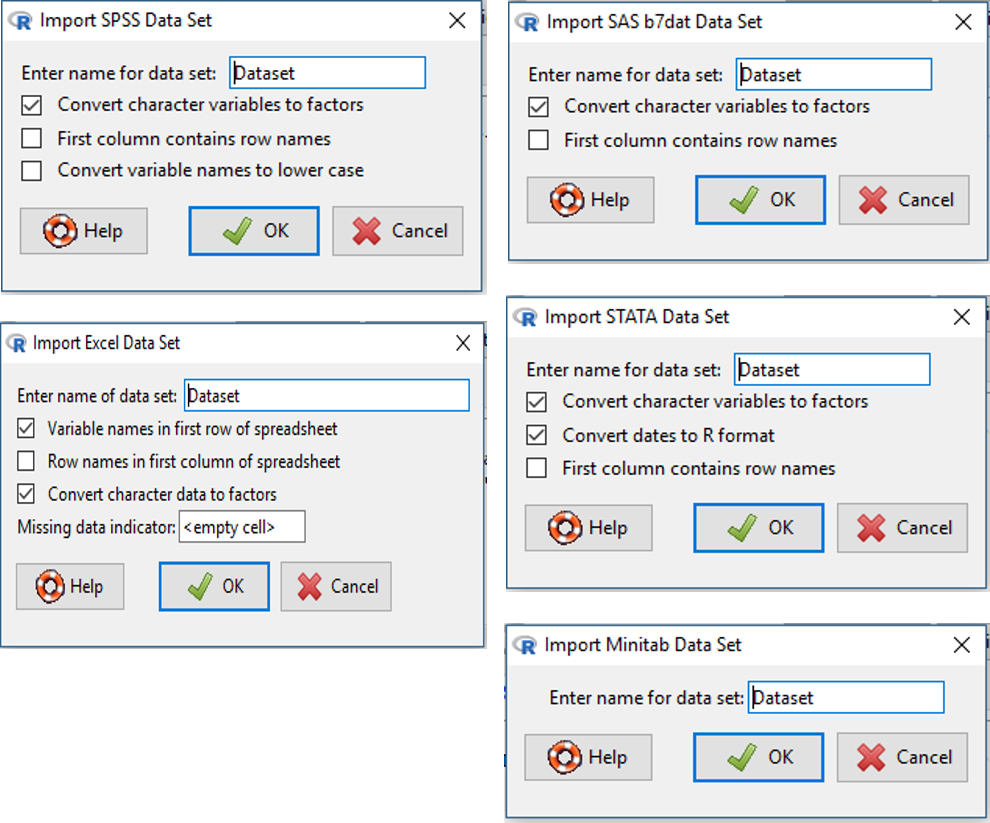
\includegraphics[width=0.7\linewidth]{./images/chp2/impanother} 

}

\caption{Tampilan jendela konfigurasi import data berbagai format file.}\label{fig:impanother}
\end{figure}

Contoh sintaks yang akan muncul saat proses tersebut selesai adalah sebagai berikut:

\begin{Shaded}
\begin{Highlighting}[]
\CommentTok{# .xlsx}
\NormalTok{Dataset <-}\StringTok{ }\KeywordTok{readXL}\NormalTok{(}\StringTok{"D:/mtcars.xlsx"}\NormalTok{, }\DataTypeTok{rownames=}\OtherTok{FALSE}\NormalTok{, }
                  \DataTypeTok{header=}\OtherTok{TRUE}\NormalTok{, }\DataTypeTok{na=}\StringTok{""}\NormalTok{, }\DataTypeTok{sheet=}\StringTok{"mtcars"}\NormalTok{,}
                  \DataTypeTok{stringsAsFactors=}\OtherTok{TRUE}\NormalTok{)}

\CommentTok{# .sav}
\NormalTok{Dataset <-}\StringTok{ }\KeywordTok{readSPSS}\NormalTok{(}\StringTok{"D:/mtcars.sav"}\NormalTok{, }\DataTypeTok{rownames=}\OtherTok{FALSE}\NormalTok{,}
                    \DataTypeTok{stringsAsFactors=}\OtherTok{TRUE}\NormalTok{, }\DataTypeTok{tolower=}\OtherTok{FALSE}\NormalTok{)}

\CommentTok{# .xport}
\NormalTok{Datasets <-}\StringTok{ }\KeywordTok{read.xport}\NormalTok{(}\StringTok{"D:/mtcars.xport"}\NormalTok{)}

\CommentTok{# .sasb7dat}
\NormalTok{Dataset <-}\StringTok{ }\KeywordTok{readSAS}\NormalTok{(}\StringTok{"D:/mtcars.sas7bdat"}\NormalTok{,}
                   \DataTypeTok{stringsAsFactors=}\OtherTok{TRUE}\NormalTok{, }\DataTypeTok{rownames=}\OtherTok{FALSE}\NormalTok{)}

\CommentTok{# .dta}
\NormalTok{Dataset <-}\StringTok{ }\KeywordTok{readStata}\NormalTok{(}\StringTok{"D:/mtcars.dta"}\NormalTok{, }\DataTypeTok{convert.dates=}\OtherTok{TRUE}\NormalTok{,}
                     \DataTypeTok{stringsAsFactors=}\OtherTok{TRUE}\NormalTok{, }\DataTypeTok{rownames=}\OtherTok{FALSE}\NormalTok{)}
\end{Highlighting}
\end{Shaded}

\hypertarget{membaca-data-dari-paket}{%
\section{Membaca Data dari Paket}\label{membaca-data-dari-paket}}

\hypertarget{memuat-paket}{%
\subsection{Memuat Paket}\label{memuat-paket}}

Jika pembaca ingin mengakses dataset dari paket yang pembaca inginkan, pembaca dapat menjalankan perintah berikut pada \texttt{R\ Console}:

\begin{Shaded}
\begin{Highlighting}[]
\KeywordTok{library}\NormalTok{(nama_paket)}
\end{Highlighting}
\end{Shaded}

Jika paket tersebut belum terpasang, jalankan perintah berikut:

\begin{Shaded}
\begin{Highlighting}[]
\KeywordTok{install.packages}\NormalTok{(}\StringTok{"nama_paket"}\NormalTok{)}
\end{Highlighting}
\end{Shaded}

Jika pembaca kesulitan menggunakan cara tersebut, pembaca dapat menggunakan metode yang sama dengan cara memasang paket \texttt{Rcmdr} (lihat Chapter \ref{installrcmdr}) dan memuat paket \texttt{Rcmdr} (lihat Chapter \ref{loadrcmdr}).

\hypertarget{memuat-dataset-pada-paket}{%
\subsection{Memuat Dataset Pada Paket}\label{memuat-dataset-pada-paket}}

Untuk mengecek dataset apa saja yang tersedia paket yang telah aktif, lakukan langkah-langkah berikut:

\begin{enumerate}
\def\labelenumi{\arabic{enumi}.}
\tightlist
\item
  Pada menu \texttt{Data}, klik \texttt{Data/Data\ in\ packages/List\ data\ set\ in\ packages}.
\item
  Jendela \texttt{R\ data\ sets} yang memberikan daftar seluruh dataset yang tersedia pada paket yang telah dimuat akan muncul.
\end{enumerate}

Pada proses tersebut, \texttt{R\ Script} akan memunculkan sebuah sintaks berikut:

\begin{Shaded}
\begin{Highlighting}[]
\KeywordTok{data}\NormalTok{()}
\end{Highlighting}
\end{Shaded}

Visualisasi tahapan tersebut ditampilkan pada Gambar \ref{fig:loaddata}.

\begin{figure}

{\centering 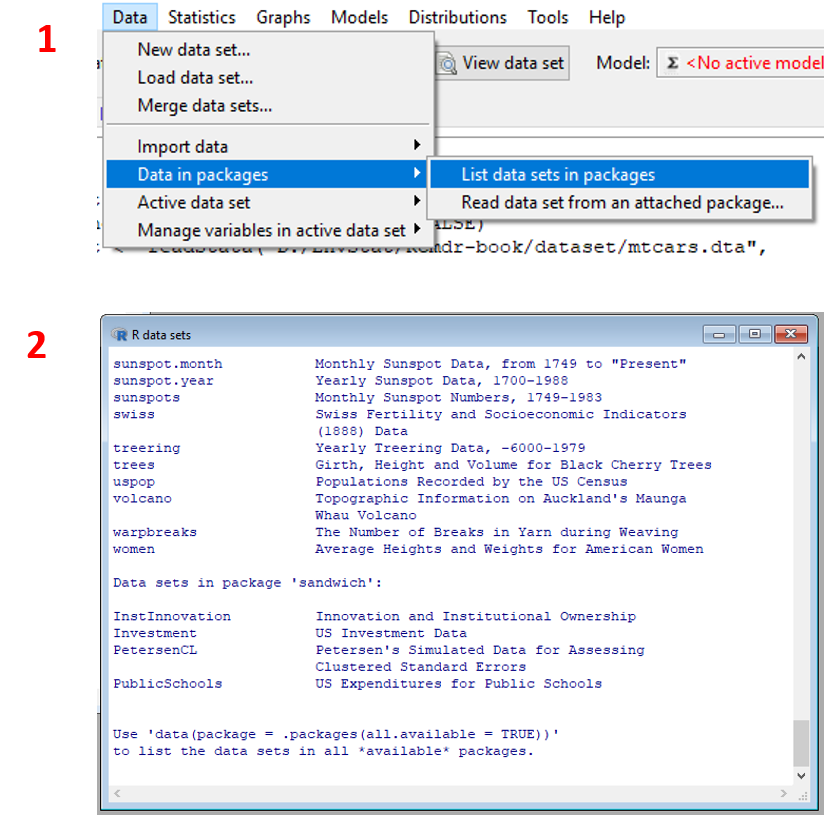
\includegraphics[width=0.7\linewidth]{./images/chp2/loaddata} 

}

\caption{Tampilan langkah menampilkan seluruh dataset dari paket.}\label{fig:loaddata}
\end{figure}

\hypertarget{membaca-data}{%
\subsection{Membaca Data}\label{membaca-data}}

Untuk membaca dataset dari paket, jalankan langkah-langkah berikut:

\begin{enumerate}
\def\labelenumi{\arabic{enumi}.}
\tightlist
\item
  Pada menu \texttt{Data}, klik \texttt{Data/Data\ in\ packages/Read\ data\ set\ from\ an\ attached\ package...}.
\item
  Pada kotak \texttt{package}, \emph{double click} paket yang pembaca ingin lihat datasetnya. Daftar dataset selanjutnya akan muncul pada kotak \texttt{Data\ set}.
\item
  Pilih dataset yang pembaca ingin baca. Pembaca dapat merubah nama dataset yang akan dibaca melalui kotak \texttt{Enter\ nama\ of\ data\ set}. Klik \texttt{OK}.
\item
  Untuk melihat dataset yang telah dimuat, klik \emph{toolbar} \texttt{View\ data\ set}.
\end{enumerate}

Pada contoh berikut, penulis mencoba memuat dataset \texttt{mtcars} dari paket \texttt{datasets}. Sintaks yang muncul pada \texttt{R\ Script} dan kotat \texttt{Output} adalah sebagai berikut:

\begin{Shaded}
\begin{Highlighting}[]
\KeywordTok{data}\NormalTok{(mtcars, }\DataTypeTok{package=}\StringTok{"datasets"}\NormalTok{)}
\end{Highlighting}
\end{Shaded}

Visualisasi tahapan tersebut ditampilkan pada Gambar \ref{fig:datapaket}.

\begin{figure}

{\centering 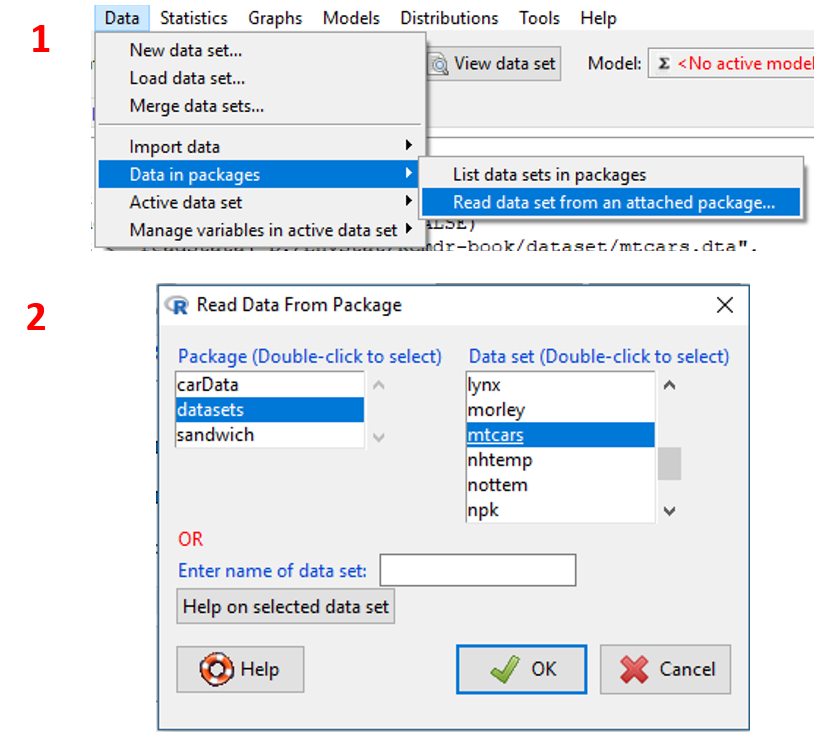
\includegraphics[width=0.7\linewidth]{./images/chp2/datapaket} 

}

\caption{Tampilan langkah membaca dataset pada paket.}\label{fig:datapaket}
\end{figure}

\hypertarget{meyimpan-dan-memuat-data}{%
\section{Meyimpan dan Memuat Data}\label{meyimpan-dan-memuat-data}}

\hypertarget{menyimpan-dataset}{%
\subsection{Menyimpan Dataset}\label{menyimpan-dataset}}

Data pada \texttt{R\ Commander} dapat disimpan ke dalam format \texttt{.RData}. Penyimpanan dalam format tersebut akan mempermudah pembaca untuk memperoleh data tersebut saat akan dibaca kembali dan pembaca tidak perlu mengulangi kembali proses membaca data pada bagian sebelumnya.
Untuk dapat menyimpan data menggunakan format \texttt{.RData} yang telah berhasil dibaca pada \texttt{R\ Commander}, pembaca dapat melakukan langkah-langkah berikut:

\begin{enumerate}
\def\labelenumi{\arabic{enumi}.}
\tightlist
\item
  Pada menu \texttt{Data}, klik \texttt{Data/Active\ data\ set/Save\ active\ data\ set...}.
\item
  Pada jendela \texttt{Windows\ Explorer} yang muncul, navigasikan ke lokasi atau folder di mana data tersebut akan disimpan. Beri nama data tersebut sesuai dengan nama yang diinginkan. Klik \texttt{Save}.
\end{enumerate}

Visualisasi tahapan tersebut ditampilkan pada Gambar \ref{fig:saverdata}.

\begin{figure}

{\centering 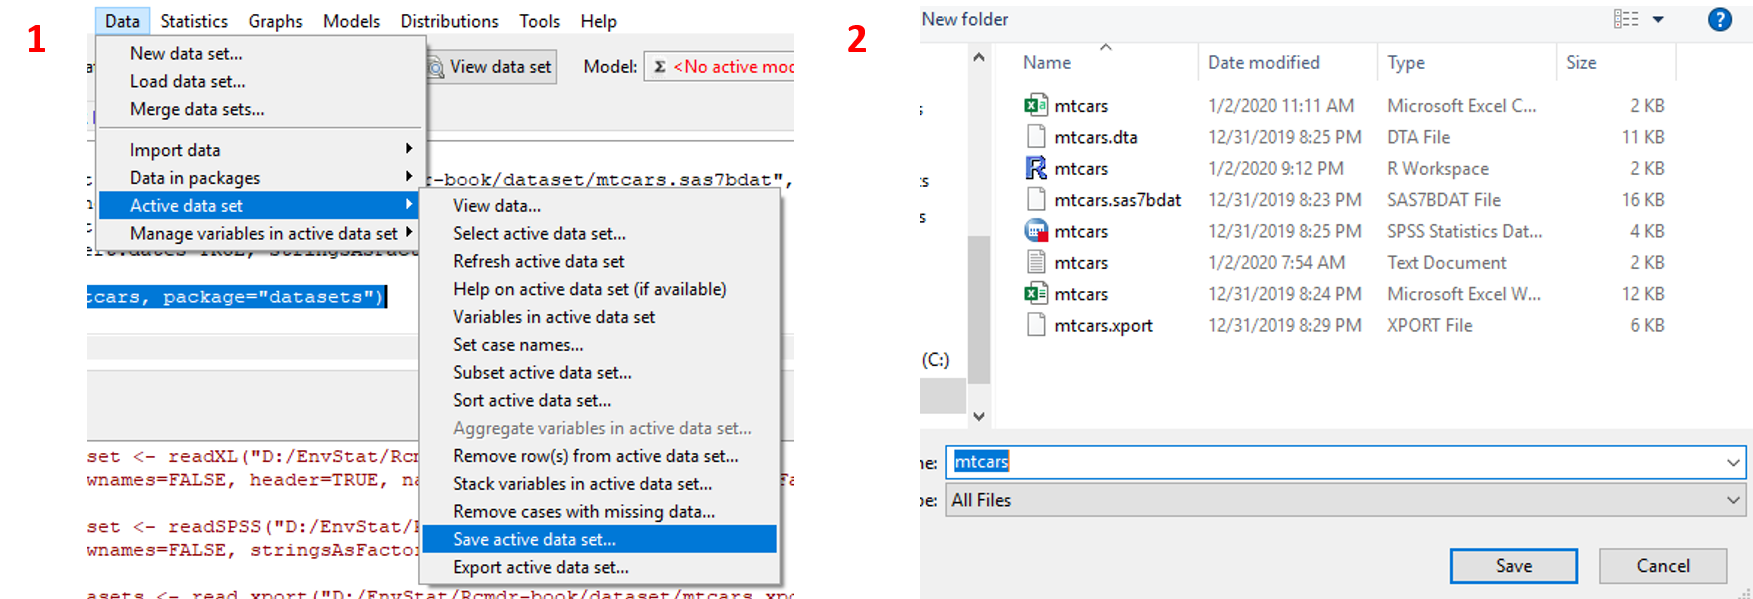
\includegraphics[width=0.7\linewidth]{./images/chp2/saverdata} 

}

\caption{Tampilan tahapan menyimpan data ke dalam format RData.}\label{fig:saverdata}
\end{figure}

Pada \texttt{R\ Script} dan kotak \texttt{Output} akan muncul sintaks berikut yang menandakan bahwa data yang ada pada \texttt{R\ Commander} telah disimpan pada folder yang telah penulis inginkan.

\begin{Shaded}
\begin{Highlighting}[]
\KeywordTok{save}\NormalTok{(}\StringTok{"mtcars"}\NormalTok{, }\DataTypeTok{file=}\StringTok{"D:/EnvStat/Rcmdr-book/dataset/mtcars.RData"}\NormalTok{)}
\end{Highlighting}
\end{Shaded}

Selain menyimpan data ke dalam format \texttt{.RData}, \texttt{R\ Commander} juga dapat menyimpan data ke dalam format \texttt{.csv}. Untuk melakukannya jalankan langkah berikut:

\begin{enumerate}
\def\labelenumi{\arabic{enumi}.}
\tightlist
\item
  Pada menu \texttt{Data}, klik \texttt{Data/Active\ data\ set/Export\ active\ data\ set...}.
\item
  Pada jendela yang muncul, spesifikasikan format data yang akan disimpan (lihat Tabel \ref{tab:exdata}).
\item
  Pada jendela \texttt{Windows\ Explorer} yang muncul, navigasikan ke lokasi atau folder di mana data tersebut akan disimpan. Beri nama data tersebut sesuai dengan nama yang diinginkan. Klik \texttt{Save}.
\end{enumerate}

Visualisasi tahapan tersebut ditampilkan pada Gambar \ref{fig:savecsv}.

\begin{figure}

{\centering 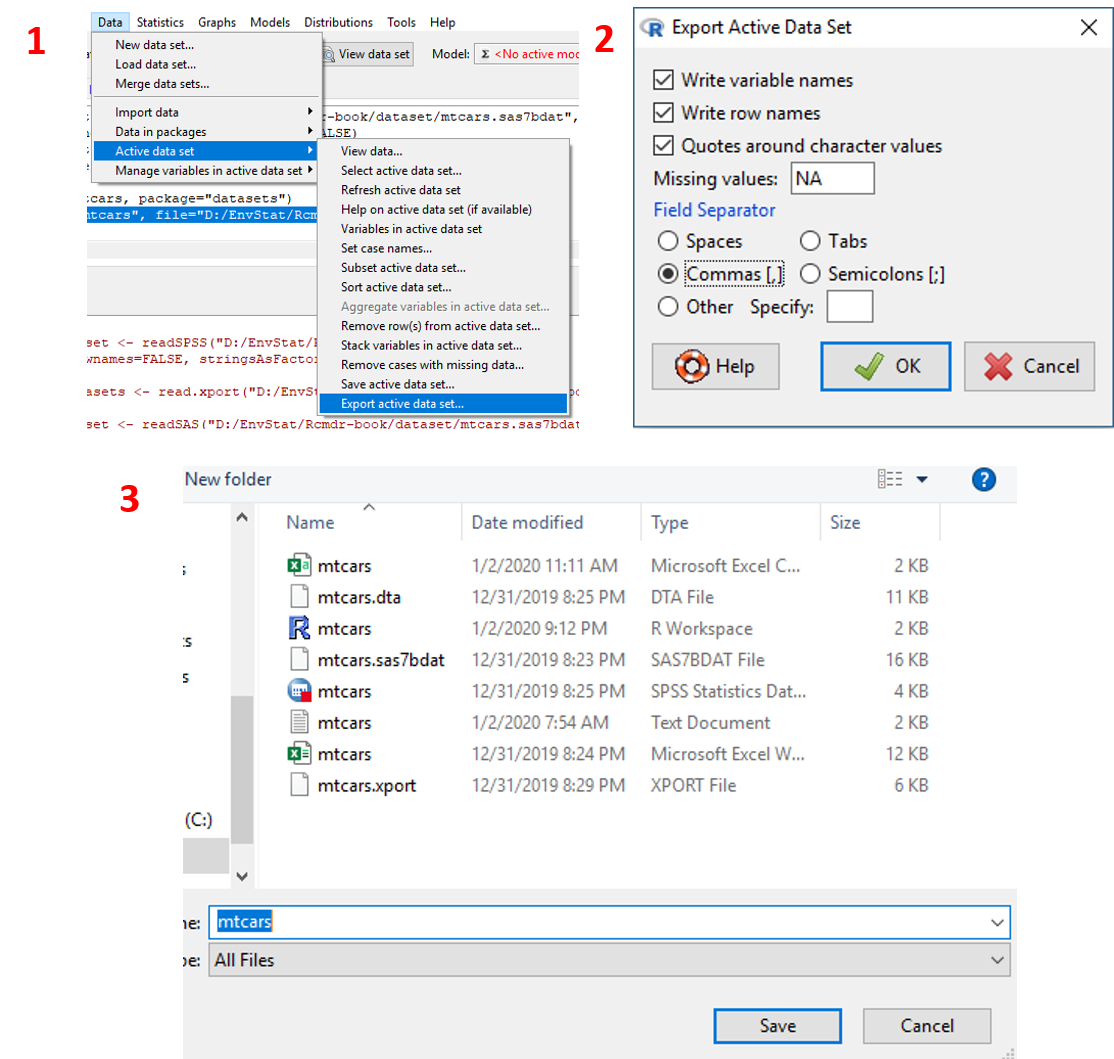
\includegraphics[width=0.7\linewidth]{./images/chp2/savecsv} 

}

\caption{Tampilan tahapan menyimpan data ke dalam format csv.}\label{fig:savecsv}
\end{figure}

Pada \texttt{R\ Script} dan kotak \texttt{Output} akan muncul sintaks berikut yang menandakan bahwa data yang ada pada \texttt{R\ Commander} telah disimpan pada folder yang telah penulis inginkan.

\begin{Shaded}
\begin{Highlighting}[]
\KeywordTok{write.table}\NormalTok{(mtcars, }\StringTok{"D:/mtcars2.csv"}\NormalTok{, }\DataTypeTok{sep=}\StringTok{","}\NormalTok{, }
            \DataTypeTok{col.names=}\OtherTok{TRUE}\NormalTok{, }\DataTypeTok{row.names=}\OtherTok{TRUE}\NormalTok{, }
            \DataTypeTok{quote=}\OtherTok{TRUE}\NormalTok{, }\DataTypeTok{na=}\StringTok{"NA"}\NormalTok{)}
\end{Highlighting}
\end{Shaded}

\begin{longtable}[]{@{}llll@{}}
\caption{\label{tab:exdata} Penjelasan item jendela Export active data set.}\tabularnewline
\toprule
\begin{minipage}[b]{0.05\columnwidth}\raggedright
\textbf{No.}\strut
\end{minipage} & \begin{minipage}[b]{0.23\columnwidth}\raggedright
\textbf{Item}\strut
\end{minipage} & \begin{minipage}[b]{0.10\columnwidth}\raggedright
\textbf{Jenis Imput}\strut
\end{minipage} & \begin{minipage}[b]{0.51\columnwidth}\raggedright
\textbf{Keterangan}\strut
\end{minipage}\tabularnewline
\midrule
\endfirsthead
\toprule
\begin{minipage}[b]{0.05\columnwidth}\raggedright
\textbf{No.}\strut
\end{minipage} & \begin{minipage}[b]{0.23\columnwidth}\raggedright
\textbf{Item}\strut
\end{minipage} & \begin{minipage}[b]{0.10\columnwidth}\raggedright
\textbf{Jenis Imput}\strut
\end{minipage} & \begin{minipage}[b]{0.51\columnwidth}\raggedright
\textbf{Keterangan}\strut
\end{minipage}\tabularnewline
\midrule
\endhead
\begin{minipage}[t]{0.05\columnwidth}\raggedright
1.\strut
\end{minipage} & \begin{minipage}[t]{0.23\columnwidth}\raggedright
\texttt{Write\ variable\ names}\strut
\end{minipage} & \begin{minipage}[t]{0.10\columnwidth}\raggedright
\emph{check box}\strut
\end{minipage} & \begin{minipage}[t]{0.51\columnwidth}\raggedright
pilihan apakah nama variabel akan disertakan ke dalam file csv\strut
\end{minipage}\tabularnewline
\begin{minipage}[t]{0.05\columnwidth}\raggedright
2.\strut
\end{minipage} & \begin{minipage}[t]{0.23\columnwidth}\raggedright
\texttt{Write\ row\ names}\strut
\end{minipage} & \begin{minipage}[t]{0.10\columnwidth}\raggedright
\emph{check box}\strut
\end{minipage} & \begin{minipage}[t]{0.51\columnwidth}\raggedright
pilihan apakah nama baris disertakan ke dalam file csv\strut
\end{minipage}\tabularnewline
\begin{minipage}[t]{0.05\columnwidth}\raggedright
3.\strut
\end{minipage} & \begin{minipage}[t]{0.23\columnwidth}\raggedright
\texttt{Quotes\ around\ character\ values}\strut
\end{minipage} & \begin{minipage}[t]{0.10\columnwidth}\raggedright
\emph{check box}\strut
\end{minipage} & \begin{minipage}[t]{0.51\columnwidth}\raggedright
pilihan apakah tipe data karakter diberi tanda petik\strut
\end{minipage}\tabularnewline
\begin{minipage}[t]{0.05\columnwidth}\raggedright
4.\strut
\end{minipage} & \begin{minipage}[t]{0.23\columnwidth}\raggedright
\texttt{Missing\ values}\strut
\end{minipage} & \begin{minipage}[t]{0.10\columnwidth}\raggedright
\emph{text input}\strut
\end{minipage} & \begin{minipage}[t]{0.51\columnwidth}\raggedright
simbol atau karakter \emph{missing value} yang digunakan pada file csv\strut
\end{minipage}\tabularnewline
\begin{minipage}[t]{0.05\columnwidth}\raggedright
5.\strut
\end{minipage} & \begin{minipage}[t]{0.23\columnwidth}\raggedright
\texttt{Field\ Separator}\strut
\end{minipage} & \begin{minipage}[t]{0.10\columnwidth}\raggedright
\emph{radio button}\strut
\end{minipage} & \begin{minipage}[t]{0.51\columnwidth}\raggedright
pemisah antar kolom data yang digunakan\strut
\end{minipage}\tabularnewline
\bottomrule
\end{longtable}

\hypertarget{memuat-data}{%
\subsection{Memuat Data}\label{memuat-data}}

Data yang telah disimpan ke dalam format \texttt{.RData} dapat langsung dimuat ke dalam \texttt{R\ Commander} tanpa perlu menspesifikasikan kembali format data yang hendak dibaca. Untuk melakukannya jalankan langkah berikut:

\begin{enumerate}
\def\labelenumi{\arabic{enumi}.}
\tightlist
\item
  Pada menu \texttt{Data}, klik \texttt{Data/Load\ data\ set...}.
\item
  Pada jendela \texttt{Windows\ Explorer} yang muncul, navigasikan ke lokasi atau folder di mana data tersebut berada. Pilih data yang akan dimuat. Klik \texttt{Open}.
\end{enumerate}

Visualisasi tahapan tersebut ditampilkan pada Gambar \ref{fig:loadrdata}.

\begin{figure}

{\centering 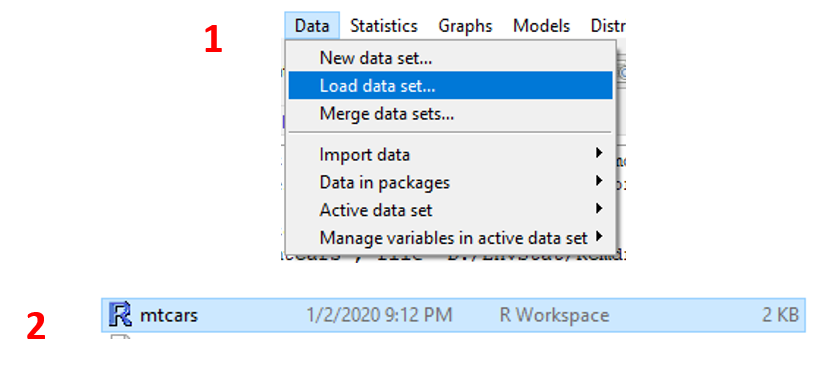
\includegraphics[width=0.7\linewidth]{./images/chp2/loadrdata} 

}

\caption{Tampilan tahapan memuat data dalam format RData.}\label{fig:loadrdata}
\end{figure}

\hypertarget{modvar}{%
\section{Memodifikasi Variabel pada Data}\label{modvar}}

Menu \texttt{Data/Manage\ variables\ in\ active\ data\ set} merupakan menu yang dibuat untuk memodifikasi variabel dan membuat variabel baru pada dataset. Pada Chapter \ref{modvar}, penulis akan memjelaskan cara menggunakan submenu \texttt{Recode\ variables} untuk merubah level pada tipe data \texttt{factor} dan membuat variabel baru dari variabel dengan tipe data \texttt{numeric}, penulis juga akan menjelaskan cara menggunakan submenu \texttt{Reorder\ Factor\ Levels} untuk mengubah urutan \texttt{factor} yang semula berdasarkan urutan alfabet menjadi sesuai dengan yang kita inginkan, serta informasi lain terkait penggunaan submenu pada menu \texttt{Data/Manage\ variables\ in\ active\ data\ set}.

\hypertarget{revar}{%
\subsection{\texorpdfstring{Variabel \emph{Recoding}}{Variabel Recoding}}\label{revar}}

Terdapat dua kegunaan submenu \texttt{Recode\ Variables}, yaitu: membuat \texttt{factor} baru dengan cara mentransformasi variabel \texttt{numeric} menjadi \texttt{factor}, serta merubah urutan level suatu \texttt{factor}.

Ketentuan \emph{recode} pada \texttt{Recode\ Variables} secara umum memiliki formula \texttt{*nilai-lama=nilai-baru*}, dimana \texttt{nilai-baru} (nilai awal variabel tercatat) dispesifikasi sesuai dengan Tabel \ref{tab:recodevar}. Berikut adalah sejumlah informasi yang perlu pembaca perhatikan untuk memahami penggunaan submenu \texttt{Recode\ Varibles}:

\begin{itemize}
\tightlist
\item
  Jika nilai variabel lama yang tercatat sama sekali ketentuan \emph{recode} yang kita tetapkan, nilai tersebut hanya dibawa menuju \texttt{Recode\ Variables}. Sebagai contoh, jika aturan \texttt{"sangat\ setuju"="setuju"} ditetapkan, tapi nilai lama untuk \texttt{factor} \texttt{"setuju"} tidak dicatat, maka kedua nilai lama (\texttt{factor} lama) tersebut digabung menjadi satu sehingga \texttt{("sangat\ setuju","setuju")="setuju"}.
\item
  Jika nilai variabel lama yang dicatat memenuhi lebih dari satu ketetapan \emph{recode}, maka ketentuan pertama yang berlaku diterapkan. Sebagai contoh, jika terdapat variabel \texttt{pendapatan} dengan ketentuan \emph{recode} \texttt{lo:2.500.000="rendah"} dan \texttt{2.500.000:7.500.000="sedang"}, maka sebuah observasi dengan variabel \texttt{pendapatan} bernilai \texttt{2.500.000} akan dikategorikan sebagai \texttt{"rendah"}.
\item
  Seperti yang telah dijabarkan pada poin sebelumnya, karakter spesial \texttt{lo} digunakan untuk menyatakan nilai variabel \texttt{numeric} terkecil, sedangkan \texttt{hi} digunakan untuk variabel \texttt{numeric} dengan nilai tertinggi.
\item
  Pada setiap ketentuan \emph{recode} pastikan diakhiri dengan nilai \texttt{else} yang menunjukkan nilai lain diluar ketentuan \emph{recode} sebelumnya (termasuk \emph{missing value}).
\end{itemize}

\begin{longtable}[]{@{}lll@{}}
\caption{\label{tab:recodevar} Ketentuan recode pada submenu Recode Variables.}\tabularnewline
\toprule
\begin{minipage}[b]{0.06\columnwidth}\raggedright
\textbf{No.}\strut
\end{minipage} & \begin{minipage}[b]{0.23\columnwidth}\raggedright
\textbf{Nilai Lama}\strut
\end{minipage} & \begin{minipage}[b]{0.62\columnwidth}\raggedright
\textbf{Contoh Ketentuan \emph{Recode}}\strut
\end{minipage}\tabularnewline
\midrule
\endfirsthead
\toprule
\begin{minipage}[b]{0.06\columnwidth}\raggedright
\textbf{No.}\strut
\end{minipage} & \begin{minipage}[b]{0.23\columnwidth}\raggedright
\textbf{Nilai Lama}\strut
\end{minipage} & \begin{minipage}[b]{0.62\columnwidth}\raggedright
\textbf{Contoh Ketentuan \emph{Recode}}\strut
\end{minipage}\tabularnewline
\midrule
\endhead
\begin{minipage}[t]{0.06\columnwidth}\raggedright
1.\strut
\end{minipage} & \begin{minipage}[t]{0.23\columnwidth}\raggedright
nilai individual(\texttt{a})\strut
\end{minipage} & \begin{minipage}[t]{0.62\columnwidth}\raggedright
\texttt{99=NA}; \texttt{NA="missing"}; \texttt{"sangat\ setuju="setuju"}\strut
\end{minipage}\tabularnewline
\begin{minipage}[t]{0.06\columnwidth}\raggedright
2.\strut
\end{minipage} & \begin{minipage}[t]{0.23\columnwidth}\raggedright
sebuah set nilai (\texttt{a,b,...,k})\strut
\end{minipage} & \begin{minipage}[t]{0.62\columnwidth}\raggedright
\texttt{1,3,5,..,k="ganjil"}; \texttt{"sangat\ setuju","cukup\ setuju"="setuju"}\strut
\end{minipage}\tabularnewline
\begin{minipage}[t]{0.06\columnwidth}\raggedright
3.\strut
\end{minipage} & \begin{minipage}[t]{0.23\columnwidth}\raggedright
rentang numerik (\texttt{a:b})\strut
\end{minipage} & \begin{minipage}[t]{0.62\columnwidth}\raggedright
\texttt{1901:2000="abad\ 21"}; \texttt{lo:2.000.000="rendah"}; \texttt{10.000.000:hi="tinggi"}\strut
\end{minipage}\tabularnewline
\begin{minipage}[t]{0.06\columnwidth}\raggedright
4.\strut
\end{minipage} & \begin{minipage}[t]{0.23\columnwidth}\raggedright
lainnya (\texttt{else})\strut
\end{minipage} & \begin{minipage}[t]{0.62\columnwidth}\raggedright
\texttt{else="lainnya"}\strut
\end{minipage}\tabularnewline
\bottomrule
\end{longtable}

Pada dataset \texttt{mtcars} (lihat Tabel \ref{tab:mtcars}), misalkan kita ingin menambahkan variabel baru berupa \texttt{factor} yang menyatakan klasifikasi kendaraan berdasarkan tingkat penggunaan bahan bakar per mil (\texttt{mpg}). Untuk kendaraan dengan ketentuan \texttt{mpg} \texttt{lo:20="boros"}, \texttt{20:30="sedang"}, dan \texttt{else="hemat"}. Berikut adalah langkah-langkah untuk melakukannya:

\begin{enumerate}
\def\labelenumi{\arabic{enumi}.}
\tightlist
\item
  Pada menu \texttt{Data}, klik \texttt{Data/Manage\ variables\ in\ active\ data\ set/Recode\ variables..}.
\item
  Pada jendela yang muncul pilih variabel yang ingin dilakukan \emph{recoding}, tentukan ketentuan \emph{recodingnya}, dan nama variabel baru yang dihasilkan. Penjelasan terkait jendela tersebut ditampilkan pada Tabel \ref{tab:recodevar2}.
\item
  Spesifikasikan apakah tipe data variabel tersebut adalah \texttt{factor} atau bukan dengan mencentang \emph{checkbox}. Klik \texttt{OK}.
\item
  Untuk melihat variabel baru yang telah terbentuk, klik \texttt{View\ data\ set}.
\end{enumerate}

Visualisasi tahapan tersebut ditampilkan pada Gambar \ref{fig:recode}.

\begin{figure}

{\centering 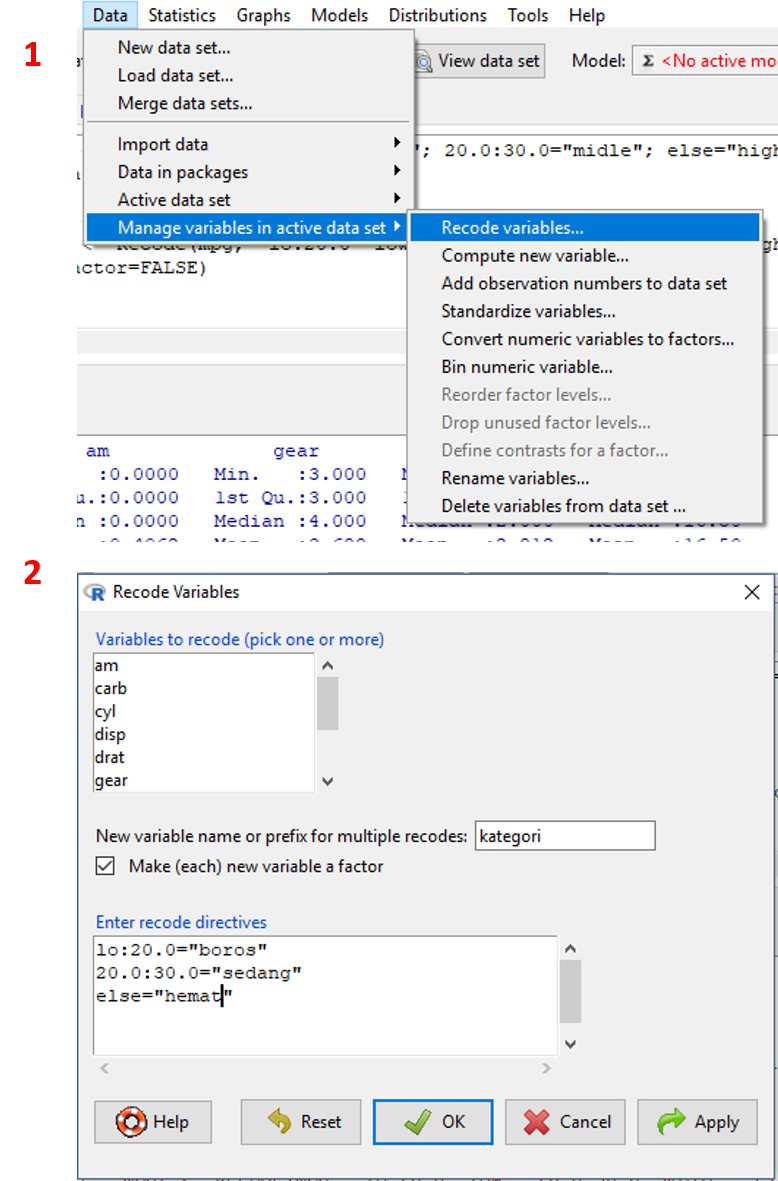
\includegraphics[width=0.7\linewidth]{./images/chp2/recodevar} 

}

\caption{Tampilan tahapan recoding variabel.}\label{fig:recode}
\end{figure}

Proses tersebut akan memunculkan sintaks pada \texttt{R\ Script} sebagai berikut:

\begin{Shaded}
\begin{Highlighting}[]
\NormalTok{mtcars <-}\StringTok{ }\KeywordTok{within}\NormalTok{(mtcars, \{kategori <-}\StringTok{ }\KeywordTok{Recode}\NormalTok{(mpg,}
          \StringTok{`}\DataTypeTok{lo:20.0="boros"; 20.0:30.0="sedang"; else="hemat"; ;',}
\DataTypeTok{          as.factor=TRUE)}
\DataTypeTok{\})}
\end{Highlighting}
\end{Shaded}

\begin{longtable}[]{@{}llll@{}}
\caption{\label{tab:recodevar2} Penjelasan item jendela Recode Variables.}\tabularnewline
\toprule
\begin{minipage}[b]{0.07\columnwidth}\raggedright
\textbf{No.}\strut
\end{minipage} & \begin{minipage}[b]{0.23\columnwidth}\raggedright
\textbf{Item}\strut
\end{minipage} & \begin{minipage}[b]{0.15\columnwidth}\raggedright
\textbf{Jenis Input}\strut
\end{minipage} & \begin{minipage}[b]{0.43\columnwidth}\raggedright
\textbf{Keterangan}\strut
\end{minipage}\tabularnewline
\midrule
\endfirsthead
\toprule
\begin{minipage}[b]{0.07\columnwidth}\raggedright
\textbf{No.}\strut
\end{minipage} & \begin{minipage}[b]{0.23\columnwidth}\raggedright
\textbf{Item}\strut
\end{minipage} & \begin{minipage}[b]{0.15\columnwidth}\raggedright
\textbf{Jenis Input}\strut
\end{minipage} & \begin{minipage}[b]{0.43\columnwidth}\raggedright
\textbf{Keterangan}\strut
\end{minipage}\tabularnewline
\midrule
\endhead
\begin{minipage}[t]{0.07\columnwidth}\raggedright
1.\strut
\end{minipage} & \begin{minipage}[t]{0.23\columnwidth}\raggedright
Variables to recode\strut
\end{minipage} & \begin{minipage}[t]{0.15\columnwidth}\raggedright
\emph{select box}\strut
\end{minipage} & \begin{minipage}[t]{0.43\columnwidth}\raggedright
daftar nama variabel yang akan di \emph{recode}\strut
\end{minipage}\tabularnewline
\begin{minipage}[t]{0.07\columnwidth}\raggedright
2.\strut
\end{minipage} & \begin{minipage}[t]{0.23\columnwidth}\raggedright
New variable name or..\strut
\end{minipage} & \begin{minipage}[t]{0.15\columnwidth}\raggedright
\emph{text input}\strut
\end{minipage} & \begin{minipage}[t]{0.43\columnwidth}\raggedright
nama baru untuk variabel yang dibuat\strut
\end{minipage}\tabularnewline
\begin{minipage}[t]{0.07\columnwidth}\raggedright
3.\strut
\end{minipage} & \begin{minipage}[t]{0.23\columnwidth}\raggedright
Make (each) variable..\strut
\end{minipage} & \begin{minipage}[t]{0.15\columnwidth}\raggedright
\emph{check box}\strut
\end{minipage} & \begin{minipage}[t]{0.43\columnwidth}\raggedright
pilihan apakah variabel baru adalah factor\strut
\end{minipage}\tabularnewline
\begin{minipage}[t]{0.07\columnwidth}\raggedright
4.\strut
\end{minipage} & \begin{minipage}[t]{0.23\columnwidth}\raggedright
Enter recode directives\strut
\end{minipage} & \begin{minipage}[t]{0.15\columnwidth}\raggedright
\emph{text input}\strut
\end{minipage} & \begin{minipage}[t]{0.43\columnwidth}\raggedright
kotak untuk memasukkan ketentuan \emph{recode}\strut
\end{minipage}\tabularnewline
\bottomrule
\end{longtable}

\hypertarget{komputasi-variabel-baru}{%
\subsection{Komputasi Variabel Baru}\label{komputasi-variabel-baru}}

Pada saat analisis data, variabel yang kita miliki terkadang tidak cukup untuk menjelaskan suatu fenomena. Namun, kita dapat membentuk sebuah variabel baru yang dapat membantu menjelaskan fenomena tersebut. Pembentukan variabel baru dapat berupa tranformasi sebuah variabel atau pembentukan variabel berdasarkan beberapa formulasi beberapa variabel lain.

Dalam melakukan tranformasi variabel, kita dapat memanfaatkan sejumlah operator operasi yang telah penulis jelaskan pada Chapter \ref{aritmatikop}. Selain operator tersebut, terdapat sejumlah fungsi operasi arimatika yang tersedia pada \texttt{R}. Fungsi-fungsi tersebut, antara lain:

\begin{enumerate}
\def\labelenumi{\arabic{enumi}.}
\tightlist
\item
  Logaritma dan eksponensial
\end{enumerate}

Untuk contoh fungsi logaritmik dan eksponensial jalankan sintaks berikut:

\begin{Shaded}
\begin{Highlighting}[]
\KeywordTok{log2}\NormalTok{(}\DecValTok{8}\NormalTok{) }\CommentTok{# logaritma basis 2 untuk 8}
\end{Highlighting}
\end{Shaded}

\begin{verbatim}
## [1] 3
\end{verbatim}

\begin{Shaded}
\begin{Highlighting}[]
\KeywordTok{log10}\NormalTok{(}\DecValTok{8}\NormalTok{) }\CommentTok{# logaritma basis 10 untuk 8}
\end{Highlighting}
\end{Shaded}

\begin{verbatim}
## [1] 0.9031
\end{verbatim}

\begin{Shaded}
\begin{Highlighting}[]
\KeywordTok{exp}\NormalTok{(}\DecValTok{8}\NormalTok{) }\CommentTok{# eksponensial 8}
\end{Highlighting}
\end{Shaded}

\begin{verbatim}
## [1] 2981
\end{verbatim}

\begin{enumerate}
\def\labelenumi{\arabic{enumi}.}
\setcounter{enumi}{1}
\tightlist
\item
  Fungsi trigonometri
\end{enumerate}

fungsi trigonometri yang ditampilkan seperti sin,cos, tan, dll.

\begin{Shaded}
\begin{Highlighting}[]
\KeywordTok{cos}\NormalTok{(x) }\CommentTok{# cos x}
\KeywordTok{sin}\NormalTok{(x) }\CommentTok{# Sin x}
\KeywordTok{tan}\NormalTok{(x) }\CommentTok{# Tan x}
\KeywordTok{acos}\NormalTok{(x) }\CommentTok{# arc-cos x}
\KeywordTok{asin}\NormalTok{(x) }\CommentTok{# arc-sin x}
\KeywordTok{atan}\NormalTok{(x) }\CommentTok{#arc-tan x}
\end{Highlighting}
\end{Shaded}

\begin{quote}
**PENTING!!!: x dalam fungsi trigonometri memiliki satuan radian
\end{quote}

Berikut adalah salah satu contoh penggunaannya:

\begin{Shaded}
\begin{Highlighting}[]
\KeywordTok{cos}\NormalTok{(pi)}
\end{Highlighting}
\end{Shaded}

\begin{verbatim}
## [1] -1
\end{verbatim}

\begin{enumerate}
\def\labelenumi{\arabic{enumi}.}
\setcounter{enumi}{2}
\tightlist
\item
  Fungsi matematik lainnya
\end{enumerate}

Fungsi lainnya yang dapat digunakan adalah fungsi absolut, akar kuadrat, dll. Berikut adalah contoh sintaks penggunaan fungsi absolut dan akar kuadrat.

\begin{Shaded}
\begin{Highlighting}[]
\KeywordTok{abs}\NormalTok{(}\OperatorTok{-}\DecValTok{2}\NormalTok{) }\CommentTok{# nilai absolut -2}
\end{Highlighting}
\end{Shaded}

\begin{verbatim}
## [1] 2
\end{verbatim}

\begin{Shaded}
\begin{Highlighting}[]
\KeywordTok{sqrt}\NormalTok{(}\DecValTok{4}\NormalTok{) }\CommentTok{# akar kuadrat 4}
\end{Highlighting}
\end{Shaded}

\begin{verbatim}
## [1] 2
\end{verbatim}

Untuk memahami permasalahan terkait komputasi variabel baru, kita akan membuat variabel baru pada dataset \texttt{mtcars} yang telah dijelaskan pada Tabel \ref{tab:mtcars}. Variabel baru yang akan kita buat adalah variabel rasio antara jarak tempuh per satuan bahan bakar (\texttt{mpg}) terhadap berat kendaraan (\texttt{wt}) dan kita namai variabel baru tersebut \texttt{rwt}. Variabel baru ini dapat menjadi alternatif lain dalam menjelaskan efisiensi suatu mobil yang ditandai dengan rasio antara jarak tempuh terhadap bobot dan konsumsi bahan bakarnya. Berikut adalah tahapan untuk melakukannya:

\begin{enumerate}
\def\labelenumi{\arabic{enumi}.}
\tightlist
\item
  Pada menu \texttt{Data}, klik \texttt{Data/Manage\ variables\ in\ active\ data\ set/Compute\ new\ variable}.
\item
  Pada jendela yang muncul, ketikkan formula pembentuk variabel baru pada kotak \texttt{Expression\ to\ compute}.
\item
  Untuk memasukkan nama variabel ke dalam formula, pembaca dapat mengetikkan nama variabel secara manual atau melakukan \emph{double click} nama variabel yang tersedia pada kotak \texttt{Current\ variables}.
\item
  Ketikkan nama variabel baru pada kotak \texttt{New\ variable\ name}. Klik \texttt{OK}.
\item
  Untuk mengecek variabel yang telah terbentuk, klik \texttt{View\ data\ set}.
\end{enumerate}

Visualisasi tahapan tersebut ditampilkan pada Gambar \ref{fig:computevar}.

\begin{figure}

{\centering 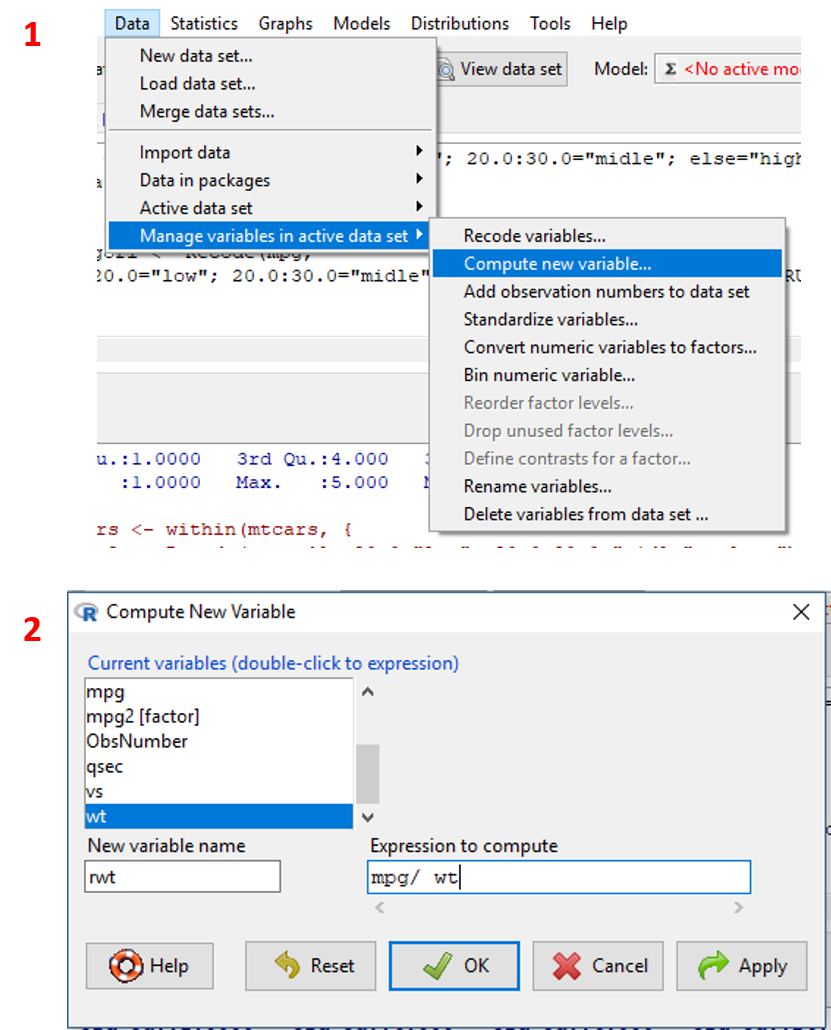
\includegraphics[width=0.7\linewidth]{./images/chp2/computevar} 

}

\caption{Tampilan tahapan komputasi variabel baru.}\label{fig:computevar}
\end{figure}

Berdasarkan tahapan tersebut, sintaks yang terbentuk pada \texttt{R\ Script} adalah sebagai berikut:

\begin{Shaded}
\begin{Highlighting}[]
\NormalTok{mtcars}\OperatorTok{$}\NormalTok{rwt <-}\StringTok{ }\KeywordTok{with}\NormalTok{(mtcars, mpg}\OperatorTok{/}\StringTok{ }\NormalTok{wt)}
\end{Highlighting}
\end{Shaded}

\hypertarget{menambahkan-variabel-nomor-observasi-pada-dataset}{%
\subsection{Menambahkan Variabel Nomor Observasi Pada Dataset}\label{menambahkan-variabel-nomor-observasi-pada-dataset}}

Untuk menambahkan variabel nomor observasi pada dataset jalankan langkah-langkah berikut:

\begin{enumerate}
\def\labelenumi{\arabic{enumi}.}
\tightlist
\item
  Pada menu \texttt{Data}, klik \texttt{Data/Manage\ variables\ in\ active\ data\ set/Add\ observation\ numbers\ to\ data\ set}.
\item
  Variabel \texttt{ObsNumber} berupa nomor observasi akan secara otomatis ditambahkan pada akhir kolom dataset.
\item
  Untuk mengecek variabel baru tersebut, klik \emph{toolbar} \texttt{View\ data\ set}.
\end{enumerate}

Pada akhir tahapan, sintaks berikut tercetak pada \texttt{R\ Script}:

\begin{Shaded}
\begin{Highlighting}[]
\NormalTok{dataset}\OperatorTok{$}\NormalTok{ObsNumber <-}\StringTok{ }\DecValTok{1}\OperatorTok{:}\StringTok{"number of observation"}
\end{Highlighting}
\end{Shaded}

\hypertarget{standardisasi-variabel}{%
\subsection{Standardisasi Variabel}\label{standardisasi-variabel}}

Standardisasi variabel bertujuan untuk mentransformasi variabel sehingga variabel tersebut memiliki nilai rata-rata 0 dan simpangan baku 1. Tahapan melakukan standardisasi variabel pada \texttt{R\ Commander} adalah sebagai berikut:

\begin{enumerate}
\def\labelenumi{\arabic{enumi}.}
\tightlist
\item
  Pada menu \texttt{Data}, klik \texttt{Data/Manage\ variables\ in\ active\ data\ set/Standardize\ variables...}.
\item
  Pada jendela yang muncul, pilih variabel yang akan di standardisasi. Pembaca dapat memilih lebih dari satu variabel dengan cara menekan tombol ctrl+klik (pada Windows) saat memilih variabel. Klik \texttt{OK}.
\item
  Untuk mengecek variabel yang telah distandadrdisasi, klik \emph{toolbar} \texttt{View\ data\ set}.
\end{enumerate}

Visualisasi tahapan tersebut ditampilkan pada Gambar \ref{fig:stanvar}.

\begin{figure}

{\centering 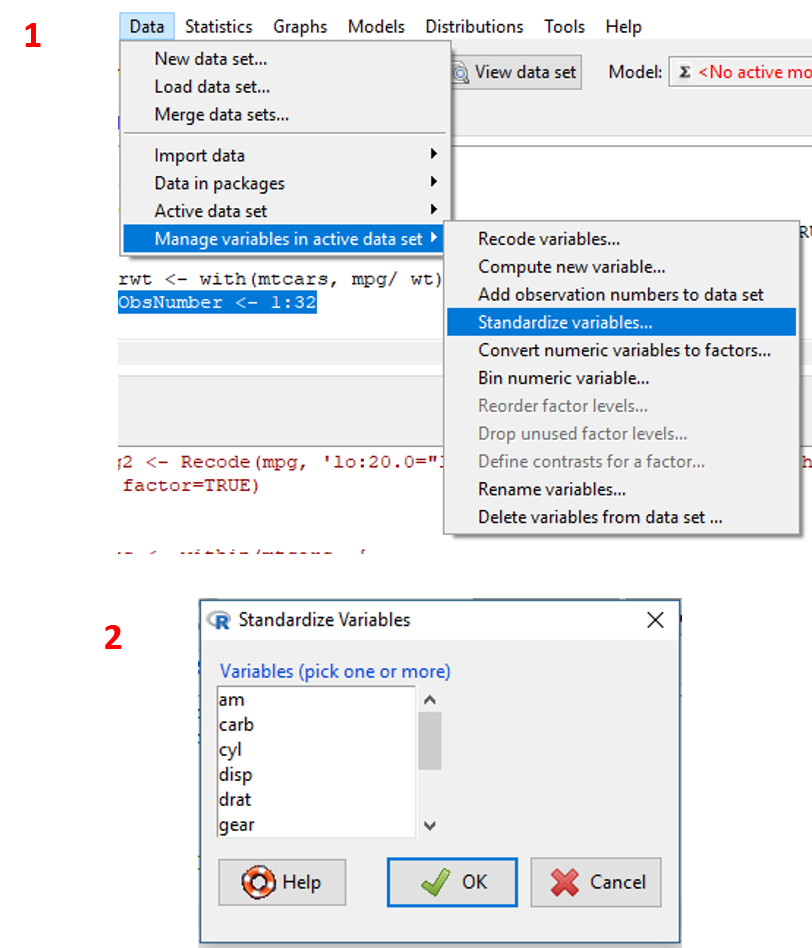
\includegraphics[width=0.7\linewidth]{./images/chp2/stanvar} 

}

\caption{Tampilan tahapan standardisasi variabel.}\label{fig:stanvar}
\end{figure}

Sintaks yang digunakan dalam tahapan tersebut adalah sebagai berikut:

\begin{Shaded}
\begin{Highlighting}[]
\NormalTok{dataset <-}\StringTok{ }\KeywordTok{local}\NormalTok{(\{}
\NormalTok{  .Z <-}\StringTok{ }\KeywordTok{scale}\NormalTok{(dataset[,}\KeywordTok{c}\NormalTok{(}\StringTok{"namavariabel"}\NormalTok{)])}
  \KeywordTok{within}\NormalTok{(dataset, \{}
\NormalTok{    Z.namavariabel <-}\StringTok{ }\NormalTok{.Z[,nomor_kolom_variabel] }
\NormalTok{  \})}
\NormalTok{\})}
\end{Highlighting}
\end{Shaded}

\hypertarget{numfac}{%
\subsection{\texorpdfstring{Merubah Variabel \emph{Numeric} Menjadi \emph{Factor}}{Merubah Variabel Numeric Menjadi Factor}}\label{numfac}}

Pada Chapter \ref{revar}, kita telah belajar bagaimana cara melakukan \emph{recoding} variabel dan membentuk \emph{factor}. Pada Chapter \ref{numfac}, kita akan membahas cara merubah variabel \emph{numeric} menjadi \emph{factor} tanpa perlu melakukan proses \emph{recoding}. Pada Chapter ini, kita hanya perlu mesuplai variabel \emph{numeric} yang akan diubah menjadi \emph{factor}. Kita juga dapat menambahkan label pada \emph{factor} tersebut. Untuk melakukannya jalankan langkah-langkah berikut:

\begin{enumerate}
\def\labelenumi{\arabic{enumi}.}
\tightlist
\item
  Pada menu \texttt{Data}, klik \texttt{Data/Manage\ variables\ in\ active\ data\ set/Convert\ numeric\ varibles\ to\ factors}.
\item
  Spesifikasikan variabel yang akan diubah menjadi \emph{factor} (lihat Tabel \ref{tab:numtofac2}). Klik \texttt{OK}
\item
  Untuk mengecek apakah variabel telah terkonversi menjadi \emph{factor}, klik \texttt{Statistics/Summaries/Active\ data\ set}. Variabel yang telah dikonversi menjadi \emph{factor} akan memberikan ringkasan data berupa tabel kontingensi (tidak menampilkan mean, min, max, dll).
\end{enumerate}

Visualisasi tahapan tersebut ditampilkan pada Gambar \ref{fig:numtofac}.

\begin{figure}

{\centering 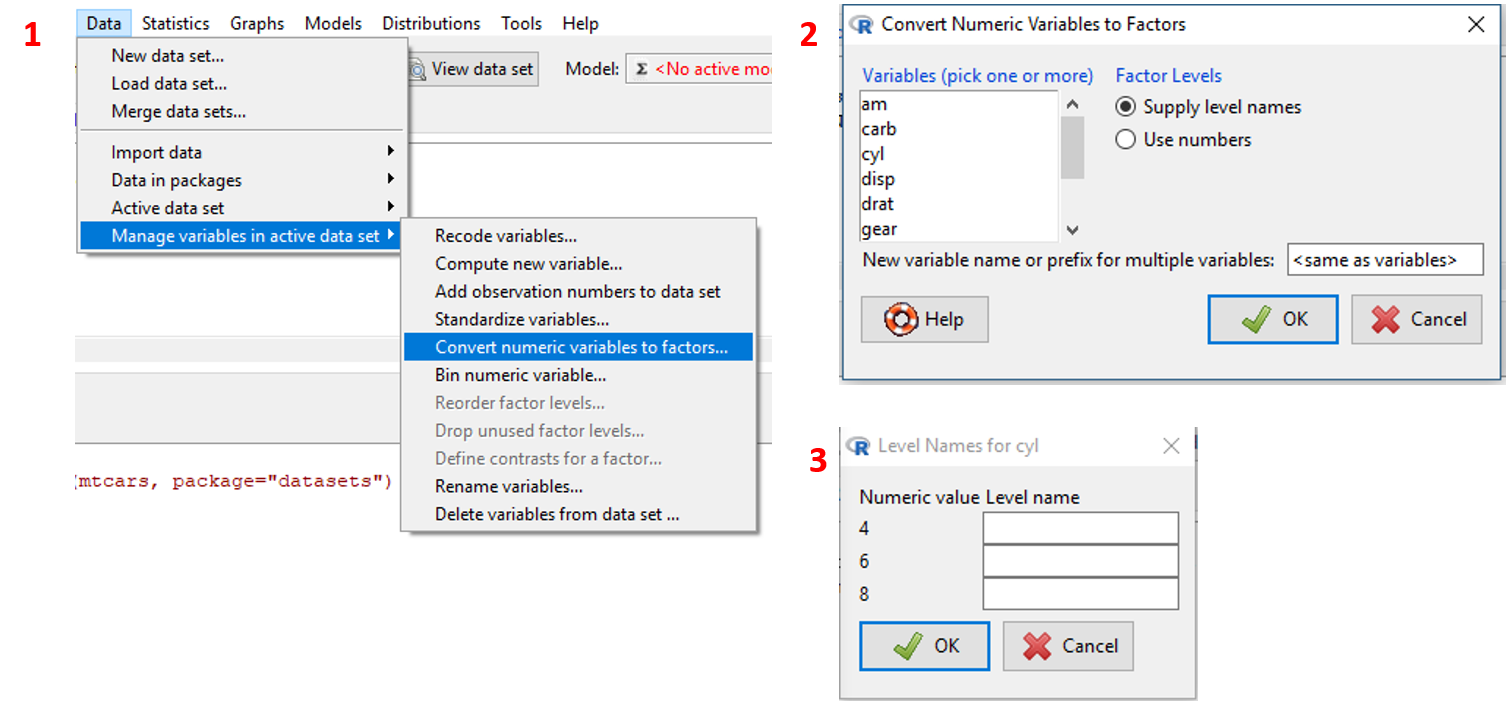
\includegraphics[width=0.7\linewidth]{./images/chp2/numtofac} 

}

\caption{Tampilan tahapan merubah variabel numeric menjadi factor.}\label{fig:numtofac}
\end{figure}

Sintaks yang dihasilkan pada proses tersebut adalah sebagai berikut:

\begin{Shaded}
\begin{Highlighting}[]
\CommentTok{# use numbers}
\NormalTok{dataset <-}\StringTok{ }\KeywordTok{within}\NormalTok{(dataset, \{}
\NormalTok{  namavariabel <-}\StringTok{ }\KeywordTok{as.factor}\NormalTok{(namavariabel)}
\NormalTok{\})}

\CommentTok{# supply level names}
\NormalTok{dataset<-}\StringTok{ }\KeywordTok{within}\NormalTok{(dataset, \{}
\NormalTok{  namavariabel <-}\StringTok{ }\KeywordTok{factor}\NormalTok{(namavariabel, }
                         \DataTypeTok{labels=}\KeywordTok{c}\NormalTok{(}\StringTok{'label1'}\NormalTok{,}\StringTok{'label2'}\NormalTok{,...))}
\NormalTok{\})}
\end{Highlighting}
\end{Shaded}

\begin{longtable}[]{@{}llll@{}}
\caption{\label{tab:numtofac2} Penjelasan item convert numeric variables to factors.}\tabularnewline
\toprule
\begin{minipage}[b]{0.04\columnwidth}\raggedright
\textbf{No.}\strut
\end{minipage} & \begin{minipage}[b]{0.14\columnwidth}\raggedright
\textbf{Item}\strut
\end{minipage} & \begin{minipage}[b]{0.09\columnwidth}\raggedright
\textbf{Jenis Input}\strut
\end{minipage} & \begin{minipage}[b]{0.61\columnwidth}\raggedright
\textbf{Keterangan}\strut
\end{minipage}\tabularnewline
\midrule
\endfirsthead
\toprule
\begin{minipage}[b]{0.04\columnwidth}\raggedright
\textbf{No.}\strut
\end{minipage} & \begin{minipage}[b]{0.14\columnwidth}\raggedright
\textbf{Item}\strut
\end{minipage} & \begin{minipage}[b]{0.09\columnwidth}\raggedright
\textbf{Jenis Input}\strut
\end{minipage} & \begin{minipage}[b]{0.61\columnwidth}\raggedright
\textbf{Keterangan}\strut
\end{minipage}\tabularnewline
\midrule
\endhead
\begin{minipage}[t]{0.04\columnwidth}\raggedright
1.\strut
\end{minipage} & \begin{minipage}[t]{0.14\columnwidth}\raggedright
Variables\strut
\end{minipage} & \begin{minipage}[t]{0.09\columnwidth}\raggedright
\emph{select box}\strut
\end{minipage} & \begin{minipage}[t]{0.61\columnwidth}\raggedright
daftar nama variabel yang akan diubah menjadi \emph{factor}\strut
\end{minipage}\tabularnewline
\begin{minipage}[t]{0.04\columnwidth}\raggedright
2.\strut
\end{minipage} & \begin{minipage}[t]{0.14\columnwidth}\raggedright
Factor levels\strut
\end{minipage} & \begin{minipage}[t]{0.09\columnwidth}\raggedright
\emph{radio button}\strut
\end{minipage} & \begin{minipage}[t]{0.61\columnwidth}\raggedright
pilihan apakah perlu menambahkan label pada \emph{factor} atau tidak\strut
\end{minipage}\tabularnewline
\begin{minipage}[t]{0.04\columnwidth}\raggedright
3.\strut
\end{minipage} & \begin{minipage}[t]{0.14\columnwidth}\raggedright
New variable name or\ldots{}\strut
\end{minipage} & \begin{minipage}[t]{0.09\columnwidth}\raggedright
\emph{text input}\strut
\end{minipage} & \begin{minipage}[t]{0.61\columnwidth}\raggedright
jika tidak diisi maka variabel lama akan diganti variabel baru (tidak ada variabel baru ditambahkan)\strut
\end{minipage}\tabularnewline
\bottomrule
\end{longtable}

\hypertarget{melakukan-binning-pada-variabel-numeric}{%
\subsection{\texorpdfstring{Melakukan \emph{Binning} pada Variabel \emph{Numeric}}{Melakukan Binning pada Variabel Numeric}}\label{melakukan-binning-pada-variabel-numeric}}

\emph{Binning} variabel numeric merupakan cara untuk mengelompokkan nilai variabel \emph{numeric} ke dalam suatu kelas berdasarkan rentang tertentu. Penetapan rentang pada proses \emph{binning} di \texttt{R\ Commander} terbagi atas 3 metode, yaitu:

\begin{itemize}
\tightlist
\item
  \textbf{\emph{Equal-width}} : membagi data ke dalam kelas berdasarkan interval yang seragam.
\item
  \textbf{\emph{Equal-count}} : membagi data ke dalam kelas berdasarkan jumlah kelas yang sama.
\item
  \textbf{\emph{Natural break}} : membagi data ke dalam kelas berdasarkan jarak terdekat (biasanya menggunakan jarak Euclidian) pada pusat masing-masing kelas. Algoritma pengelompokan yang biasa digunakan adalah algoritma \emph{k-means} (baca \href{https://id.wikipedia.org/wiki/K-means}{K-Means}).
\end{itemize}

Tahapan untuk melakukan proses \emph{binning} variabel numeric antara lain:

\begin{enumerate}
\def\labelenumi{\arabic{enumi}.}
\tightlist
\item
  Pada menu \texttt{Data}, klik \texttt{Data/Manage\ variables\ in\ active\ data\ set/Bin\ numeric\ variable...}.
\item
  Pada jendela yang muncul spesifikasikan variabel numeric yang akan di \emph{binning} dan metode pengelompokan yang digunakan (lihat Tabel \ref{tab:binvartab}. Klik \texttt{OK}.
\item
  Untuk mengecek variabel hasil \emph{binning}, klik \emph{toolbar} \texttt{View\ data\ set}.
\end{enumerate}

Visualisasi tahapan tersebut ditampilkan pada Gambar \ref{fig:binvar}.

\begin{figure}

{\centering 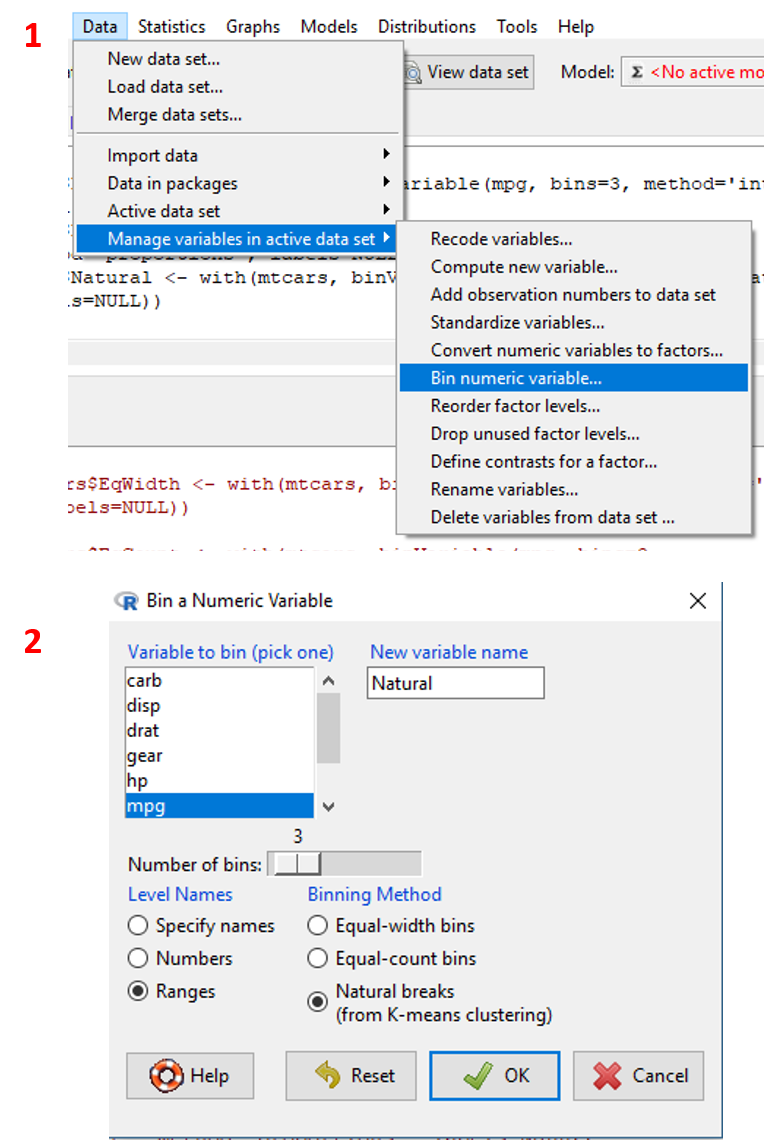
\includegraphics[width=0.7\linewidth]{./images/chp2/binvar} 

}

\caption{Tampilan tahapan binning variabel numeric.}\label{fig:binvar}
\end{figure}

Sintaks yang digunakan pada masing-masing metode \emph{binning}, antara lain:

\begin{Shaded}
\begin{Highlighting}[]
\CommentTok{# Equal-width}
\NormalTok{dataset}\OperatorTok{$}\NormalTok{namavariabel <-}\StringTok{ }\KeywordTok{with}\NormalTok{(dataset, }\KeywordTok{binVariable}\NormalTok{(variabel, }
                        \DataTypeTok{bins=}\StringTok{"jumlah_bin"}\NormalTok{, }\DataTypeTok{method=}\StringTok{'intervals'}\NormalTok{,}
                        \DataTypeTok{labels=}\KeywordTok{c}\NormalTok{(}\StringTok{"label1"}\NormalTok{,...)))}
\NormalTok{dataset}\OperatorTok{$}\NormalTok{namavariabel <-}\StringTok{ }\KeywordTok{with}\NormalTok{(dataset, }\KeywordTok{binVariable}\NormalTok{(variabel, }
                        \DataTypeTok{bins=}\StringTok{"jumlah_bin"}\NormalTok{, }\DataTypeTok{method=}\StringTok{'proportions'}\NormalTok{, }
                        \DataTypeTok{labels=}\KeywordTok{c}\NormalTok{(}\StringTok{"label1"}\NormalTok{,...)))}
\NormalTok{dataset}\OperatorTok{$}\NormalTok{namavariabel <-}\StringTok{ }\KeywordTok{with}\NormalTok{(dataset, }\KeywordTok{binVariable}\NormalTok{(variabel, }
                        \DataTypeTok{bins=}\StringTok{"jumlah_bin"}\NormalTok{, }\DataTypeTok{method=}\StringTok{'natural'}\NormalTok{,}
                        \DataTypeTok{labels=}\KeywordTok{c}\NormalTok{(}\StringTok{"label1"}\NormalTok{,...)))}
\end{Highlighting}
\end{Shaded}

\begin{longtable}[]{@{}llll@{}}
\caption{\label{tab:binvartab} Penjelasan item jendela convert numeric variables to factors.}\tabularnewline
\toprule
\begin{minipage}[b]{0.04\columnwidth}\raggedright
\textbf{No.}\strut
\end{minipage} & \begin{minipage}[b]{0.14\columnwidth}\raggedright
\textbf{Item}\strut
\end{minipage} & \begin{minipage}[b]{0.09\columnwidth}\raggedright
\textbf{Jenis Input}\strut
\end{minipage} & \begin{minipage}[b]{0.61\columnwidth}\raggedright
\textbf{Keterangan}\strut
\end{minipage}\tabularnewline
\midrule
\endfirsthead
\toprule
\begin{minipage}[b]{0.04\columnwidth}\raggedright
\textbf{No.}\strut
\end{minipage} & \begin{minipage}[b]{0.14\columnwidth}\raggedright
\textbf{Item}\strut
\end{minipage} & \begin{minipage}[b]{0.09\columnwidth}\raggedright
\textbf{Jenis Input}\strut
\end{minipage} & \begin{minipage}[b]{0.61\columnwidth}\raggedright
\textbf{Keterangan}\strut
\end{minipage}\tabularnewline
\midrule
\endhead
\begin{minipage}[t]{0.04\columnwidth}\raggedright
1.\strut
\end{minipage} & \begin{minipage}[t]{0.14\columnwidth}\raggedright
Variables to bin\strut
\end{minipage} & \begin{minipage}[t]{0.09\columnwidth}\raggedright
\emph{select box}\strut
\end{minipage} & \begin{minipage}[t]{0.61\columnwidth}\raggedright
daftar nama variabel \emph{numeric} yang akan dilakukan \emph{binning}\strut
\end{minipage}\tabularnewline
\begin{minipage}[t]{0.04\columnwidth}\raggedright
2.\strut
\end{minipage} & \begin{minipage}[t]{0.14\columnwidth}\raggedright
New variable name\strut
\end{minipage} & \begin{minipage}[t]{0.09\columnwidth}\raggedright
\emph{text input}\strut
\end{minipage} & \begin{minipage}[t]{0.61\columnwidth}\raggedright
Input nama variabel baru\strut
\end{minipage}\tabularnewline
\begin{minipage}[t]{0.04\columnwidth}\raggedright
3.\strut
\end{minipage} & \begin{minipage}[t]{0.14\columnwidth}\raggedright
Number of bins\strut
\end{minipage} & \begin{minipage}[t]{0.09\columnwidth}\raggedright
\emph{slider}\strut
\end{minipage} & \begin{minipage}[t]{0.61\columnwidth}\raggedright
spesifikasi jumlah bin atau kelas yang digunakan\strut
\end{minipage}\tabularnewline
\begin{minipage}[t]{0.04\columnwidth}\raggedright
4.\strut
\end{minipage} & \begin{minipage}[t]{0.14\columnwidth}\raggedright
Level Names\strut
\end{minipage} & \begin{minipage}[t]{0.09\columnwidth}\raggedright
\emph{radio button}\strut
\end{minipage} & \begin{minipage}[t]{0.61\columnwidth}\raggedright
spesifikasi metode penamaan bin\strut
\end{minipage}\tabularnewline
\begin{minipage}[t]{0.04\columnwidth}\raggedright
5.\strut
\end{minipage} & \begin{minipage}[t]{0.14\columnwidth}\raggedright
Binning Method\strut
\end{minipage} & \begin{minipage}[t]{0.09\columnwidth}\raggedright
\emph{radio button}\strut
\end{minipage} & \begin{minipage}[t]{0.61\columnwidth}\raggedright
spesifikasi metode \emph{binning}\strut
\end{minipage}\tabularnewline
\bottomrule
\end{longtable}

\hypertarget{merubah-urutan-factor-levels}{%
\subsection{\texorpdfstring{Merubah Urutan \emph{Factor Levels}}{Merubah Urutan Factor Levels}}\label{merubah-urutan-factor-levels}}

Secara umum saat kita merubah sebuah variabel \emph{character} atau \emph{string} menjadi \emph{factor} level \emph{factor} hasil konversi tersebut diurutkan berdasarkan abjad. Sebuah variabel yang terdiri dari nilai ``setuju'', ``netral'', dan ``tidak setuju'', jika diubah menjadi \emph{factor} akan memiliki urutan level ``netral'', ``setuju'', dan ``tidak setuju''. Urutan tersebut tidak benar dan perlu dirubah. Untuk melakukannya pada \texttt{R\ Commander} jalankan langkah-langkah berikut:

\begin{enumerate}
\def\labelenumi{\arabic{enumi}.}
\tightlist
\item
  Pada menu \texttt{Data}, klik \texttt{Data/Manage\ variables\ in\ active\ data\ set/Reorder\ factor\ levels...}.
\item
  Pada jendela yang muncul spesifikasikan variable \emph{factor} yang akan dirubah (lihat Tabel \ref{tab:reofac}. Klik \texttt{OK}.
\item
  Pada jendela yang muncul, rubah urutan \emph{factor} lama. Klik \texttt{OK}.
\item
  Untuk mengecek \emph{factor level}, jalankan sintaks berikut:
\end{enumerate}

\begin{Shaded}
\begin{Highlighting}[]
\CommentTok{# ubah nama dataset dan variabel}
\KeywordTok{levels}\NormalTok{(dataset}\OperatorTok{$}\NormalTok{namavariabel)}
\end{Highlighting}
\end{Shaded}

Visualisasi tahapan tersebut ditampilkan pada Gambar \ref{fig:reorderfac}.

\begin{figure}

{\centering 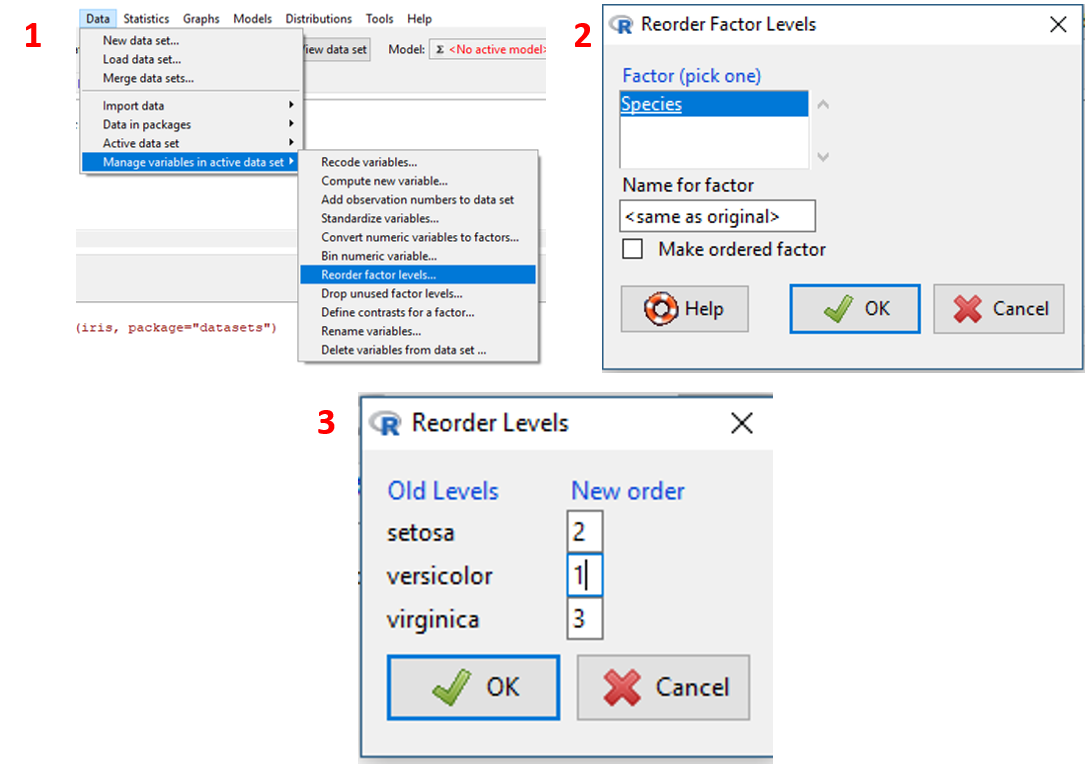
\includegraphics[width=0.7\linewidth]{./images/chp2/reorderfac} 

}

\caption{Tampilan tahapan merubah urutan factor level.}\label{fig:reorderfac}
\end{figure}

Sintaks dari tahapan merubah urutan \emph{factor} secara umum ditampilkan sebagai berikut:

\begin{Shaded}
\begin{Highlighting}[]
\NormalTok{dataset}\OperatorTok{$}\NormalTok{namavariabel <-}\StringTok{ }\KeywordTok{with}\NormalTok{(dataset, }\KeywordTok{factor}\NormalTok{(namavariabel, }
                                  \DataTypeTok{levels=}\KeywordTok{c}\NormalTok{(}\StringTok{'level1'}\NormalTok{,}
                                            \StringTok{'level2'}\NormalTok{,}
\NormalTok{                                            ....), }
                            \DataTypeTok{ordered=}\OtherTok{TRUE}\NormalTok{))}
\end{Highlighting}
\end{Shaded}

\begin{longtable}[]{@{}llll@{}}
\caption{\label{tab:reofac} Penjelasan item jendela reorder factor levels.}\tabularnewline
\toprule
\begin{minipage}[b]{0.04\columnwidth}\raggedright
\textbf{No.}\strut
\end{minipage} & \begin{minipage}[b]{0.14\columnwidth}\raggedright
\textbf{Item}\strut
\end{minipage} & \begin{minipage}[b]{0.09\columnwidth}\raggedright
\textbf{Jenis Input}\strut
\end{minipage} & \begin{minipage}[b]{0.61\columnwidth}\raggedright
\textbf{Keterangan}\strut
\end{minipage}\tabularnewline
\midrule
\endfirsthead
\toprule
\begin{minipage}[b]{0.04\columnwidth}\raggedright
\textbf{No.}\strut
\end{minipage} & \begin{minipage}[b]{0.14\columnwidth}\raggedright
\textbf{Item}\strut
\end{minipage} & \begin{minipage}[b]{0.09\columnwidth}\raggedright
\textbf{Jenis Input}\strut
\end{minipage} & \begin{minipage}[b]{0.61\columnwidth}\raggedright
\textbf{Keterangan}\strut
\end{minipage}\tabularnewline
\midrule
\endhead
\begin{minipage}[t]{0.04\columnwidth}\raggedright
1.\strut
\end{minipage} & \begin{minipage}[t]{0.14\columnwidth}\raggedright
Factor\strut
\end{minipage} & \begin{minipage}[t]{0.09\columnwidth}\raggedright
\emph{select box}\strut
\end{minipage} & \begin{minipage}[t]{0.61\columnwidth}\raggedright
daftar variabel \emph{factor} pada dataset\strut
\end{minipage}\tabularnewline
\begin{minipage}[t]{0.04\columnwidth}\raggedright
2.\strut
\end{minipage} & \begin{minipage}[t]{0.14\columnwidth}\raggedright
Name for factor\strut
\end{minipage} & \begin{minipage}[t]{0.09\columnwidth}\raggedright
\emph{text input}\strut
\end{minipage} & \begin{minipage}[t]{0.61\columnwidth}\raggedright
nama variabel \emph{factor} yang baru (jika ingin membuat variabel baru)\strut
\end{minipage}\tabularnewline
\begin{minipage}[t]{0.04\columnwidth}\raggedright
3.\strut
\end{minipage} & \begin{minipage}[t]{0.14\columnwidth}\raggedright
Make ordered factor\strut
\end{minipage} & \begin{minipage}[t]{0.09\columnwidth}\raggedright
\emph{check box}\strut
\end{minipage} & \begin{minipage}[t]{0.61\columnwidth}\raggedright
spesifikasi apakah \emph{factor} akan diurutkan atau tidak\strut
\end{minipage}\tabularnewline
\bottomrule
\end{longtable}

\hypertarget{melakukan-drop-pada-factor-levels}{%
\subsection{\texorpdfstring{Melakukan \emph{Drop} pada \emph{Factor Levels}}{Melakukan Drop pada Factor Levels}}\label{melakukan-drop-pada-factor-levels}}

Saat melakukan subset pada dataset yang akan dijelaskan pada Chapter \ref{transdata} sering kali tidak semua \emph{factor level} ada pada dataset tersebut (sejumlah \emph{factor level} memiliki observasi nol) yang berpengaruh pada analisis data yang kita lakukan. Untuk mengatasinya, kita dapat melakukan \emph{drop} pada \emph{factor level tersebut}. Untuk melakukannya, jalankan langkah-langkah berikut:

\begin{enumerate}
\def\labelenumi{\arabic{enumi}.}
\tightlist
\item
  Pada menu \texttt{Data}, klik \texttt{Data/Manage\ variables\ in\ active\ data\ set/Drop\ unused\ factor\ levels...}.
\item
  Pada jendela yang muncul spesifikasikan variable \emph{factor} yang akan didrop \emph{factor levelnya}. Klik \texttt{OK}.
\end{enumerate}

Visualisasi tahapan tersebut ditampilkan pada Gambar \ref{fig:dropfac}.

\begin{figure}

{\centering 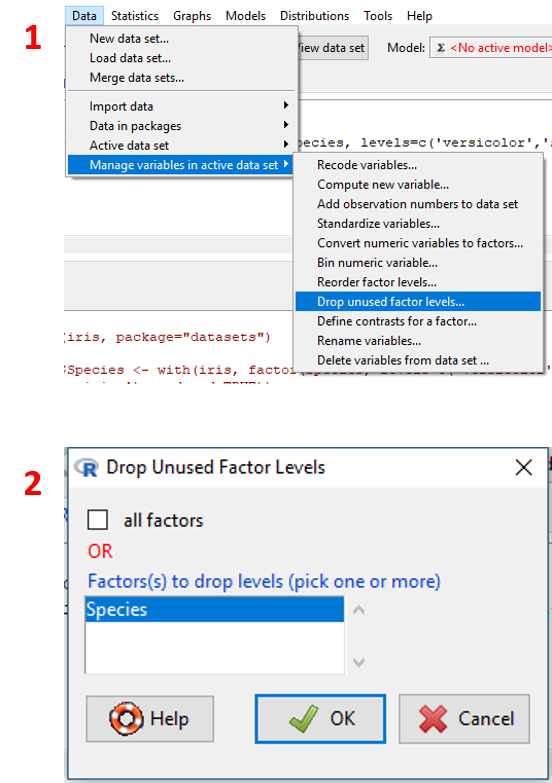
\includegraphics[width=0.7\linewidth]{./images/chp2/dropfact} 

}

\caption{Tampilan tahapan drop factor level.}\label{fig:dropfac}
\end{figure}

Sintaks untuk melakukan \emph{drop factor levels} secara umum adalah sebagai berikut:

\begin{Shaded}
\begin{Highlighting}[]
\NormalTok{dataset <-}\StringTok{ }\KeywordTok{within}\NormalTok{(dataset, \{}
\NormalTok{  namavariabel <-}\StringTok{ }\KeywordTok{droplevels}\NormalTok{(namavariabel) }
\NormalTok{\})}
\end{Highlighting}
\end{Shaded}

\hypertarget{merubah-nama-variabel-pada-data}{%
\subsection{Merubah Nama Variabel pada Data}\label{merubah-nama-variabel-pada-data}}

Untuk merubah nama variabel pada \texttt{R\ Commander} dapat dilakukan dengan dua cara, antara lain:

\textbf{Cara 1}

\begin{enumerate}
\def\labelenumi{\arabic{enumi}.}
\tightlist
\item
  Klik \emph{toolbar} \texttt{Edit\ data\ set}.
\item
  Pada jendela dataset yang muncul , \emph{double click} nama variabel yang ingin dirubah dan ubah nama variabel tersebut. Klik \texttt{OK}
\end{enumerate}

\textbf{Cara 2}

\begin{enumerate}
\def\labelenumi{\arabic{enumi}.}
\tightlist
\item
  Pada menu \texttt{Data}, klik \texttt{Data/Manage\ variables\ in\ active\ data\ set/Rename\ variables...}.
\item
  Pada jendela yang muncul pilih variabel yang ingin dirubah namanya. Klik \texttt{OK}.
\item
  Pada jendela yang muncul, isikan nama variabel baru dan Klik \texttt{OK} jika telah selesai.
\item
  Untuk mengecek apakah proses telah berhasil, klik \emph{toolbar} \texttt{View\ data\ set}.
\end{enumerate}

Visualisasi tahapan tersebut ditampilkan pada Gambar \ref{fig:renamevar}.

\begin{figure}

{\centering 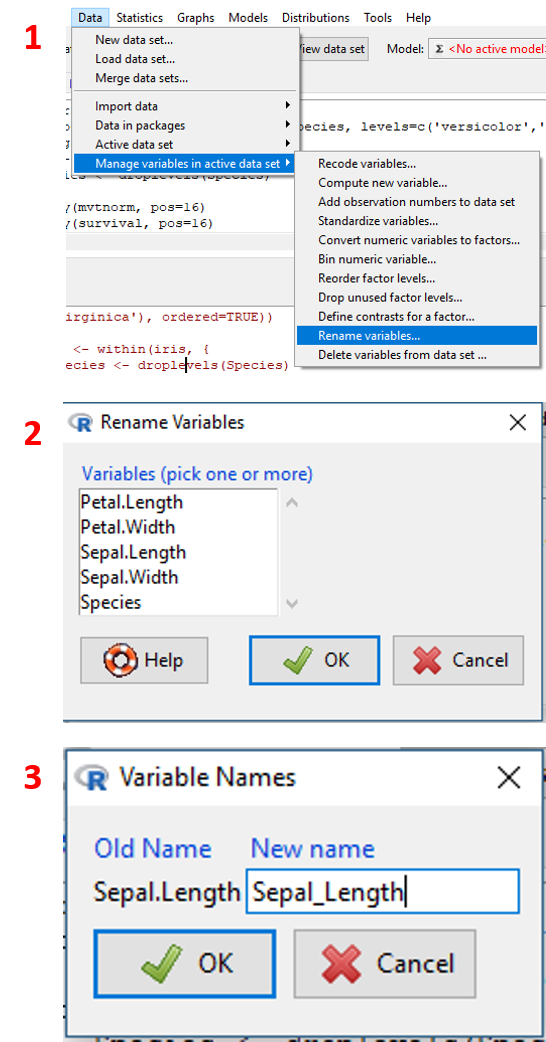
\includegraphics[width=0.7\linewidth]{./images/chp2/renamevar} 

}

\caption{Tampilan tahapan merubah nama variabel.}\label{fig:renamevar}
\end{figure}

Sintaks untuk merubah nama variabel secara umum adalah sebagai berikut:

\begin{Shaded}
\begin{Highlighting}[]
\KeywordTok{names}\NormalTok{(dataset)[}\KeywordTok{c}\NormalTok{(nomorvariabel)] <-}\StringTok{ }\KeywordTok{c}\NormalTok{(}\StringTok{"namavariabelbaru"}\NormalTok{)}
\end{Highlighting}
\end{Shaded}

\hypertarget{menghapus-variabel}{%
\subsection{Menghapus Variabel}\label{menghapus-variabel}}

Untuk menghapus variabel pada dataset, jalankan langkah-langkah berikut:

\begin{enumerate}
\def\labelenumi{\arabic{enumi}.}
\tightlist
\item
  Pada menu \texttt{Data}, klik \texttt{Data/Manage\ variables\ in\ active\ data\ set/Delete\ variables\ from\ data\ set...}.
\item
  Pada jendela yang muncul pilih variabel yang ingin dihapus. Klik \texttt{OK}.
\item
  Untuk mengecek apakah proses telah berhasil, klik \emph{toolbar} \texttt{View\ data\ set}.
\end{enumerate}

Visualisasi tahapan tersebut ditampilkan pada Gambar \ref{fig:deletevar}.

\begin{figure}

{\centering 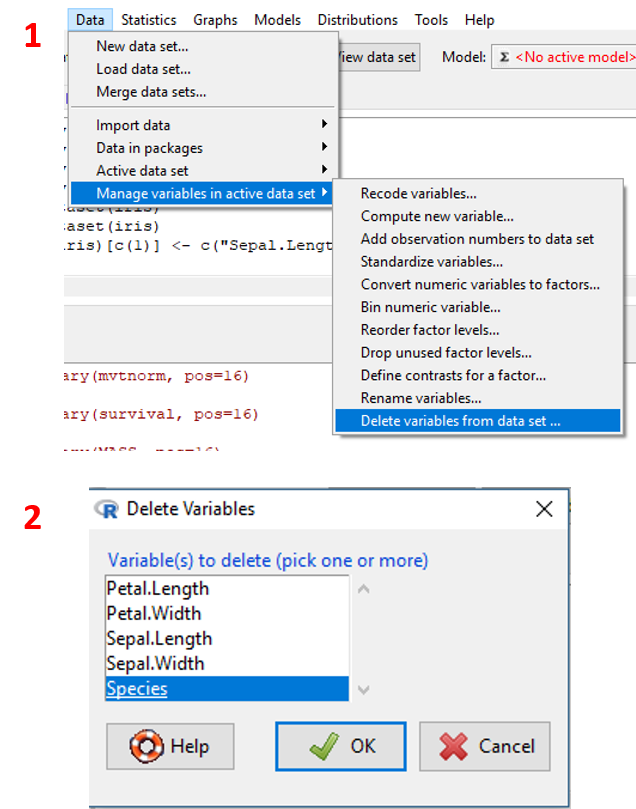
\includegraphics[width=0.7\linewidth]{./images/chp2/deletevar} 

}

\caption{Tampilan tahapan menghapus variabel.}\label{fig:deletevar}
\end{figure}

Sintaks untuk menghapus variabel secara umum adalah sebagai berikut:

\begin{Shaded}
\begin{Highlighting}[]
\NormalTok{dataset <-}\StringTok{ }\KeywordTok{within}\NormalTok{(dataset, \{}
\NormalTok{  namavariabel1 <-}\StringTok{ }\OtherTok{NULL}
\NormalTok{  namavariabel2 <-}\StringTok{ }\OtherTok{NULL} 
\NormalTok{\})}
\end{Highlighting}
\end{Shaded}

\hypertarget{transdata}{%
\section{Memanipulasi Dataset}\label{transdata}}

Pada Chapter \ref{transdata}, kita akan belajar bagaimana memanipuasi dataset. Adapun yang menjadi topik bahasan dalam Chapter \ref{transdata}, antara lain:

\begin{itemize}
\tightlist
\item
  Melakukan subset dataset,
\item
  Agregasi variabel pada dataset,
\item
  Melakukan \emph{drop} observasi pada dataset,
\item
  Melakukan \emph{drop} observasi dengan \emph{missing value},
\item
  Mengelompokkan variabel menjadi variabel \emph{factor} dan nilai,
\item
  Menggabungkan dua dataset, dan,
\item
  Modifikasi lainnya.
\end{itemize}

\hypertarget{melakukan-subset-dataset}{%
\subsection{Melakukan Subset Dataset}\label{melakukan-subset-dataset}}

Pada analisis data, kita sering kali tidak membutuhkan seluruh observasi dari data yang kita miliki. Kita akan melakukan filter untuk memperoleh data sesuai dengan keperluan kita. Selain itu, melihat subset data berdasarkan kriteria tertentu membantu kita untuk melakukan analisis ekspolarif terhadap data yang kita miliki.

Untuk melakukan subset data, kita memelukan sebuah ekpresi atau formula yang dapat mengecek satu persatu data yang memenuhi formula subset yang telah dibentuk. Sebagai contoh, kita ingin memperoleh dataset tanpa nilai \emph{missing value} pada variabel \texttt{namavariabel}. Berikut adalah contoh sintaks formula atau ekspresi yang digunakan:

\begin{Shaded}
\begin{Highlighting}[]
\OperatorTok{!}\KeywordTok{is.na}\NormalTok{(namavariabel)}
\end{Highlighting}
\end{Shaded}

Untuk membuat formula atau ekspresi tersebut, kita dapat menggunakan kembali operator operasi yang telah dijelaskan pada Chapter \ref{opop}. Langkah-langkah untuk melakukan subset pada dataset adalah sebagai berikut:

\begin{enumerate}
\def\labelenumi{\arabic{enumi}.}
\tightlist
\item
  Pada menu \texttt{Data}, klik \texttt{Data/Active\ data\ set/Subset\ active\ data\ set...}.
\item
  Pada jendela yang muncul spesifikasikan variabel yang akan dipilih pada dataset baru dan formula subset yang digunakan (lihat Tabel \ref{tab:subset}). Klik \texttt{OK}.
\item
  Untuk mengecek dataset, klik \emph{toolbar} \texttt{View\ data\ set}.
\end{enumerate}

Visualisasi tahapan tersebut ditampilkan pada Gambar \ref{fig:subsetdata}.

\begin{figure}

{\centering 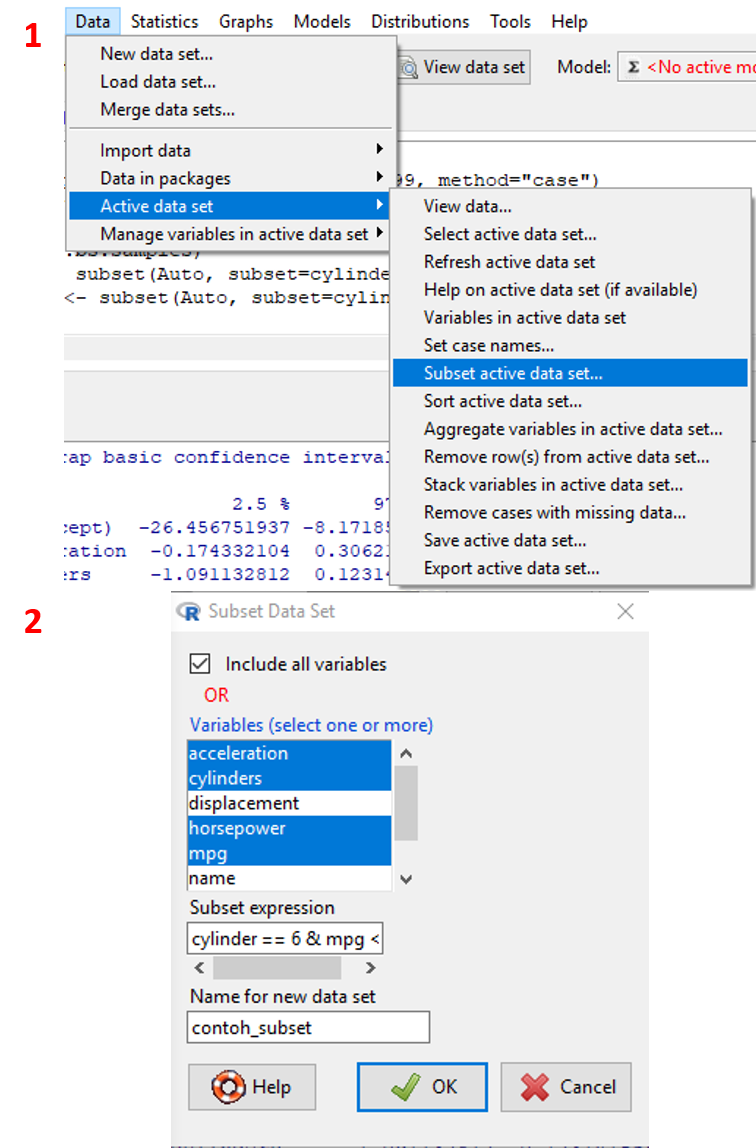
\includegraphics[width=0.7\linewidth]{./images/chp2/subsetdata} 

}

\caption{Tampilan tahapan melakukan subset pada dataset.}\label{fig:subsetdata}
\end{figure}

Secara umum sintaks untuk melakukan proses subset adalah sebagai berikut:

\begin{Shaded}
\begin{Highlighting}[]
\NormalTok{contoh_subset <-}\StringTok{ }\KeywordTok{subset}\NormalTok{(dataset,}\DataTypeTok{subset=}\NormalTok{formula_subset)}
\end{Highlighting}
\end{Shaded}

\begin{longtable}[]{@{}llll@{}}
\caption{\label{tab:subset} Penjelasan item jendela subset data set.}\tabularnewline
\toprule
\begin{minipage}[b]{0.04\columnwidth}\raggedright
\textbf{No.}\strut
\end{minipage} & \begin{minipage}[b]{0.14\columnwidth}\raggedright
\textbf{Item}\strut
\end{minipage} & \begin{minipage}[b]{0.09\columnwidth}\raggedright
\textbf{Jenis Input}\strut
\end{minipage} & \begin{minipage}[b]{0.61\columnwidth}\raggedright
\textbf{Keterangan}\strut
\end{minipage}\tabularnewline
\midrule
\endfirsthead
\toprule
\begin{minipage}[b]{0.04\columnwidth}\raggedright
\textbf{No.}\strut
\end{minipage} & \begin{minipage}[b]{0.14\columnwidth}\raggedright
\textbf{Item}\strut
\end{minipage} & \begin{minipage}[b]{0.09\columnwidth}\raggedright
\textbf{Jenis Input}\strut
\end{minipage} & \begin{minipage}[b]{0.61\columnwidth}\raggedright
\textbf{Keterangan}\strut
\end{minipage}\tabularnewline
\midrule
\endhead
\begin{minipage}[t]{0.04\columnwidth}\raggedright
1.\strut
\end{minipage} & \begin{minipage}[t]{0.14\columnwidth}\raggedright
Include all variables\strut
\end{minipage} & \begin{minipage}[t]{0.09\columnwidth}\raggedright
\emph{check box}\strut
\end{minipage} & \begin{minipage}[t]{0.61\columnwidth}\raggedright
opsi apakah akan menyertakan seluruh variabel pada hasil subset\strut
\end{minipage}\tabularnewline
\begin{minipage}[t]{0.04\columnwidth}\raggedright
2.\strut
\end{minipage} & \begin{minipage}[t]{0.14\columnwidth}\raggedright
Variables\strut
\end{minipage} & \begin{minipage}[t]{0.09\columnwidth}\raggedright
\emph{select box}\strut
\end{minipage} & \begin{minipage}[t]{0.61\columnwidth}\raggedright
daftar nama variabel yang dapat dipilih untuk ditampilkan pada hasil subset\strut
\end{minipage}\tabularnewline
\begin{minipage}[t]{0.04\columnwidth}\raggedright
3.\strut
\end{minipage} & \begin{minipage}[t]{0.14\columnwidth}\raggedright
Subset expression\strut
\end{minipage} & \begin{minipage}[t]{0.09\columnwidth}\raggedright
\emph{text input}\strut
\end{minipage} & \begin{minipage}[t]{0.61\columnwidth}\raggedright
formula atau ekpresi subset yang digunakan\strut
\end{minipage}\tabularnewline
\begin{minipage}[t]{0.04\columnwidth}\raggedright
4.\strut
\end{minipage} & \begin{minipage}[t]{0.14\columnwidth}\raggedright
Name for new data set\strut
\end{minipage} & \begin{minipage}[t]{0.09\columnwidth}\raggedright
\emph{text imput}\strut
\end{minipage} & \begin{minipage}[t]{0.61\columnwidth}\raggedright
opsi untuk memberikan nama pada dataset baru atau tidak (dataset lama akan dihapus)\strut
\end{minipage}\tabularnewline
\bottomrule
\end{longtable}

\hypertarget{agregat-variabel-pada-dataset}{%
\subsection{Agregat Variabel pada Dataset}\label{agregat-variabel-pada-dataset}}

Submenu \texttt{agregate\ variables\ in\ active\ dataset} memberikan ringkasan nilai satu atau beberapa variabel berdasarkan level variabel \emph{factor} dan menghasilkan dataset baru dengan satu observasi untuk tiap level \emph{factor}. Proses agregasi mengaplikasikan beberapa fungsi seperti \texttt{mean()}, \texttt{sum()}, atau fungsi lainnya untuk menghasilkan sebuah nilai untuk setiap observasi pada tiap variabel dan level \emph{factor}.

Fungsi statistika deskriptif bawaan yang dapat digunakan pada \texttt{R\ Commander} ditampilkan pada Tabel \ref{tab:builtinfun}.

\begin{longtable}[]{@{}ll@{}}
\caption{\label{tab:builtinfun} Fungsi statistika deskriptif bawaan pada R.}\tabularnewline
\toprule
\textbf{Fungsi} & \textbf{Keterangan}\tabularnewline
\midrule
\endfirsthead
\toprule
\textbf{Fungsi} & \textbf{Keterangan}\tabularnewline
\midrule
\endhead
\texttt{mean} & rata-rata\tabularnewline
\texttt{median} & median\tabularnewline
\texttt{sum} & jumlah seluruh observasi dalam sebuah variabel\tabularnewline
\texttt{quantile} & kuantil data\tabularnewline
\texttt{min} & nilai observasi minimum\tabularnewline
\texttt{max} & nilai observasi maksimum\tabularnewline
\texttt{IQR} & rentang antar kuartil\tabularnewline
\texttt{mad} & simpangan absolut median\tabularnewline
\texttt{sd} & simpangan baku\tabularnewline
\texttt{var} & varians\tabularnewline
\bottomrule
\end{longtable}

Tahapan agregasi variabel dilakukan melalui langkah-langkah berikut:

\begin{enumerate}
\def\labelenumi{\arabic{enumi}.}
\tightlist
\item
  Pada menu \texttt{Data}, klik \texttt{Data/Active\ data\ set/Aggregate\ variables\ in\ active\ data\ set...}.
\item
  Spesifikan variabel yang akan dilakukan agregasi, \emph{factor level} yang digunakan, dan fungsi agregat yang digunakan (lihat Tabel \ref{tab:agregat}). Klik \texttt{OK}.
\item
  Untuk mengecek dataset, klik \emph{toolbar} \texttt{View\ data\ set}.
\end{enumerate}

Visualisasi tahapan tersebut ditampilkan pada Gambar \ref{fig:agregatdata}.

\begin{figure}

{\centering 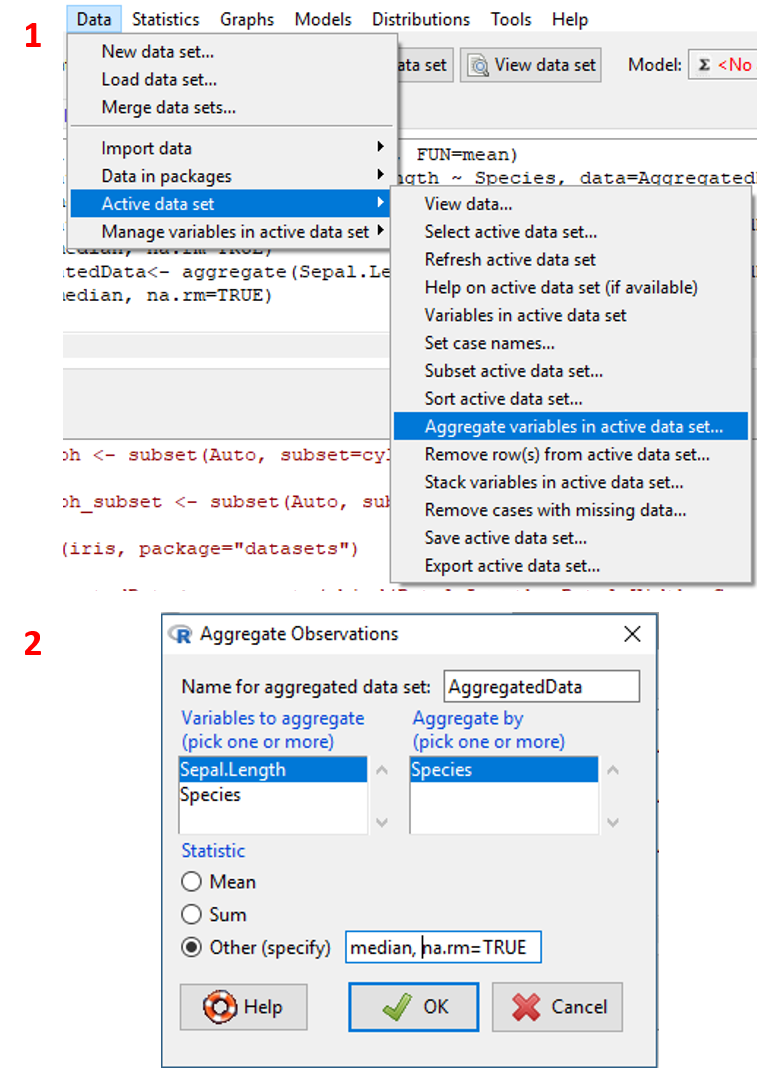
\includegraphics[width=0.7\linewidth]{./images/chp2/agregatvar} 

}

\caption{Tampilan tahapan agregasi variabel.}\label{fig:agregatdata}
\end{figure}

\begin{longtable}[]{@{}llll@{}}
\caption{\label{tab:agregat} Penjelasan item jendela aggregate observations.}\tabularnewline
\toprule
\begin{minipage}[b]{0.04\columnwidth}\raggedright
\textbf{No.}\strut
\end{minipage} & \begin{minipage}[b]{0.14\columnwidth}\raggedright
\textbf{Item}\strut
\end{minipage} & \begin{minipage}[b]{0.09\columnwidth}\raggedright
\textbf{Jenis Input}\strut
\end{minipage} & \begin{minipage}[b]{0.61\columnwidth}\raggedright
\textbf{Keterangan}\strut
\end{minipage}\tabularnewline
\midrule
\endfirsthead
\toprule
\begin{minipage}[b]{0.04\columnwidth}\raggedright
\textbf{No.}\strut
\end{minipage} & \begin{minipage}[b]{0.14\columnwidth}\raggedright
\textbf{Item}\strut
\end{minipage} & \begin{minipage}[b]{0.09\columnwidth}\raggedright
\textbf{Jenis Input}\strut
\end{minipage} & \begin{minipage}[b]{0.61\columnwidth}\raggedright
\textbf{Keterangan}\strut
\end{minipage}\tabularnewline
\midrule
\endhead
\begin{minipage}[t]{0.04\columnwidth}\raggedright
1.\strut
\end{minipage} & \begin{minipage}[t]{0.14\columnwidth}\raggedright
Name for aggregated..\strut
\end{minipage} & \begin{minipage}[t]{0.09\columnwidth}\raggedright
\emph{text input}\strut
\end{minipage} & \begin{minipage}[t]{0.61\columnwidth}\raggedright
input nama dataset baru yang dihasilkan\strut
\end{minipage}\tabularnewline
\begin{minipage}[t]{0.04\columnwidth}\raggedright
2.\strut
\end{minipage} & \begin{minipage}[t]{0.14\columnwidth}\raggedright
Variables to aggregate\strut
\end{minipage} & \begin{minipage}[t]{0.09\columnwidth}\raggedright
\emph{select box}\strut
\end{minipage} & \begin{minipage}[t]{0.61\columnwidth}\raggedright
daftar nama variabel yang dapat dipilih untuk diagregasi\strut
\end{minipage}\tabularnewline
\begin{minipage}[t]{0.04\columnwidth}\raggedright
3.\strut
\end{minipage} & \begin{minipage}[t]{0.14\columnwidth}\raggedright
Aggregated by\strut
\end{minipage} & \begin{minipage}[t]{0.09\columnwidth}\raggedright
\emph{select box}\strut
\end{minipage} & \begin{minipage}[t]{0.61\columnwidth}\raggedright
daftar nama variabel factor yang digunakan untuk agregasi\strut
\end{minipage}\tabularnewline
\begin{minipage}[t]{0.04\columnwidth}\raggedright
4.\strut
\end{minipage} & \begin{minipage}[t]{0.14\columnwidth}\raggedright
Statistic\strut
\end{minipage} & \begin{minipage}[t]{0.09\columnwidth}\raggedright
\emph{text imput}\strut
\end{minipage} & \begin{minipage}[t]{0.61\columnwidth}\raggedright
fungsi statistik yang digunakan untuk agregasi\strut
\end{minipage}\tabularnewline
\bottomrule
\end{longtable}

Sintaks untuk melakukan proses agragasi secara umu dituliskan sebagai berikut:

\begin{Shaded}
\begin{Highlighting}[]
\NormalTok{datasetbaru<-}\StringTok{ }\KeywordTok{aggregate}\NormalTok{(dataframe }\OperatorTok{~}\StringTok{ }\NormalTok{var_factor, }
                        \DataTypeTok{data=}\NormalTok{dataset, }\DataTypeTok{FUN=}\NormalTok{statistic, ...)}
\end{Highlighting}
\end{Shaded}

Argumen \texttt{...} pada sintaks tersebut merupakan argumen tambahan pada fungsi statistik yang digunakan. Secara umum argumen tambahan yang digunakan fungsi yang ditampilkan pada Tabel \ref{tab:builtinfun} adalah \texttt{na.rm=TRUE}, yaitu: jika data mengandung \emph{missing value}, maka observasi yang mengandung \emph{missing value} tersebut akan di drop. Selain argumen tersebut, fungsi \texttt{quantile} memerlukan argumen spesifikasi \texttt{prob} atau spesifikasi kuantil yang akan ditampilkan (misal:\texttt{prob=0.5} untuk kuantil ke-50 atau median). Untuk menambahkan argumen tersebut, pembaca dapat menspesifikasikannya pada bagian \texttt{Statistic} pada jendela \texttt{aggregate\ observations} yaitu pada pilihan \texttt{Other\ (specify)} seperti yang ditunjukkan pada Gambar \ref{fig:agregatdata}.

\hypertarget{melakukan-drop-observasi-pada-dataset}{%
\subsection{\texorpdfstring{Melakukan \emph{Drop} Observasi pada Dataset}{Melakukan Drop Observasi pada Dataset}}\label{melakukan-drop-observasi-pada-dataset}}

Kita dapat melakukan drop terhadap sejumlah baris observasi berdasarkan indeks (nomor baris observasinya) atau nama baris observasinya. Seleksi baris yang akan di\emph{drop} dilakukan menggunakan metode yang ditampilkan pada Tabel \ref{tab:recodevar}, yaitu: baris individual (contoh: \texttt{1}), set baris (contoh: \texttt{1,2,3..,k}), atau rentang baris (contoh: \texttt{1:5}) untuk seleksi menggunakan indeks. Langkah-langkah untuk melakukan seleksi baris yang akan di\emph{drop} adalah sebagai berikut:

\begin{enumerate}
\def\labelenumi{\arabic{enumi}.}
\tightlist
\item
  Pada menu \texttt{Data}, klik \texttt{Data/Active\ data\ set/Remove\ row(s)\ from\ active\ data\ set...}.
\item
  Spesifikan index baris yang akan di drop dan nama output dataset baru (lihat Tabel \ref{tab:remove}). Klik \texttt{OK}.
\item
  Untuk mengecek dataset, klik \emph{toolbar} \texttt{View\ data\ set}.
\end{enumerate}

Visualisasi tahapan tersebut ditampilkan pada Gambar \ref{fig:removerow}.

\begin{figure}

{\centering 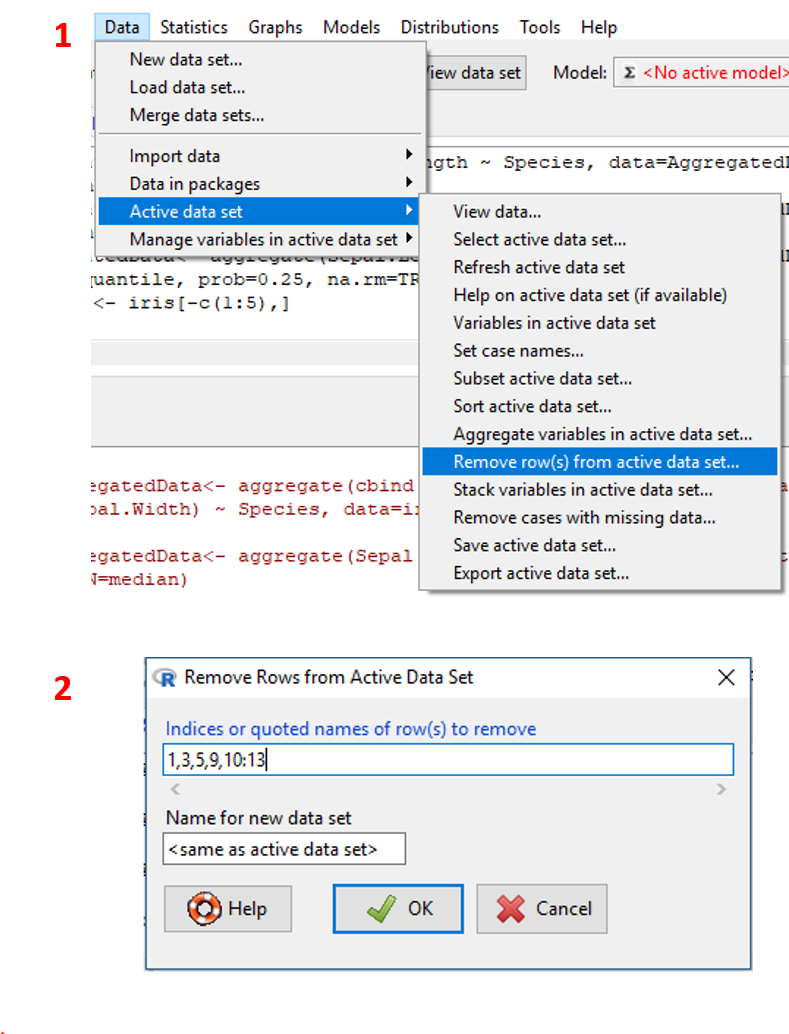
\includegraphics[width=0.7\linewidth]{./images/chp2/removerow} 

}

\caption{Tampilan tahapan melakukan drop observasi.}\label{fig:removerow}
\end{figure}

Sintaks yang digunakan untuk melakukan \emph{drop} baris observasi secara umu adalah sebagai berikut:

\begin{Shaded}
\begin{Highlighting}[]
\NormalTok{datasetbaru <-}\StringTok{ }\NormalTok{dataset[}\OperatorTok{-}\KeywordTok{c}\NormalTok{(indeks),]}
\end{Highlighting}
\end{Shaded}

\begin{longtable}[]{@{}llll@{}}
\caption{\label{tab:remove} Penjelasan item jendela remove rows from active data set.}\tabularnewline
\toprule
\begin{minipage}[b]{0.04\columnwidth}\raggedright
\textbf{No.}\strut
\end{minipage} & \begin{minipage}[b]{0.14\columnwidth}\raggedright
\textbf{Item}\strut
\end{minipage} & \begin{minipage}[b]{0.09\columnwidth}\raggedright
\textbf{Jenis Input}\strut
\end{minipage} & \begin{minipage}[b]{0.61\columnwidth}\raggedright
\textbf{Keterangan}\strut
\end{minipage}\tabularnewline
\midrule
\endfirsthead
\toprule
\begin{minipage}[b]{0.04\columnwidth}\raggedright
\textbf{No.}\strut
\end{minipage} & \begin{minipage}[b]{0.14\columnwidth}\raggedright
\textbf{Item}\strut
\end{minipage} & \begin{minipage}[b]{0.09\columnwidth}\raggedright
\textbf{Jenis Input}\strut
\end{minipage} & \begin{minipage}[b]{0.61\columnwidth}\raggedright
\textbf{Keterangan}\strut
\end{minipage}\tabularnewline
\midrule
\endhead
\begin{minipage}[t]{0.04\columnwidth}\raggedright
1.\strut
\end{minipage} & \begin{minipage}[t]{0.14\columnwidth}\raggedright
Indices or quoted\ldots{}\strut
\end{minipage} & \begin{minipage}[t]{0.09\columnwidth}\raggedright
\emph{text input}\strut
\end{minipage} & \begin{minipage}[t]{0.61\columnwidth}\raggedright
indeks atau nama baris yang akan di \emph{drop} atau di hapus\strut
\end{minipage}\tabularnewline
\begin{minipage}[t]{0.04\columnwidth}\raggedright
2.\strut
\end{minipage} & \begin{minipage}[t]{0.14\columnwidth}\raggedright
Name for new data set\strut
\end{minipage} & \begin{minipage}[t]{0.09\columnwidth}\raggedright
\emph{text input}\strut
\end{minipage} & \begin{minipage}[t]{0.61\columnwidth}\raggedright
input nama dataset baru yang dihasilkan\strut
\end{minipage}\tabularnewline
\bottomrule
\end{longtable}

\hypertarget{melakukan-drop-observasi-dengan-missing-value}{%
\subsection{\texorpdfstring{Melakukan \emph{Drop} Observasi dengan \emph{Missing Value}}{Melakukan Drop Observasi dengan Missing Value}}\label{melakukan-drop-observasi-dengan-missing-value}}

Selain menggunakan submenu \texttt{subset\ active\ data\ set}, \emph{drop missing value} dapat pula dilakukan dengan menggunakan submenu \texttt{remove\ cases\ with\ missing\ data}. Perbedaan antara metode pertama dan kedua adalah pada metode kedua \emph{drop missing value} dilakukan pada seluruh variabel dalam dataset. Tahapan untuk melakukannya adalah sebagai berikut:

\begin{enumerate}
\def\labelenumi{\arabic{enumi}.}
\tightlist
\item
  Pada menu \texttt{Data}, klik \texttt{Data/Active\ data\ set/Remove\ cases\ with\ missing\ data...}.
\item
  Spesifikan variabel yang akan dipilih untuk dataset baru dan nama output dataset (lihat Tabel \ref{tab:missing}). Klik \texttt{OK}.
\item
  Untuk mengecek dataset, klik \emph{toolbar} \texttt{View\ data\ set}.
\end{enumerate}

Visualisasi tahapan tersebut ditampilkan pada Gambar \ref{fig:missingval}.

\begin{figure}

{\centering 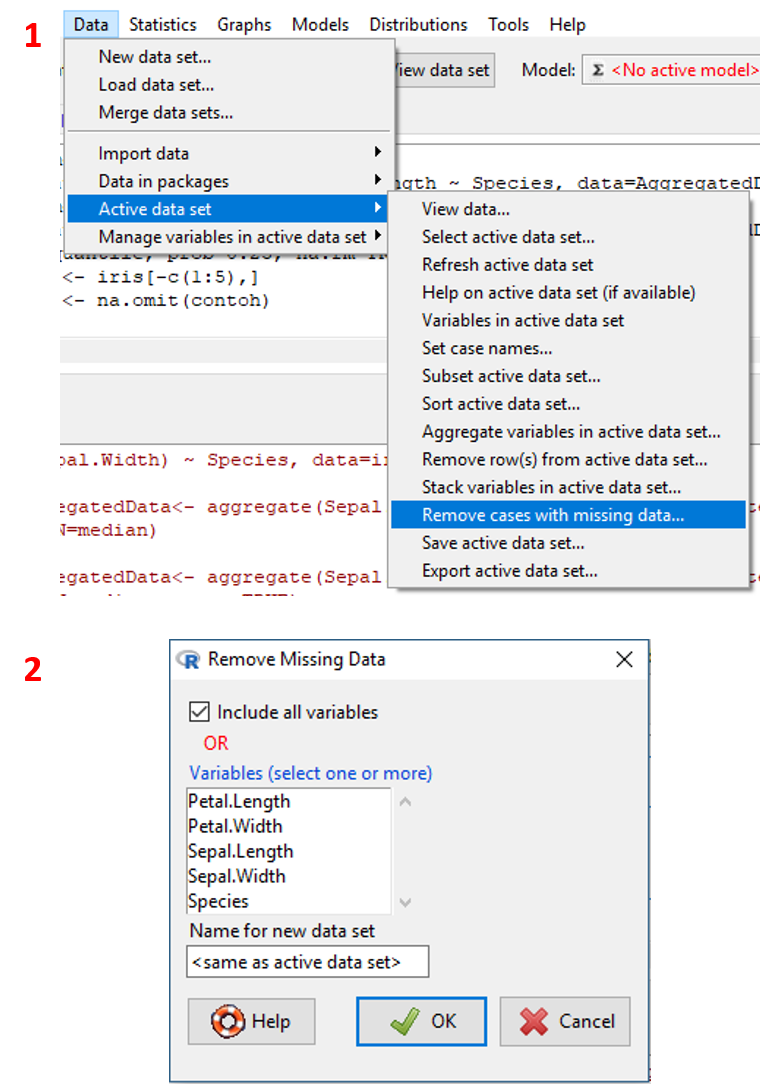
\includegraphics[width=0.7\linewidth]{./images/chp2/missingval} 

}

\caption{Tampilan tahapan melakukan drop observasi dengan missing value.}\label{fig:missingval}
\end{figure}

Sintaks untuk melakukan \emph{drop missing value} pada seluruh variabel dalam dataset secara umum adalah sebagai berikut:

\begin{Shaded}
\begin{Highlighting}[]
\NormalTok{datasetbaru <-}\StringTok{ }\KeywordTok{na.omit}\NormalTok{(dataset)}
\end{Highlighting}
\end{Shaded}

\begin{longtable}[]{@{}llll@{}}
\caption{\label{tab:missing} Penjelasan item jendela remove missing data.}\tabularnewline
\toprule
\begin{minipage}[b]{0.04\columnwidth}\raggedright
\textbf{No.}\strut
\end{minipage} & \begin{minipage}[b]{0.14\columnwidth}\raggedright
\textbf{Item}\strut
\end{minipage} & \begin{minipage}[b]{0.09\columnwidth}\raggedright
\textbf{Jenis Input}\strut
\end{minipage} & \begin{minipage}[b]{0.61\columnwidth}\raggedright
\textbf{Keterangan}\strut
\end{minipage}\tabularnewline
\midrule
\endfirsthead
\toprule
\begin{minipage}[b]{0.04\columnwidth}\raggedright
\textbf{No.}\strut
\end{minipage} & \begin{minipage}[b]{0.14\columnwidth}\raggedright
\textbf{Item}\strut
\end{minipage} & \begin{minipage}[b]{0.09\columnwidth}\raggedright
\textbf{Jenis Input}\strut
\end{minipage} & \begin{minipage}[b]{0.61\columnwidth}\raggedright
\textbf{Keterangan}\strut
\end{minipage}\tabularnewline
\midrule
\endhead
\begin{minipage}[t]{0.04\columnwidth}\raggedright
1.\strut
\end{minipage} & \begin{minipage}[t]{0.14\columnwidth}\raggedright
Include all variables\strut
\end{minipage} & \begin{minipage}[t]{0.09\columnwidth}\raggedright
\emph{check box}\strut
\end{minipage} & \begin{minipage}[t]{0.61\columnwidth}\raggedright
pilihan apakah akan menyertakan seluruh variabel pada dataset baru atau tidak\strut
\end{minipage}\tabularnewline
\begin{minipage}[t]{0.04\columnwidth}\raggedright
2.\strut
\end{minipage} & \begin{minipage}[t]{0.14\columnwidth}\raggedright
Variables\strut
\end{minipage} & \begin{minipage}[t]{0.09\columnwidth}\raggedright
\emph{select box}\strut
\end{minipage} & \begin{minipage}[t]{0.61\columnwidth}\raggedright
daftar variabel yang dapat dipilih untuk disertakan dalam dataset baru\strut
\end{minipage}\tabularnewline
\begin{minipage}[t]{0.04\columnwidth}\raggedright
3.\strut
\end{minipage} & \begin{minipage}[t]{0.14\columnwidth}\raggedright
Name for new data set\strut
\end{minipage} & \begin{minipage}[t]{0.09\columnwidth}\raggedright
\emph{text input}\strut
\end{minipage} & \begin{minipage}[t]{0.61\columnwidth}\raggedright
input nama dataset baru\strut
\end{minipage}\tabularnewline
\bottomrule
\end{longtable}

\hypertarget{mengelompokkan-variabel-menjadi-variabel-factor-dan-nilai}{%
\subsection{\texorpdfstring{Mengelompokkan Variabel Menjadi Variabel \emph{Factor} dan Nilai}{Mengelompokkan Variabel Menjadi Variabel Factor dan Nilai}}\label{mengelompokkan-variabel-menjadi-variabel-factor-dan-nilai}}

Submenu \texttt{stack\ variables\ in\ active\ data\ set} membuat sebuah dataset baru dimana dua atau lebih variabel ditumpuk menjadi variabel satu variabel dengan nilai variabel sebelumnya ditampilkan pada variabel nilai. Jika terdapat \(n\) observasi dalam dataset dan \(k\) variabel, maka dataset baru akan terdiri dari 2 variabel (\emph{factor} dan \emph{numeric}) dan \(n\times k\) observasi. Tahapan untuk melakukannya adalah sebagai berikut:

\begin{enumerate}
\def\labelenumi{\arabic{enumi}.}
\tightlist
\item
  Pada menu \texttt{Data}, klik \texttt{Data/Active\ data\ set/Stack\ variables\ in\ active\ data\ set...}.
\item
  Spesifikan variabel yang akan dipilih untuk dataset baru dan nama output dataset (lihat Tabel \ref{tab:stack}). Klik \texttt{OK}.
\item
  Untuk mengecek dataset, klik \emph{toolbar} \texttt{View\ data\ set}.
\end{enumerate}

Visualisasi tahapan tersebut ditampilkan pada Gambar \ref{fig:stackvar}.

\begin{figure}

{\centering 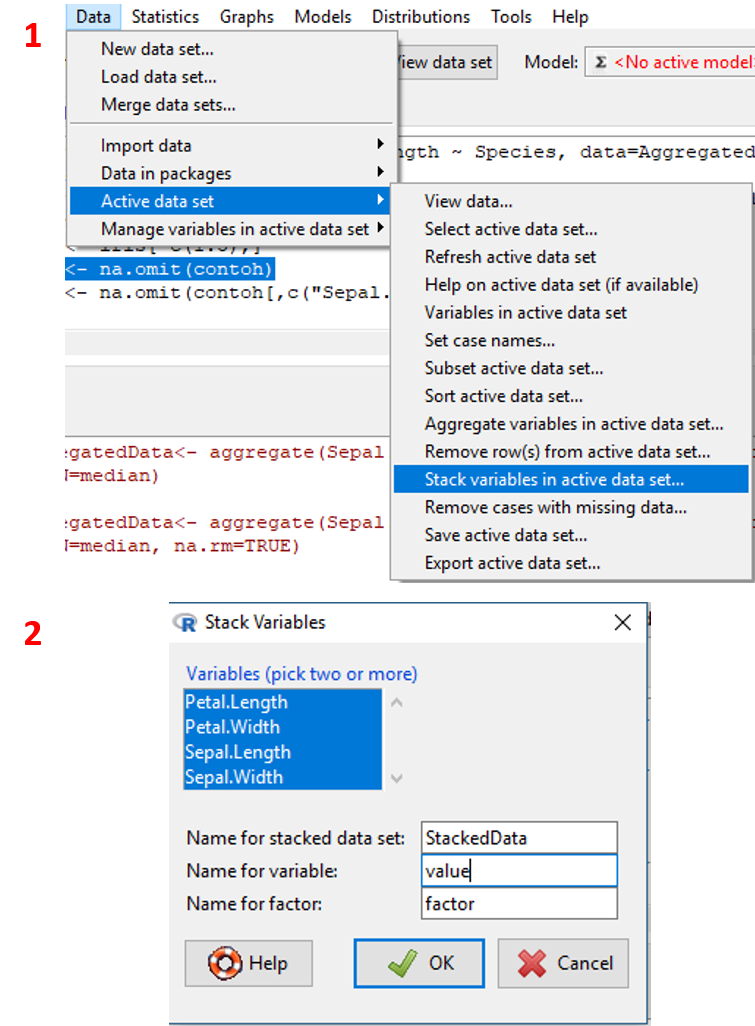
\includegraphics[width=0.7\linewidth]{./images/chp2/stackvar} 

}

\caption{Tampilan tahapan mengelompokkan variabel menjadi variabel factor dan nilai.}\label{fig:stackvar}
\end{figure}

Terdapat dua buah sintaks dalam melakukan proses pengelompokan data. Sintaks pertama melakukan pengelompokan data, sedangkan sintaks kedua merubah nama kolom dataset baru. Kedua sintaks tersebut adalah sebagai berikut:

\begin{Shaded}
\begin{Highlighting}[]
\NormalTok{datasetbaru <-}\StringTok{ }\KeywordTok{stack}\NormalTok{(dataset[, }\KeywordTok{c}\NormalTok{(}\StringTok{"variabel1"}\NormalTok{,}\StringTok{"variabel2"}\NormalTok{,..)])}
\KeywordTok{names}\NormalTok{(datasetbaru) <-}\StringTok{ }\KeywordTok{c}\NormalTok{(}\StringTok{"value"}\NormalTok{, }\StringTok{"factor"}\NormalTok{)}
\end{Highlighting}
\end{Shaded}

\begin{longtable}[]{@{}llll@{}}
\caption{\label{tab:stack} Penjelasan item jendela stack variables.}\tabularnewline
\toprule
\begin{minipage}[b]{0.04\columnwidth}\raggedright
\textbf{No.}\strut
\end{minipage} & \begin{minipage}[b]{0.14\columnwidth}\raggedright
\textbf{Item}\strut
\end{minipage} & \begin{minipage}[b]{0.09\columnwidth}\raggedright
\textbf{Jenis Input}\strut
\end{minipage} & \begin{minipage}[b]{0.61\columnwidth}\raggedright
\textbf{Keterangan}\strut
\end{minipage}\tabularnewline
\midrule
\endfirsthead
\toprule
\begin{minipage}[b]{0.04\columnwidth}\raggedright
\textbf{No.}\strut
\end{minipage} & \begin{minipage}[b]{0.14\columnwidth}\raggedright
\textbf{Item}\strut
\end{minipage} & \begin{minipage}[b]{0.09\columnwidth}\raggedright
\textbf{Jenis Input}\strut
\end{minipage} & \begin{minipage}[b]{0.61\columnwidth}\raggedright
\textbf{Keterangan}\strut
\end{minipage}\tabularnewline
\midrule
\endhead
\begin{minipage}[t]{0.04\columnwidth}\raggedright
1.\strut
\end{minipage} & \begin{minipage}[t]{0.14\columnwidth}\raggedright
Variables\strut
\end{minipage} & \begin{minipage}[t]{0.09\columnwidth}\raggedright
\emph{select box}\strut
\end{minipage} & \begin{minipage}[t]{0.61\columnwidth}\raggedright
daftar variabel yang dapat dipilih untuk dikelompokkan\strut
\end{minipage}\tabularnewline
\begin{minipage}[t]{0.04\columnwidth}\raggedright
2.\strut
\end{minipage} & \begin{minipage}[t]{0.14\columnwidth}\raggedright
Name for staked data..\strut
\end{minipage} & \begin{minipage}[t]{0.09\columnwidth}\raggedright
\emph{text input}\strut
\end{minipage} & \begin{minipage}[t]{0.61\columnwidth}\raggedright
nama dataset baru hasil pengelompokan\strut
\end{minipage}\tabularnewline
\begin{minipage}[t]{0.04\columnwidth}\raggedright
3.\strut
\end{minipage} & \begin{minipage}[t]{0.14\columnwidth}\raggedright
Name for variable\strut
\end{minipage} & \begin{minipage}[t]{0.09\columnwidth}\raggedright
\emph{text input}\strut
\end{minipage} & \begin{minipage}[t]{0.61\columnwidth}\raggedright
nama variabel nilai hasil pengelompokkan\strut
\end{minipage}\tabularnewline
\begin{minipage}[t]{0.04\columnwidth}\raggedright
4.\strut
\end{minipage} & \begin{minipage}[t]{0.14\columnwidth}\raggedright
Name for factor\strut
\end{minipage} & \begin{minipage}[t]{0.09\columnwidth}\raggedright
\emph{text input}\strut
\end{minipage} & \begin{minipage}[t]{0.61\columnwidth}\raggedright
nama variabel \emph{factor} hasil pengelompokan nama variabel pada dataset sebelumnya\strut
\end{minipage}\tabularnewline
\bottomrule
\end{longtable}

\hypertarget{menggabungkan-dua-dataset}{%
\subsection{Menggabungkan Dua Dataset}\label{menggabungkan-dua-dataset}}

Untuk menggabungkan dua buah dataset, kedua dataset perlu memiliki elemen kunci yang sama. Secara \emph{default} \texttt{R\ Commander} mengambil \emph{rownames} sebagai elemen kunci, sehingga elemen kunci yang dimiliki oleh masing-masing dataframe haruslah konsisten satu sama lain. Penggabungan dataset dapat dilakukan melalui penggabungan kolom dan baris. Penggabungan juga dapat dilakukan melalui elemen unik dari baris maupun kolom. Maksudnya adalah \texttt{R\ Commander} hanya menggabungkan dataset yang memiliki elemen kunci sama (\emph{rownames} sama) pada kedua dataset. Jika terdapat observasi pada dataset 1 dan tidak memiliki \emph{rownames} atau elemen kunci sama pada dataset 2, maka observasi tersebut akan dihapus dari proses penggabungan data. Tahapan penggabungan dua buah dataset adalah sebagai berikut:

\begin{enumerate}
\def\labelenumi{\arabic{enumi}.}
\tightlist
\item
  Pada menu \texttt{Data}, klik \texttt{Data/Merge\ data\ set...}.
\item
  Pada jendela yang muncul, klik dataset yang akan digabungkan dan cara penggabungannya (lihat Tabel \ref{tab:merge}). Klik \texttt{OK}.
\item
  Untuk mengecek dataset, klik \emph{toolbar} \texttt{View\ data\ set}.
\end{enumerate}

Visualisasi tahapan tersebut ditampilkan pada Gambar \ref{fig:mergedata}.

\begin{figure}

{\centering 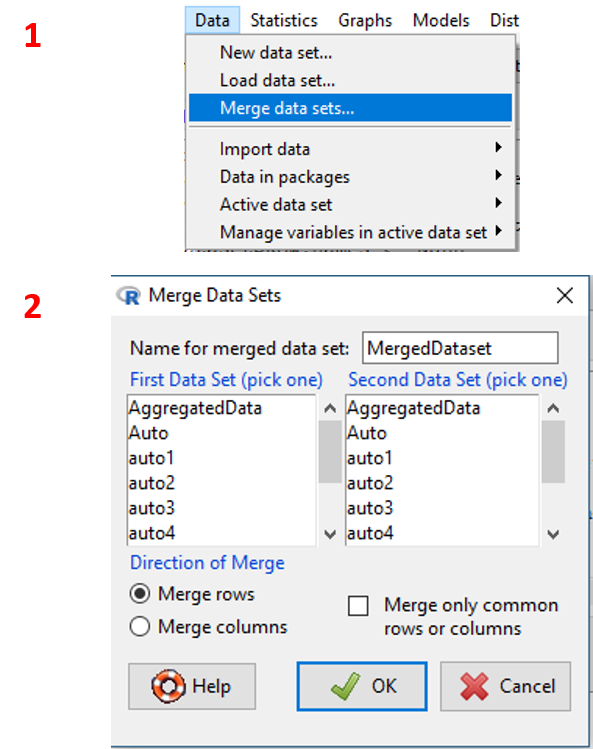
\includegraphics[width=0.7\linewidth]{./images/chp2/merge} 

}

\caption{Tampilan tahapan menggabungkan dua buah dataset.}\label{fig:mergedata}
\end{figure}

Sintaks yang digunakan untuk menggabungkan dua buah dataset secara umum adalah sebagai berikut:

\begin{Shaded}
\begin{Highlighting}[]
\CommentTok{# penggabungan baris tanpa mempertimbangkan}
\CommentTok{# elemen unik}
\NormalTok{datasetbaru <-}\StringTok{ }\KeywordTok{mergeRows}\NormalTok{(data1, data2, }\DataTypeTok{common.only=}\OtherTok{FALSE}\NormalTok{)}

\CommentTok{# pengagbungan kolom dengan mempertimbangkan}
\CommentTok{# elemen unik}
\NormalTok{datasetbaru <-}\StringTok{ }\KeywordTok{merge}\NormalTok{(data1, data2, }\DataTypeTok{all=}\OtherTok{FALSE}\NormalTok{, }\DataTypeTok{by=}\StringTok{"row.names"}\NormalTok{)}
\KeywordTok{rownames}\NormalTok{(datasetbaru) <-}\StringTok{ }\NormalTok{datasetbaru}\OperatorTok{$}\NormalTok{Row.names}
\NormalTok{datasetbaru}\OperatorTok{$}\NormalTok{Row.names <-}\StringTok{ }\OtherTok{NULL}
\end{Highlighting}
\end{Shaded}

\begin{longtable}[]{@{}llll@{}}
\caption{\label{tab:merge} Penjelasan item jendela merge data sets.}\tabularnewline
\toprule
\begin{minipage}[b]{0.04\columnwidth}\raggedright
\textbf{No.}\strut
\end{minipage} & \begin{minipage}[b]{0.14\columnwidth}\raggedright
\textbf{Item}\strut
\end{minipage} & \begin{minipage}[b]{0.09\columnwidth}\raggedright
\textbf{Jenis Input}\strut
\end{minipage} & \begin{minipage}[b]{0.61\columnwidth}\raggedright
\textbf{Keterangan}\strut
\end{minipage}\tabularnewline
\midrule
\endfirsthead
\toprule
\begin{minipage}[b]{0.04\columnwidth}\raggedright
\textbf{No.}\strut
\end{minipage} & \begin{minipage}[b]{0.14\columnwidth}\raggedright
\textbf{Item}\strut
\end{minipage} & \begin{minipage}[b]{0.09\columnwidth}\raggedright
\textbf{Jenis Input}\strut
\end{minipage} & \begin{minipage}[b]{0.61\columnwidth}\raggedright
\textbf{Keterangan}\strut
\end{minipage}\tabularnewline
\midrule
\endhead
\begin{minipage}[t]{0.04\columnwidth}\raggedright
1.\strut
\end{minipage} & \begin{minipage}[t]{0.14\columnwidth}\raggedright
Name for merge data set\strut
\end{minipage} & \begin{minipage}[t]{0.09\columnwidth}\raggedright
\emph{text input}\strut
\end{minipage} & \begin{minipage}[t]{0.61\columnwidth}\raggedright
input nama dataset baru\strut
\end{minipage}\tabularnewline
\begin{minipage}[t]{0.04\columnwidth}\raggedright
2.\strut
\end{minipage} & \begin{minipage}[t]{0.14\columnwidth}\raggedright
First Data set\strut
\end{minipage} & \begin{minipage}[t]{0.09\columnwidth}\raggedright
\emph{select box}\strut
\end{minipage} & \begin{minipage}[t]{0.61\columnwidth}\raggedright
daftar dataset pertama yang akan digabung\strut
\end{minipage}\tabularnewline
\begin{minipage}[t]{0.04\columnwidth}\raggedright
3.\strut
\end{minipage} & \begin{minipage}[t]{0.14\columnwidth}\raggedright
Second Data set\strut
\end{minipage} & \begin{minipage}[t]{0.09\columnwidth}\raggedright
\emph{select box}\strut
\end{minipage} & \begin{minipage}[t]{0.61\columnwidth}\raggedright
daftar dataset kedua yang akan digabung\strut
\end{minipage}\tabularnewline
\begin{minipage}[t]{0.04\columnwidth}\raggedright
4.\strut
\end{minipage} & \begin{minipage}[t]{0.14\columnwidth}\raggedright
Direction or Merge\strut
\end{minipage} & \begin{minipage}[t]{0.09\columnwidth}\raggedright
\emph{radio button}\strut
\end{minipage} & \begin{minipage}[t]{0.61\columnwidth}\raggedright
pilihan cara penggabungan\strut
\end{minipage}\tabularnewline
\begin{minipage}[t]{0.04\columnwidth}\raggedright
5.\strut
\end{minipage} & \begin{minipage}[t]{0.14\columnwidth}\raggedright
Merge only common\ldots{}\strut
\end{minipage} & \begin{minipage}[t]{0.09\columnwidth}\raggedright
\emph{check box}\strut
\end{minipage} & \begin{minipage}[t]{0.61\columnwidth}\raggedright
opsi apakah hanya observasi dengan elemen unik yang ada pada dua buah dataset yang akan digabungkan\strut
\end{minipage}\tabularnewline
\bottomrule
\end{longtable}

\hypertarget{modifikasi-lainnya}{%
\subsection{Modifikasi Lainnya}\label{modifikasi-lainnya}}

\hypertarget{ringkasan-dan-visualisasi-data}{%
\chapter{Ringkasan dan Visualisasi Data}\label{ringkasan-dan-visualisasi-data}}

\hypertarget{uji-statistik-sederhana}{%
\chapter{Uji Statistik Sederhana}\label{uji-statistik-sederhana}}

\hypertarget{linier-dan-generalized-linear-model}{%
\chapter{\texorpdfstring{Linier dan \emph{Generalized Linear} Model}{Linier dan Generalized Linear Model}}\label{linier-dan-generalized-linear-model}}

\hypertarget{distribusi-probabilitas-dan-simulasi}{%
\chapter{Distribusi Probabilitas dan Simulasi}\label{distribusi-probabilitas-dan-simulasi}}

\hypertarget{referensi}{%
\chapter*{Referensi}\label{referensi}}


\begin{enumerate}
\def\labelenumi{\arabic{enumi}.}
\tightlist
\item
  Fox, J. 2005. \textbf{The R Commander: A Basic-Statistics Graphical User Interface to R}. Journal of Statistical Software.Vol:14(9), p:1-42.
\item
  Fox, J. 2017. \textbf{Using the R Commader: A Point-and-Click Interface for R}. CRC Press.
\item
  Fox, J. Valat, M.B. 2018. \textbf{Getting Started With the R Commander}.\url{https://socialsciences.mcmaster.ca/jfox/Misc/Rcmdr/Getting-Started-with-the-Rcmdr.pdf}.
\item
  Gio, P.U. Irawan, D.E. 2016. \textbf{Belajar Statistika dengan R (disertai beberapa contoh perhitungan manual)}. USU Press : Medan.
\item
  Nguyen-Feng, V. Stellmack, M.A.~2016. \textbf{A Guide to Data Aalysis in R Commander}. University of Minnesota.
\item
  Primartha, R. 2018. \textbf{Belajar Machine Learning Teori dan Praktik}. Penerbit Informatika : Bandung.
\item
  Quick-R. \textbf{Data Input}. \url{https://www.statmethods.net/input/index.html}
\item
  Quick-R. \textbf{Data Management}. \url{https://www.statmethods.net/management/index.html}
\item
  Rosadi,D. 2011. \textbf{Analisis Ekonometrika dan Runtun Waktu Terapan dengan R}. Penerbit Andi: Yogyakarta.
\item
  Rosadi,D. 2016. \textbf{Analisis Statistika dengan R}. Gadjah Mada University Press: Yogyakarta.
\item
  Rosidi, M. 2019. \textbf{Metode Numerik Menggunakan R Untuk Teknik Lingkungan}. \url{https://bookdown.org/moh_rosidi2610/Metode_Numerik/}.
\item
  STHDA. \textbf{Importing Data Into R }. \url{http://www.sthda.com/english/wiki/importing-data-into-r}
\item
  STHDA. \textbf{Exporting Data From R}. \url{http://www.sthda.com/english/wiki/exporting-data-from-r}
\item
  STDHA. \textbf{Getting Help With Functions In R Programming}. \url{http://www.sthda.com/english/wiki/getting-help-with-functions-in-r-programming} .
\item
  Venables, W.N. Smith D.M. and R Core Team. 2018. \textbf{An Introduction to R}. R Manuals.
\item
  Wickham, H. Grolemund G. 2016. \textbf{R For Data Science: Import, Tidy, Transform, Visualize, And Model Data}. O'Reilly Media, Inc.
\item
  Widodo, B. Rachmawati, R.N. 2013. \textbf{Pengantar Praktis Pemrograman R untuk Ilmu Komputer}. Halaman Moeka Publishing : Jakarta.
\end{enumerate}

\bibliography{book.bib,packages.bib}

\backmatter
\printindex


\end{document}
